
\documentclass[11pt,a4paper]{article}

\usepackage[english]{babel}
\usepackage[T1]{fontenc}
\usepackage{lmodern}
\usepackage[a4paper,margin=1in]{geometry}

\usepackage{xcolor}
\usepackage{graphicx}
\usepackage{float}
\usepackage{booktabs}
\usepackage{array}
\usepackage{caption}
\usepackage{subcaption}
\usepackage{tabularx}

\usepackage{amsmath,amssymb,bm}
\usepackage{enumitem}
\usepackage{titlesec}
\usepackage[authoryear]{natbib}
\usepackage{hyperref}
\usepackage{fancyhdr}
\usepackage{pdflscape}
\usepackage{xfrac}
\usepackage{booktabs}
\usepackage{threeparttable}
\usepackage{multirow}
\usepackage{adjustbox}
\usepackage{rotating}


\usepackage{tikz}
\usetikzlibrary{arrows.meta, positioning, shapes.geometric}

\definecolor{darkblue}{rgb}{0,0,0.8}
\hypersetup{
	colorlinks=true,
	citecolor=darkblue,
	linkcolor=darkblue,
	urlcolor=darkblue
}

\setlength{\parskip}{0.55em}
\setlength{\parindent}{0pt}
\begin{document}
	

\tableofcontents

\pagebreak

% =============================================================================
%                         SECTION 1: INTRODUCTION
% =============================================================================

%<*ch1body>
\section{Introduction}
\label{ch1:sec:introduction}

Capacity utilization occupies a contested position in political economy because
it mediates between the two questions that define accumulation theory: how much
productive capacity does an economy possess, and what fraction of it is being
used? The answer to the first determines the structural trajectory of capital
accumulation; the answer to the second determines whether demand shortfalls
carry durable consequences for investment, employment, and distribution. The
Neo-Kaleckian tradition argues that the normal rate of utilization is endogenous
to demand history, making path-dependence a structural feature of accumulation
\citep{Lavoie1995,Nikiforos2013,Setterfield2020}. The Sraffian-Keynesian
tradition argues that utilization gravitates toward a structurally given normal
rate determined by cost conditions and competitive pressures, so that
demand-side interventions have only transitory effects on accumulation
\citep{Ciccone1986,GirardiPariboni2016,GahnGonzalez2022}. The stakes are not
merely theoretical: if utilization is path-dependent, macroeconomic governance
can reshape accumulation trajectories; if it converges, the space for such
intervention is structurally bounded.

This chapter makes three contributions. First, to the heterodox measurement
debate: the instruments available to both sides of the Kaleckian--Sraffian
controversy cannot settle the question they are deployed to adjudicate---the
Federal Reserve Board's capacity utilization series was built to produce a
stable, institutionally credible signal for monetary policy governance within a
historically specific Fordist settlement \citep{Shapiro1989,Board2017}, and its
stationarity is a design feature, not a discovered property of the data; both
sides of the controversy have recruited the same governance instrument into a
scientific context without examining the transit
\citep{Nikiforos2016,Nikiforos2021}. Second, to the methodology of critical
replication in political economy: adapting the \citet{HerndonAshPollin2014}
audit framework to a cointegration setting exposes the same researcher degrees
of freedom---specification selection, weighting, sample
composition---operating in the measurement of productive capacity as in Reinhart
and Rogoff's growth-debt threshold. Third, to system cointegration in heterodox
economics: Johansen methods have not been applied to the capacity utilization
question, leaving the single-equation ARDL as the unchallenged estimator for a
structural object that requires system identification.

\citet{Shaikh2016} provides the only intervention in the political economy
literature that proceeds independently of this controversy. His identification
strategy recovers productive capacity as the long-run component of the
output--capital cointegrating relation under a maintained normal-utilization
closure, and the empirical finding this strategy produces is unbalanced growth:
the elasticity of productive capacities with respect to accumulation
demand---the transformation elasticity $\theta$---is persistently below unity,
breaking the balanced-growth assumption shared by both the Kaleckian and
Sraffian positions. The limit of the approach is architectural. The
single-equation ARDL specification captures unbalanced growth through a fixed
elasticity when the theory predicts that $\theta$ is distributionally
conditioned---regime-specific rather than structurally constant. The
discretionary dummy structures required to sustain the long-run relationship
signal precisely that distribution matters, without providing a variable through
which it can act.

The critical replication developed here subjects this identification to
progressive scrutiny across four stages, each releasing one constraint that
Shaikh's estimation held fixed. Stage~S0 reconstructs the benchmark
specification and asks whether the published result can be reproduced under
current-release data. Stage~S1 releases the lag-order constraint and maps the
full admissible ARDL specification grid, asking whether the capacity anchor is a
property of the specification family or an artifact of a particular lag
selection. Stage~S2 releases the single-equation conditioning structure and
re-estimates the long-run restriction as a system property via Johansen VECM,
asking whether the co-integrating vector survives escalation from conditional to
joint identification. Stage~S3 releases the temporal pooling assumption and
tests whether the scalar $\theta$ masks regime variation across the
Fordist/Post-Fordist threshold. Before the replication, a historical trace
reconstructs how capacity utilization became a governance variable under Fordist
and post-Fordist accumulation regimes
(Section~\ref{sec:historical_trace}), and a conceptual framework derives the
elasticity of productive capacities with respect to accumulation demand from
accounting identities and closure rules, establishing the theoretical object the
replication must recover and the conditions under which its regime-dependence
becomes identifiable (Section~\ref{sec:conceptual_framework}). The four-stage
replication and its results are presented in
Section~\ref{sec:critical_replication}; Section~\ref{sec:conclusion} concludes.

\section{Historical Trace of Capacity Utilization Measurement throughout Fordist to Post-Fordist era} 
\label{sec:historical_trace}

Capacity utilization measurement is not a narrow sequence of statistical
refinements but a history of statecraft: capitalist development adopting
operational routines of macroeconomic measurement within and across different
institutional configurations. Under a regulationist approach, operational
routines are not neutral tools. They are institutionalized forms of ideological
embeddedness shaping state capacities to implement macroeconomic policy as
\textit{spatio-temporal fixes} \citep{Jessop2003,Jessop2006}: strategic
selectivities on what counts as the relevant macroeconomic signal, which
institutions are authorized to act on it, and over what temporal horizon they are
expected to intervene. For that same reason, however, they can also become sources
of dysfunction when the contradictions they once regularized overcome the state
capacities to offset them. What matters is not measurement practices themselves,
but the political economy through which they are constructed, interpreted,
stabilized, repurposed, and contested across changing accumulation regimes.

The earliest large-scale attempt to measure the slack of productive capacities in
the United States emerged not from a mature macroeconomic policy apparatus but
from the Brookings Institution, in the aftermath of the Great Depression.
Brookings' economists expanded empirical economic inquiry into the production,
consumption, capital formation, and income of the United States, presenting the
first efforts to estimate the nation's productive ceiling sector by sector
\citep{Nourse1934}. That shift made visible what counted as idle capacities in the
first place, pioneering the operational routines that would later constitute a
policy dashboard. Capacity utilization was assembled historically through
institutional inquiry, statistical construction, and policy need---from the
outset, the measurement issue was inseparable from the problem of statecraft.

\subsection{From Survey Measures to an Inflation Sentinel: Capacity Utilization Measurements during the Fordist Era}
\label{subsec:21_fordist_capacity_utilization}

The Fordist history of capacity utilization measurement begins with a problem of governability rather than with a settled variable. In the United States, the Great Depression made idle resources visible as a political and administrative problem, but not yet as a stabilized object of macroeconomic management. What had to be built first was a way of rendering productive slack as statistically legible. Brookings' research was decisive because it turned unused productive capacity from an impressionistic sign of downturn into a measurable ceiling. The stakes were no longer whether factories stood idle, but how far actual output fell short of a plausible productive limit and under what conventions that limit should be defined. Capacity utilization thus entered macroeconomic discourse as an operational problem of visibility: institutions had to decide what counted as ``capacity,'' how it could be approximated, and how that approximation could steer interventions of macroeconomic policy. Later assessments made clear that this early construction of the object rested on unresolved tensions between notions of engineering and economic capacities \citep{Burns1954,KleinDavid1958}. The early history of utilization measurement was therefore already a history of governance by numbers rather than a neutral exercise in statistical description.

American Keynesianism gave that problem a clearer institutional and theoretical function. Alvin Hansen’s interwar and wartime seminal thesis on secular stagnation helped explain why slack could no longer remain a residual category once stabilization became a policy objective \citep{Hansen1936,Hansen1941, Barber1987}. Hicks and Samuelson then carried that problem into a more formal and pedagogical macroeconomic grammar, helping turn slack into a governable macroeconomic object rather than a residual business-cycle symptom, by means of developing the educational toolkit that would shape the training of economists at higher education institutions, shaping the economic discipline in the United States under the IS-LM framework \citep{Hicks1937,Samuelson1947,Samuelson1948}. Once the state was expected to manage demand, sustain employment, and monitor bottlenecks, it needed indicators that translated underutilized productive resources into signals for fiscal and/or monetary policy intervention. Capacity utilization became necessary not because Keynesianism discovered a timeless economic magnitude, but because a policy regime guided by the notion of full-employment required an index through which effective-demand deficiencies could be rendered legible to authorities charged with stabilization. That shift mattered because it moved utilization measurement from descriptive inquiry into the core of a policy dashboard. The state did not govern an abstract ``economy'' in general. It governed through a portfolio of indicators that identified idle resources, pressures, and thresholds for intervention. In that setting, utilization was never merely technical. It was bound to a historically specific settlement in which demand management, employment commitments, and macroeconomic expertise reinforced one another.

That theoretical consolidation did not by itself settle the routine. McGraw--Hill Publishing Company did much of that work. Its plant-and-equipment surveys regularized managerial reports of actual and ``preferred'' operating rates and, in doing so, converted heterogeneous and scattered notions of productive capacity into a repeated business-information device \citep{Butler1958,Phillips1963}. What mattered was less about overcoming ambiguous conceptualizations than about the creation of an administratively reproducible benchmark. Under Fordism, reproducibility itself became a source of authority. Repeated survey collection generated comparability across time and sectors, while the broader information infrastructure of \emph{monopoly capital} enhanced the legitimacy of its measurement inside business forecasting and policy discussion \citep{BaranSweezy1988,Munroe2007}. What emerged, then, was not simply a better estimate of productive ceilings, but a routinized operational device through which firms, analysts, and policymakers could speak a common language about slack. At the same time, the benchmark’s apparent neutrality rested on a dense set of conventions: assumptions about maintenance, overtime, sustainable operation, and the reporting practices of firms. Survey settlement therefore did not abolish mediation. It normalized it.


The Federal Reserve then transformed that settled routine into official macroeconomic authority \citep{Board2017}. Once capacity and utilization measures were incorporated into the Industrial Production program and disseminated the survey benchmark ceased to be merely one possible way of gauging slack, it became the official operational routine through which the state rendered idle productive capacities as a visible. That move altered the structure of the field. Institutional embedding did not simply add prestige to an existing measure; it raised the switching costs of alternatives and standardized what counted as admissible evidence. Physical-intensity measures such as Electric Motors Utilization and the Average Workweek of Capital remained conceptually important and in some respects tracked operational realities more directly, but they failed to secure comparable institutional adoption \citep{Foss1963,TaubmanGottschalk1971}. The point is not that every rival was empirically defeated. It is that one routine proved easier to reproduce administratively, became embedded in everyday bureaucratic practices, and got integrated into policy practice inside the state’s statistical machinery. In this way, capacity utilization became an official governance variable of Fordist macroeconomic demand management, a feature of the Keynesian National Welfare State \citep{Jessop2002}.

The crisis of the 1970s did not abolish that routine. It triggered the process of its recodification. Under stagflationary pressures, capacity utilization was increasingly detached from its earlier role as a signal of effective-demand slack and reinterpreted as a warning device for inflationary strain. The benchmark survived, but the admissible meaning of the benchmark narrowed. What had once helped justify expansionary intervention now mattered insofar as it signaled when effective output was triggering inflationary pressures. This shift appears clearly in the debates taking place at the Brookings Institution, where capacity measures were increasingly judged by whether they could register credible accounts of inflation \citep{KleinEtAl1973}. This was not a minor technical refinement. It marked a crisis-driven transformation in the policy dashboard itself. As the Bretton Woods order unraveled, the Fordist compromise weakened, and profitability pressures intensified, the utilization index was repurposed within a broader reorientation of macroeconomic governance. The same operational routine that had once helped organize full-employment management was now made compatible with emerging anti-inflation discipline. In regulationist terms, the benchmark persisted across a transition between modes of regulation \citep{Aglietta2000,Jessop2002}, but its place in the hierarchy of policy priorities changed decisively. That is why the recoding of capacity utilization should be read as a critical juncture in the fall of American Keynesianism rather than as a simple update in measurement techniques.

What survived this transition was not Keynesian slack governance itself, but the institutional durability of the routine. Survey-based utilization retained authority because it had already been stabilized inside the policy apparatus, and that durability made re-purposing easier than replacement. The Fordist history of capacity utilization measurement is therefore not one of rise and disappearance, but of construction, routinization, recoding, and transition. Brookings made slack visible as a measurable problem. American Keynesianism turned that problem into a functional requirement of stabilization. McGraw--Hill transformed the measure into a durable operational routine, and the Federal Reserve institutionalized it. The stagflation crisis then narrowed its meaning into an inflation sentinel. That sequence matters for what follows. Once the Fordist benchmark had been recoded in this way, the ground was prepared for a new measurement regime in which slack would increasingly be governed not through survey-centered utilization series, but through more portable output-gap and potential-output benchmarks aligned with post-Fordist forms of profit-oriented market discipline \citep{Jessop2002}.


% =============================================================================
% §2.2 — The Rise of Econometrics and its Global Sedimentation on Institutions
% CLEAN ASSEMBLED DRAFT — 2026-03-25
% =============================================================================
% COMPILE NOTES:
%   - natbib (author-year)
%   - Check bib keys: Foster2022 vs Foster2024 (verify in .bib)
%   - .bib additions needed: GrigoliEtAl2015, AastveitTrovik2014, BarbarinoBergeEtAl2020
%   - .bib deduplication pending: Jessop2002, Best2025, Sklair2000
% =============================================================================

\subsection{The Rise of Econometrics and its Global Sedimentation on Institutions: From Capacity Utilization to Output-Gap Measurement through Post-Fordist Times}
\label{subsec:22_postfordist_capacity_utilization}


% ---- R1 — Opening ----

Post-Fordism names not a periodization label but a reorganization of statecraft under conditions of spatio-temporal compression: the acceleration of capital circulation, the re-scaling of state authority toward supranational institutions, and the displacement of nationally bounded operational routines of demand management grounded in Keynesian doctrine by portable methods legible within the jargon of neoclassical economics. These methods operationalized inflation monitoring and macroeconomic surveillance across supranational institutions, equipping a modern technocratic bureaucracy with portable operational routines that could travel across national boundaries and scales of governance. In other words, the demise of Bretton Woods financial architecture cannot be reduced merely to free capital mobility that made possible demand management at national scale; rather, it was a process which also carried the flux of portable methodologies akin to the interests of finance: the hegemonic fraction of an emergent transnational capitalist class, whose discourse of globalization was carried by its bureaucratic and technical fractions \citep{Jessop2002,Jessop2003,Sklair2000}.

The spatio-temporal compression of globalization---faster shipping times, the increasing tendency to organize production systems around global value chains setting up a new international division of labour \citep{Frobel1978}, the accelerated development of data processing and telecommunications that built a common infrastructure for financial transactions (the Society for Worldwide Interbank Financial Telecommunication, established in 1973, is the clearest institutional marker)---created a historically specific governance demand. Inherited Fordist routines---national surveys, dashboard indicators, discretionary fiscal instruments---could no longer travel across the jurisdictions and institutional scales that globalized accumulation required \citep{Jessop2003}. What emerged in response was a tendency within post-Fordist macro governance: the withdrawal of the state from real-time discretionary demand management, and its replacement by rule-based, pre-announced policy frameworks whose authority rested not on the correct tracking of business cycles but on the institutional consensus that depoliticized technocratic routines could substitute for discretionary judgment \citep{SaadFilho2018}.

This tendency also rebranded the benchmark itself: in place of capacity utilization as a slack measure, the \emph{output gap} became the central concept for distinguishing cyclical from trend behavior in mainstream macroeconomics. Output-gap estimation was recast as a portable, institutionally reproducible governance variable ---reducing the complexity of identifying capacity utilization into a single benchmark legible to surveillance bodies, budget offices, and central banks simultaneously. Yet the shift to econometric measurement did not resolve the contradictions of governance under globalized accumulation. It displaced them---across geographies and temporal horizons \citep{Jessop2003}---until the Global Financial Crisis of 2008 placed the output-gap apparatus under pressures it was not designed to absorb.


% ---- R2 — Volcker Shock as Pivot ----

The decisive critical juncture through which this tendency consolidates is the Volcker Shock, which was not simply a victory of anti-inflation orthodoxy over Keynesian demand management. The institutional groundwork preceded the shock by at least two decades. From the 1960s onward, the re-emergence of international capital markets---Eurodollar lending, offshore credit intermediation, the progressive erosion of Bretton Woods capital controls---had already been reworking the structural foundations of U.S.\ financial power \citep{Konings2007}. The monetarist turn of the late 1970s should therefore be read not as a retreat of the state under external market pressure but as a reconfiguration of the balance of forces led by financial capital to reshape the international monetary order in its own image. \citet{Krippner2005} identifies the structural backdrop: by the time Volcker raised rates, profit accumulation had already been shifting from commodity production toward financial channels. The shock did not initiate that shift, but it consolidated the institutional conditions under which financial accumulation could become hegemonic.

What elite narratives would later present as technical correction---the triumph of sound money over inflationary irresponsibility---was in practice a political settlement with distributional consequences \citep{MorganSheehan2015}. The credibility that the Volcker intervention established was not self-sustaining. It had to be reproduced through new governance technologies. \citet{Krippner2007} traces how central bank transparency---the public communication of targets, forecasts, and decision rationales---was constructed during this period not as a neutral modernization of monetary practice but as a mechanism for managing expectations instead of demand. Transparency replaced discretion as the operating principle, and in doing so helped institutionalize the shift from a governance regime that acted on the economy to one that governed through the credibility of its own announced commitments.

The theoretical legitimation for that regime shift had been assembled in the preceding decade. \citet{Johnson2024} reconstructs the Lucas critique not as a laissez-faire manifesto but as an argument about what kind of governance could count as scientific. Lucas did not reject state intervention as such. He rejected discretionary intervention on the grounds that it made the policy environment unpredictable to the agents whose expectations econometric models needed to be stable. The claim was that governments \emph{could} steer the economy---but only if they committed to pre-announced rules that removed the very source of instability their discretion introduced. In this reading, the rational-expectations revolution was not anti-government. It was anti-judgment: what had to be eliminated was not state action but the scope for authorities to change course in ways that agents could not anticipate.

The Volcker shock sits uncomfortably within this logic. It was not itself a
rule-based intervention but a discretionary act of extraordinary severity whose
purpose was to establish the credibility that formal rules would later require.
It operated, in other words, as the violent founding moment of a regime that
would subsequently present itself as rule-governed. What the 1980s achieved
through demonstrated willingness to impose costs, the 1990s would formalize as
portable governance architecture: the \citet{Taylor1993} rule, inflation
targeting, and central bank independence converted hard-won credibility into a
framework defensible as technically neutral \citep{Johnson2024}.

% ---- NMPC naming + distributional consequences + Hickel LA data ----

\citet{SaadFilho2018} names this settlement the New Monetary Policy Consensus:
a regime whose coherence rests on foreclosing the forms of contestation that
demand management had left open by recasting distributional questions as threats
to credibility. Its distributional consequences---the structural favorability of
low inflation to financial capital, the narrowing of fiscal space, the
depoliticization of employment outcomes---are not denied but rendered invisible,
because the framework presents its own institutional architecture as the only
arrangement consistent with macroeconomic stability. In Latin America, where
structural adjustment programmes imposed under this architecture compressed the
wage share of national income by an average of eight percentage points during
the 1980s and 1990s---and by 24.4 percent in Chile and 33.8 percent in
Ecuador---these consequences were anything but invisible to the populations that
bore them \citep{HickelEtAl2026}.


% ---- Three estimation families ----

The New Monetary Policy Consensus did not consolidate through central banks alone. It sedimented across a network of supranational and national institutions, each embedding the output gap as a governance variable within its own operational mandate. But the output gap is not a directly observable quantity. It is the residual of an estimation problem: actual output minus an estimate of potential, expressed as a proportion of potential---the deviation of output from its long-run trend. Potential output itself must be constructed from maintained assumptions about the structure of the economy. Every output-gap estimate therefore carries its own set of identifying restrictions that determine what counts as the economy's productive ceiling and, consequently, how far output can be judged to deviate from it.

Three broad families of estimation have dominated post-Fordist practice. The first is statistical filtering: decomposing an observed output series into trend and cycle using mechanical smoothing procedures. The Hodrick--Prescott filter extracts a slow-moving trend by penalizing its second differences against the fit to data, governed by a smoothing parameter $\lambda$ whose value is chosen by convention rather than estimated \citep{HodrickPrescott1997}. Band-pass filters isolate cyclical frequencies directly, extracting fluctuations within a pre-specified periodicity window \citep{BaxterKing1999,ChristianoFitzgerald2003}. The \citet{BeveridgeNelson1981} decomposition identifies the permanent component of output as the long-horizon forecast of a fitted ARIMA process, so that the cycle is the transitory deviation from the stochastic trend. \citet{Hamilton2018} has argued that the Hodrick--Prescott filter produces spurious cyclical dynamics in integrated series and proposed a regression-based alternative, though the subsequent literature remains divided on the relative performance of competing filters under different types of data \citep{FrankeKukackaSacht2024,Siemers2025}. What unites these methods is the identification of potential output from the statistical properties of series alone, without imposing structure grounded in economic theory. Their closure is purely statistical: the trend \emph{is} potential output by construction, and the gap inherits whatever properties the smoothing or decomposition procedure imposes as cyclical behavior.

The second family imposes economic structure directly through aggregate production functions. The standard implementation---used by the Congressional Budget Office for the United States and adapted by the Directorate-General for Economic and Financial Affairs of the European Commission for the European Union---specifies a Cobb--Douglas production function in which potential output is determined by the trend of total factor productivity, the capital stock, and potential labor input derived from an estimated non-accelerating inflation rate of unemployment \citep{CBO2004PotentialGDP,HavikEtAl2014}. The closure here is neoclassical in the precise sense: factor markets clear at structurally given rates, and the gap measures the deviation of actual output from the level consistent with those equilibrium factor inputs. The non-accelerating inflation rate of unemployment enters as the binding supply-side constraint on labor, making the output gap a function of the distance between actual and equilibrium unemployment. \citet{AdamsCoe1990} represent an early attempt at the International Monetary Fund to estimate potential output and the natural rate of unemployment jointly, through a systems approach integrating wage, price, and structural data rather than recovering potential output from a single-equation residual. At the Fund, that systems impulse has since evolved into multivariate filter methods that blend statistical decomposition with economic priors---typically a New Keynesian Phillips curve relationship that hard-wires the inflation--unemployment trade-off into the measurement device itself \citep{Alichi2015,BarkemaGudmundssonMrkaic2020}. Multivariate filters represent an intermediate position: they do not impose full structural closure but use selected economic relationships to anchor what would otherwise be a purely statistical object.

The third family, less institutionally dominant but persistent in the academic literature, identifies potential output through structural vector autoregressions. The canonical \citet{BlanchardQuah1989} decomposition imposes long-run identifying restrictions---demand shocks have no permanent effect on output---to separate supply-driven permanent movements from demand-driven transitory ones. The output gap is then the cumulated contribution of demand shocks. The identification hinges on a single theoretical commitment: that only supply-side disturbances---technological change, factor accumulation, institutional restructuring---leave permanent traces in the level of output, while demand-side disturbances wash out over sufficiently long horizons. This is the most theoretically articulated closure of the three families, because the gap inherits not a statistical convention or a maintained production function but a specific causal claim about the economy's long-run structure. It is also the most vulnerable to its own premises: if demand shocks carry persistent or permanent effects on output---through hysteresis, endogenous capacity destruction, or path-dependent investment---the identifying restriction fails, and the decomposition attributes to supply what was in fact demand-driven structural change.


% ---- Institutionalization ----

Output-gap estimation became a durable operational routine not because any single
estimation method proved superior, but because the procedure sedimented across
the supranational and national institutions that conduct macroeconomic
surveillance, administer fiscal rules, and structure program conditionality. At
the International Monetary Fund, the gap estimate enters directly into the
assessment of whether a country's fiscal stance is appropriate, whether
adjustment is required, and on what timeline---making it a load-bearing variable
in fiscal sustainability assessments and program conditionality. The
distributional consequences of this macroeconomic surveillance have been
documented at scale: structural adjustment programmes structured by these
assessments are associated with reduced government health expenditure, rising
income inequality, and concentration of income gains into the top decile
\citep[pp.~93,~123,~131]{KentikelenisStubbs2023}.

At the Organisation for Economic Co-operation and Development, the same object
is framed as a medium-term, inflation-consistent benchmark embedded in Economic
Outlook projections, country surveys, and structural-balance calculations
\citep{TorresMartin1990}. At the Congressional Budget Office, the
production-function estimate of potential output is tied directly to the budget
baseline: the output-gap estimate determines what counts as the cyclically
adjusted budget balance, making it consequential not because it is epistemically
superior but because it is administratively binding \citep{CBO2004PotentialGDP}.
At the Directorate-General for Economic and Financial Affairs of the European
Commission, production-function estimates---anchored by the non-accelerating
wage rate of unemployment---feed into the Stability and Growth Pact, the
European Semester, and structural-balance calculations, where they adjudicate
what counts as fiscal space, discipline, or excess \citep{HavikEtAl2014}. The
same benchmark family that in one institutional setting operates as assessment
operates in another as enforcement, and it is this functional
versatility---grounded in closure assumptions that are rarely surfaced in policy
discourse---that makes the apparatus durable across governance settings.

% ---- GFC as critical juncture ----

The Global Financial Crisis of 2008 did not dislodge this settlement. It exposed
the conditions on which its durability had always depended: moderate shocks,
anchored expectations, and institutional environments where measurement error
could be absorbed without triggering the political consequences that
depoliticization was designed to foreclose \citep{Best2025}. The crisis made
visible what the apparatus had structurally concealed---that output-gap estimates
are revision-prone, closure-dependent, and real-time unreliable in precisely the
conditions where governance demands on them are greatest. The scale of
post-crisis revisions was large enough to alter the sign of the gap and, with it,
the policy signal the benchmark was supposed to deliver \citep{Kavrik2026}. In
the European periphery, the consequences were not merely epistemic but fiscal:
structural-balance calculations built on systematically biased potential-output
estimates compressed public investment during the deepest demand shortfalls in
postwar history \citep{Heimberger2017,Heimberger2020}. Nor did the post-pandemic
recovery break the pattern: fifteen of twenty-one programmes signed between 2020
and 2022 featured decreased fiscal space, and the social spending floors
introduced as safeguards were implemented at a lower rate than the austerity
conditions they were designed to offset
\citep[pp.~178--183]{KentikelenisStubbs2023}.

% ---- Two tendencies ----

In the aftermath of the crisis, two distinct tendencies in the operational routines surrounding the output gap became visible. The first is a tendency toward self-reflexive correction within the research bodies of the institutions that produce the estimates. \citet{CerraSaxena2017} argued that deep recessions are not transitory deviations from a stable trend but events with permanent effects on the level of output---a direct challenge to the identifying assumption that underwrites both filter-based and production-function estimates of potential. \citet{CerraFatasSaxena2023} extended this diagnosis into a systematic account of hysteresis, documenting the mechanisms through which demand shocks leave permanent traces in output, employment, and productivity. At the International Monetary Fund, this line of work has translated into revision audits, uncertainty quantification, and explicit recognition that real-time output-gap estimates carry measurement error large enough to reverse the policy signals derived from them \citep{BarkemaGudmundssonMrkaic2020,AiyarVoigts2024}. This is a genuine institutional learning process---but one that operates within the apparatus rather than reconsidering its closure. Output-gap estimates are recalibrated, hedged, and qualified, but the procedure itself is not displaced. The second tendency moves in the opposite direction: toward increasing real-time implementation of output-gap estimates as operational inputs for monetary policy. Central banks and their research departments expanded the real-time infrastructure---deploying nowcasting models \citep{Berger2023}, dynamic factor methods, and forward-guidance architectures that made the output gap more central to the conduct of monetary policy, not less \citep{AastveitTrovik2014,GrigoliEtAl2015,BarbarinoBergeEtAl2020}. The two tendencies coexist as a structural contradiction within the apparatus: the research arm documents the limits of the benchmark while the operational arm deepens its governance role.


% ---- Exit ramp to §2.3 ----

The contradiction runs deeper than a mismatch between knowledge and practice. \citet{Foster2024} traces how the ideological foundations of central bank technocracy were reworked after 2008---not by abandoning the claim to neutral expertise but by stretching it to accommodate mandates the original framework was not designed to carry. The European Central Bank's 2021 strategy revision is the sharpest institutional expression: broadening the mandate, incorporating climate and distributional considerations, and reinterpreting the framework in ways that \citet{ArgyroulisVagdoutis2025} characterize as `\textit{`broad and vague rather than clear and narrow''} (p.~14). The apparatus must stretch its discretion to absorb post-crisis demands, yet in doing so it dismantles the claim to rule-bound expertise on which its depoliticized authority was constructed. The durability of the output-gap apparatus is therefore not evidence of its adequacy but of its institutional entrenchment---revision-prone, closure-dependent, and increasingly reliant on the discretionary repair that its original architecture was designed to render unnecessary. That is why the heterodox reopening of capacity utilization in the next section becomes historically intelligible. It does not arise in an empty theoretical field. It emerges against the dominance of a measurement apparatus whose own research bodies have begun to document its limits---even as its operational arms deepen its governance role.

\subsection{The Capacity Utilization Controversies in Political Economy Debates}
\label{sec:2.3}

% ---- ¶1 — Opening: what alternative does PE offer? ----

If the dominant measurement apparatus is institutionally entrenched but
structurally precarious---revision-prone, closure-dependent, and increasingly
reliant on discretionary repair---the question for political economy is what
alternative the tradition offers. The answer is less reassuring than the critique
might suggest. The output-gap apparatus carries distributional consequences that
political economy has documented with precision: \citet{Klar2013} showed how
unreliable potential-output and non-accelerating inflation rate of unemployment
estimates constrained fiscal policy in Europe, producing contractionary impulses
in economies operating well below productive capacity. From a
classical-Keynesian perspective, \citet{Palumbo2015} provides the theoretical
restatement: potential output is endogenous and path-dependent rather than an
exogenous supply ceiling, which means the measurement apparatus was not merely
imprecise but conceptually misconceived as a governance instrument.
Mismeasurement, in this register, is not a technical nuisance---it allocates the
costs of underutilization to workers and public budgets while insulating
financial creditors from adjustment. That the dominant instrument produces such
consequences with such regularity raises an immediate question: if the instrument
is consequentially wrong, what alternative does political economy actually have
at hand?

% ---- ¶2 — FRB adopted without scrutiny ----

The answer reveals a problem unresolved within political economy itself. The
standard practice across both sides of the capacity utilization debate has been
to take the Federal Reserve Board series as an empirical object at face value,
without scrutiny of its methodological construction. The Federal Reserve Board
capacity utilization series was not produced in a vacuum. It was built as a
measurement of governance under a historically contingent institutionalization:
monitoring manufacturing slack for monetary policy purposes within the
institutional landscape described in
\S\ref{subsec:21_fordist_capacity_utilization}. Its migration into political
economy research happened without systematic evaluation of its adequacy for the
theoretical claims it was being asked to settle. The series existed, covered the
relevant variables, carried official authority, and offered long historical
coverage. These are properties that make an instrument useful for governance
dashboards. They are not properties that make it adequate for settling
theoretical claims about the long-run dynamics of capitalist accumulation. No
such distinction was drawn at the point of adoption. The instrument was recruited
from a governance context into a scientific one without the transit being
examined.

% ---- ¶3 — Historical timing + contracting-sector problem ----

The historical timing of this migration compounds the problem. The political
economy debate over the normal rate of capacity utilization gains its
contemporary momentum in the aftermath of the Global Financial Crisis, a period
in which heterodox approaches to macroeconomics gained traction precisely because
the dominant apparatus had visibly failed. Yet as documented in
\S\ref{subsec:22_postfordist_capacity_utilization}, the output-gap apparatus was
simultaneously being institutionalized as governance infrastructure by mainstream
bodies and recruited as scientific evidence by political economy researchers
pursuing opposed theoretical agendas. The same class of instrument serves both
purposes. A further scope constraint operates silently throughout: the Federal
Reserve Board series is an industrial manufacturing survey. In the Fordist era
this covered a dominant sector of accumulation. In the post-Fordist economy it
traces a contracting share of output, employment, and investment while being used
to characterize economy-wide capacity dynamics \citep{Haluska2023}. The
representational problem deepens across the very period of the instrument's
heaviest use in political economy research.

% ---- ¶4 — Phillips/Goodwin/Marx ontological grounding ----

The opposition between the mainstream apparatus and the political economy
tradition is not merely a disagreement over measurement technique. It rests on
incompatible understandings of what cyclical behavior is. The output-gap
apparatus, as documented in \S\ref{subsec:22_postfordist_capacity_utilization},
hard-wires a New Keynesian Phillips curve into its estimation---a relationship
between inflation and the distance of output from potential that treats business
cycles as inflation cycles, governed by the deviation of unemployment from a
non-accelerating inflation rate. The foundations of this relationship bear little
resemblance to \citeauthor{Phillips1958}'s (\citeyear{Phillips1958}) original
empirical finding, which documented a stable inverse relationship between the
rate of unemployment and the rate of change of money wages in the United
Kingdom---not inflation. The distinction matters because the political economy
tradition builds its understanding of cyclical behavior on different foundations
entirely. In models of growth and distribution formalized by
\citet{Goodwin1967}---building on \citeauthor{Phillips1958}'s wage-employment
regularity and \citeauthor{MarxKVI}'s (\citeyear{MarxKVI}) conceptualization of
the reserve army of labour---business cycles are cycles of distributive conflict
between workers and capitalists. The wage share and employment oscillate around a
trajectory shaped by accumulation dynamics, not by deviations from an equilibrium
inflation rate. What the mainstream apparatus measures as a gap from potential,
the political economy tradition reads as a moment in a distributional struggle
whose long-run trajectory is the object at stake. The controversy that follows is
therefore not only about whether utilization converges or drifts. It is about
whether the cyclical object itself is an inflation phenomenon or a distributional
one.

% ---- ¶5 — Neo-Kaleckian tradition ----

The controversy over capacity utilization's long-run behavior carries substantive
theoretical stakes that deserve clear statement before its empirical impasse is
diagnosed. The Neo-Kaleckian tradition argues that the normal rate of capacity
utilization is endogenous to demand. In this view, firms revise their desired
utilization in response to persistent demand conditions: through gradual
adjustment of expectations \citep{Lavoie1995}, through micro-founded shift-choice
mechanisms in which indivisibility makes utilization respond when capital cannot
be smoothly resized \citep{Nikiforos2013}, or through hysteresis in which the
history of demand shocks durably reshapes the utilization target itself
\citep{Setterfield2020}. The implication is that actual utilization need not
converge to any structurally given benchmark: demand conditions shape long-run
accumulation trajectories and distributive outcomes are path-dependent.

% ---- ¶6 — Sraffian-Keynesian tradition (thickened) ----

The Sraffian-Keynesian tradition advances the opposed claim. In the classical
formulation, the normal rate is determined by cost structures and competitive
conditions, and actual utilization gravitates toward it over the long run, while
the speed of convergence is mediated by sluggish investment adjustment and the
maintenance of desired reserve capacity against demand uncertainty
\citep{Ciccone1986}. The contemporary version is more precise: within the
Sraffian supermultiplier framework, autonomous demand drives the growth trend of
output while investment adjusts to bring capacity in line with demand, so that
utilization converges toward a normal rate determined by structural conditions
rather than by demand history
\citep{GirardiPariboni2016,GirardiPariboni2020}. \citet{GirardiPariboni2019}
press the theoretical critique against the Neo-Kaleckian side, arguing that
Nikiforos's micro-founded mechanism for endogenous normal utilization does not
survive scrutiny: the cost-function specifications are internally inconsistent,
the aggregation from micro to macro involves an unjustified logical leap, and the
resulting macroeconomic model breaks down once autonomous demand components are
introduced. But the supermultiplier framework faces its own theoretical
difficulties. \citet{Nikiforos2018} argues that the model makes investment
quasi-endogenous---passively adjusting to the growth rate of autonomous
demand---and that the autonomy of the so-called autonomous expenditure is itself
untenable in the long run: from a stock-flow consistent standpoint, sustained
growth of debt-financed autonomous spending implies either indefinitely rising
liability-to-income ratios or an endogenous acceleration of accumulation that
would stabilize them, leaving no space for the financial fragility dynamics that
the post-Keynesian tradition otherwise takes seriously. The convergence claim is
supported by cross-country evidence: \citet{GahnGonzalez2022} document
stationarity of utilization across twenty-one countries and find positive
short-run but negligible long-run correlation between utilization and growth---a
pattern they read as more compatible with convergence than with permanent
Neo-Kaleckian drift.

% ---- ¶7 — Policy stakes ----

If utilization gravitates to a structurally given normal rate, then demand-side
interventions have only transitory effects on accumulation---the system
self-corrects through investment adjustment. If utilization is path-dependent,
then persistent demand shortfalls generate durable consequences for both
investment and employment, which means macroeconomic governance can reshape
accumulation trajectories rather than merely smoothing cycles. Resolving the
controversy empirically requires a measurement instrument whose properties carry
genuine information about the long-run relationship between actual and normal
utilization.

% ---- ¶8 — FRB can't settle it ----

That requirement has not been met. Both sides of the controversy require a
measure whose stochastic properties---stationary or trending, mean-reverting or
drifting---carry information about whether actual utilization converges to a
normal rate over the long run. The Federal Reserve Board series cannot provide
this, because its statistical behavior is not a property of the underlying
economic process but an artifact of construction. The series combines survey
responses on current operating rates with regression-based capacity estimates
that are smoothed against capital stock and time trends, explicitly adjusted to
move the resulting series away from an engineering concept of maximum output
toward an economic concept of sustainable output under normal operating
conditions \citep{Shapiro1989}. The stated design objective ensures that the
resulting measure exhibits mean-reversion by construction and is incapable of
registering evidence of chronic departure from normal capacity utilization.

Testing whether the Federal Reserve Board series is stationary is therefore not a
test of whether actual utilization converges to a normal rate fixed by cost
conditions. It is a test of whether the Federal Reserve's construction procedure
successfully implemented its own design objective. \citet{Nikiforos2016,
	Nikiforos2021} provide the most systematic articulation of this problem, arguing
that the series is closer to a cyclical slack indicator than to a measure of
long-run movements in normal utilization. The relevant time horizon for the
controversy---on the order of the useful life of capital, roughly thirty
years---far exceeds the frequency at which the series is informative.

% ---- ¶9 — Construction opacity ----

The construction opacity compounds the difficulty. The raw micro-data underlying
the series is not publicly available, the weighting procedures combining
different survey sources are not fully disclosed, and the splicing across
institutional transitions lacks transparent documentation \citep{Board2017}. The
instrument cannot be subjected to independent methodological scrutiny by the
researchers who rely on it. The category error is therefore precise: the Federal
Reserve Board series was built to produce a stable, institutionally credible
signal for monetary policy governance---stability is a virtue for that purpose
and a disqualifying defect for settling a controversy that turns on whether
utilization is stable or trending.

% ---- ¶10 — Nikiforos measurement rescue + NEUR ----

\citet{Nikiforos2016} engages the measurement debate by subjecting the Federal
Reserve Board series to systematic scrutiny on its own terms. His critique of
construction opacity, respondent ambiguity, and engineered mean reversion is
well-founded and independently motivated: the problems identified in the
preceding paragraphs are substantially his diagnosis. His proposed rescue is
direct: the average workweek of capital, developed by
\citet{Foss1981,Foss1985} among others, is a physical measure of machinery use
that sidesteps the construction artifacts of the Federal Reserve Board series,
since it measures capital intensity rather than eliciting managerial assessments
of a desired operating rate. \citet{Nikiforos2021} deepens the case by arguing
that the average workweek of capital and related physical proxies are
conceptually better matched to the long-run horizon relevant to the controversy,
and introduces a further alternative: the national emergency utilization rate,
published by the United States Census Bureau and calculated as the ratio of
actual production to an engineering estimate of national emergency production
capacity. Unlike the average workweek of capital, this measure captures
variations in both intensity and speed of production, not only the time
productive resources are used. Over the period 1989--2019, the national emergency
utilization rate exhibits far less stationarity than the Federal Reserve Board
series: by the late 1990s it had declined by twenty-six percentage points from
its 1989 level, while the Federal Reserve Board rate had moved by less than one
point over the same interval. The average workweek of capital trends where the
Federal Reserve Board series does not, and the cointegration of the two is read
as evidence that the Federal Reserve Board series' stationarity reflects
measurement error rather than true convergence. But this leaves open whether the
proxy's non-stationarity is evidence for endogenous normal utilization or simply
a property of a different measurement object---and the single-equation
autoregressive distributed lag framework within which the evidence is produced
cannot adjudicate that question from within.

% ---- ¶11 — Exchange, Phillips misreading, Gahn concession, impasse ----

\citet{GahnGonzalez2020} press the empirical side of this concern, arguing that
the autoregressive distributed lag evidence does not robustly establish that the
average workweek of capital delivers the stochastic-trend story the Neo-Kaleckian
interpretation requires. \citet{Nikiforos2020} responds that the critique is weak
on its own terms: the Federal Reserve Board measure remains inappropriate
regardless of its similarity to the average workweek of capital; the longest
available estimate by \citet{Foss1963} exhibits a clear long-run trend that Gahn
and Gonz\'alez chose to ignore; and their unit root results are not robust to
specifications better suited to the data. It is worth noting that
\citet{Gahn2020}'s separate defense of the Federal Reserve Board series rests in
part on a selective reading of \citet{Phillips1963}. Gahn quotes Phillips's
observation that survey respondents are ``persons likely to know the answers'' as
evidence that survey-based measurement is adequate. But Phillips's appraisal
documented precisely the opposite conclusion: that unresolved tensions between
engineering and economic definitions of capacity make the aggregated survey
response theoretically ambiguous---a diagnosis closer to the critique of the
Federal Reserve Board series than to its defense. In his most recent
contribution, \citet{Gahn2024} concedes that the question remains open: the
adjustment of capacity to demand may be ``constantly operating but never
realized,'' and convergence processes take four to seven years during which
successive shocks create new growth paths
\citep{HaluskaSummaSerrano2023}.

What distinguishes the two sides of this exchange is not only their theoretical
commitments but their relationship to the measurement instrument itself.
Nikiforos's intervention is the most self-reflexive move within the tradition: he
subjects both the theory and the data infrastructure to scrutiny, documents the
Federal Reserve Board series' construction artifacts, rescues marginalized
physical measures from the tradition inaugurated by \citet{Foss1963}, and
proposes the national emergency utilization rate as an alternative grounded in
engineering rather than managerial self-report. The Sraffian-convergence response,
by contrast, defends the instrument it relies on without interrogating its
construction---and when it does engage the measurement question, as in
\citet{Gahn2020}, the engagement rests on a misreading of the very source it
cites. What the debate has established is not which tradition is right but that
the instruments available to either side cannot settle the question. Both sides
remain confined to single-series proxy disputes and single-equation testing
strategies that are not well suited to recover the structural object at stake. If
the long-run relationship between actual utilization and the capacity benchmark is
shaped by the joint dynamics of accumulation, distribution, and technical change,
it may be better understood as a system property than as a property of any single
observable series. Whether the controversy is blocked by insufficient data or by
the limits of the identification strategies available to it remains an open
question---but one that the measurement debate in its current form does not
appear equipped to resolve.



\subsection{Shaikh's Critique and the Requirement for Structural Identification}
\label{sec:24_shaikh_structuralid}

% ============================================================
% §2.4 Shaikh's Critique and the Requirement for Structural Identification
% Chapter 2 — Historical Trace of Capacity Utilization Measurements
% Redraft: three-paragraph version | Session 5 | 2026-03-10
% Per audit: EMU table → Appendix~\ref{app:emu_lineage}
%            §3 owns ARDL/ECM exposition — one sentence here only
%            Dadda2003 dropped (unverified bib key)
% ============================================================

Shaikh's interrogation of the measurement apparatus is the only intervention in
the political economy literature that proceeds independently of the utilization
controversy itself---not as a contribution to the Kaleckian--Sraffian debate but
as a critical assessment of the data infrastructure underlying the rate of profit
\citep[Appendix~6.6]{Shaikh2016}. His critique is systematic in a way no other
participant in the debate attempts: he evaluates every available measurement
family, not only the Federal Reserve Board series.

Trend-fitting methods impose arbitrary smoothing parameters and split asymmetric
events evenly between expansions and contractions, misrepresenting episodes like
the Great Depression and the oil shocks. The Wharton peak-to-peak
method---developed by \citet{KleinEtAl1973} at the same Brookings debates where
capacity utilization was being recoded from a slack signal into an inflation
sentinel (\S\ref{subsec:21_fordist_capacity_utilization})---assumes that all
short-run output peaks represent one hundred percent utilization, automatically
excluding the possibility of medium- and long-term variation. Survey methods, and
the Federal Reserve Board series in particular, combine two surveys through
undisclosed procedures, then smooth the result using regressions on capital stock
and time with the stated goal of moving the estimate ``from a peak engineering
concept toward an economic concept'' in which utilization is not ``chronically
below normal'' \citep[pp.~187--188]{Shapiro1989}---making stationarity a design
objective, not a discovered property. Production-function methods require
simultaneous faith in aggregate production functions---whose theoretical
foundations were dismantled in the Cambridge capital controversy
\citep{Sraffa1960}---and in a natural rate of unemployment.

That two branches of heterodox political economy---Shaikh's classical-Keynesian
critique developed here, and the post-Keynesian critique formalized by
\citet{Nikiforos2016,Nikiforos2021} in \S\ref{sec:2.3}---converge on dismissing
the Federal Reserve Board series from different analytical depths and different
theoretical commitments strengthens the case: the instrument fails not because
one tradition objects to it but because the objections are independent and
mutually reinforcing.

What distinguishes Shaikh from every other participant in this debate---including
Nikiforos---is that he does not stop at critiquing the measurement instrument. He
reconstructs the data itself. The Generalized Perpetual Inventory Method
developed in \citet[Appendix~6.8]{Shaikh2016} rebuilds the corporate capital
stock series from pre-war initial values, substitutes vintage depletion rates for
the post-revision geometric rates adopted by the Bureau of Economic Analysis, and
applies a Great Depression write-down correction---producing a capital stock
series whose level and trend properties differ materially from the official
aggregates.

From that reconstructed data, Shaikh derives a structural identification grounded
in the accounting structure of profitability: the profit rate decomposes into the
product of the profit share, capacity utilization, and the capacity--capital
ratio, and the last of these is modeled as a function of time and the capital
stock through a technical progress function. The resulting cointegrating
relation---in which output and capital, both deflated by a common price index to
preserve profit-rate consistency, are linked through a long-run elasticity and a
deterministic trend---recovers productive capacity as the cointegrated component
and capacity utilization as the residual deviation. This is not a measurement
proposal. It is an identification strategy: the common deflator is derived
theoretically from the structure of the profit rate, not chosen for convenience,
and the long-run elasticity is the empirical counterpart of the transformation of
capital stock into productive capacity. The method and its econometric
implementation are developed in \S\ref{sec:shaikh_triple}.

The limit of Shaikh's identification strategy is equally specific. The
single-equation specification recovers the transformation elasticity as a fixed
parameter---a single scalar summarizing the long-run output--capital relation
across the entire sample---without a channel through which institutional
variation can enter. Whether this fixity is a property of the object or an
artifact of the identification strategy is a question the historical trace cannot
answer. It requires a conceptual framework that defines the theoretical object
the elasticity proxies for, derives the conditions under which it should vary
across accumulation regimes, and establishes the replication discipline through
which the fixed-parameter assumption can be tested. The next section provides
both.



% =============================================================================
% CHAPTER 1 — SECTIONS 3 AND 4 ASSEMBLED
% All locked fixes applied. Compilable.
% 2026-03-16
%
% §1.3 = Conceptual Framework (§1.3.1–§1.3.4)
% §1.4 = Critical Replication Studies (§1.4.1–§1.4.5)
%
% % =============================================================================

%%%%%%%%%%%%%%%%%%%%%%%%%%%%%%%%%%%%%%%%%%%%%%%%%%%%%%%%%%%%%%
%%%%%%%%%%%%% SECTION 3: CONCEPTUAL FRAMEWORK %%%%%%%%%%%%%%%
%%%%%%%%%%%%%%%%%%%%%%%%%%%%%%%%%%%%%%%%%%%%%%%%%%%%%%%%%%%%%%
\section{Conceptual Framework}
\label{sec:conceptual_framework}

\subsection{The Structural Object: Productive Capacities and Accumulation Demand}

Investment is a flow of money. Once committed, it materializes as
installed productive capacity---concrete forms of the labour process
embodying a specific choice of technique at the moment of
installation. Each vintage of capital stock remains at full productive
capacity until it is retired as scrapped capital; the aggregate stock
is therefore a layered composition of vintages, not a homogeneous
magnitude. The structural relation $\theta$ captures the elasticity of
productive-capacity expansion with respect to accumulation demand:
%
\begin{equation}
	\hat{y}^p = \theta(\Lambda)\,\hat{k}
\end{equation}
%
where $\hat{y}^p$ is the growth of productive capacity, $\hat{k}$ the
net accumulation rate, and $\Lambda$ an institutional configuration
governing the regime under which the transformation operates. The
relation implies that capital productivity evolves as
$\hat{b} = (\theta - 1)\hat{k}$: when $\theta < 1$, each unit of
capital generates less than one unit of capacity, and the material
productive frontier stagnates---over-accumulation of accumulation
demand relative to productive capacities. When $\theta > 1$,
capacity outpaces capital, and accumulation demand must expand to
meet growing productive potential. Both occur cyclically; what the
structural estimation recovers is the long-run tendential attractor.

This is a material-technological relation, not a profit-rate
statement. The profit rate in current prices integrates additional
channels---the relative price of output to capital goods, the profit
share---that $\theta$ does not govern. Over-accumulation produces a
tendency toward material stagnation of the productive frontier; whether
that tendency translates into a falling profit rate depends on the
price and distributional channels operating alongside it.

\subsection{Distributive Conflict and the Choice of Technique}

The structural relation $\theta$ is not a fixed parameter. Technological
change is shaped by the path-dependency of distributive conflict: the
wage share $\omega_t$ evolves through historically specific class
struggle, and the choice of technique responds to it. If
$\theta_t = f(\omega_t)$, then the transformation elasticity is a
regime-dependent object conditioned by the distributional trajectory,
not a structural constant recoverable from a single cointegrating
relation.

This observation is internal to Shaikh's own framework. His micro
foundations place centrality on distributive conflict and technological
change---the mechanization of the labour process responds to
profitability conditions shaped by the wage share. Yet his macro
identification assumes fixity in exactly the parameter his micro
theory predicts should vary with distribution. The gap is not an
external critique imposed on the framework but a tension within it:
the macro specification holds constant what the micro theory identifies
as a primary determinant \citep{Nikiforos2021closure,Patomaki2017}.

\subsection{Accounting Constraints and Regime Classification}

The admissibility of any dynamic configuration is constrained by the
accounting identity linking the gross accumulation rate to capital
productivity:
%
\begin{equation}
	\frac{I}{K} = \phi^p \, B
\end{equation}
%
where $\phi^p = I/Y^p$ is the investment share relative to capacity
and $B = Y^p\!/K$ is capital productivity. Combined with the
unbalanced growth closure and an investment-savings assumption
$\phi^p = s$, this identity generates the Bernoulli ODE derived in
Appendix~\S\ref{app:accumulation_dynamics}. Under the pure closure
($\theta$ fixed, no autonomous technical progress), the system admits
no feasible interior attractor: over-accumulation ($\theta < 1$)
converges to stagnation; under-accumulation ($\theta > 1$) produces
explosive dynamics. Only the knife-edge $\theta = 1$---balanced
growth---yields a stationary accumulation rate, and this is the
Harrodian condition \citep{Harrod1939}.

Shaikh's extended closure adds an autonomous component $\beta$ to the
growth of productive capacity, generating an interior equilibrium that
the pure closure lacks. But the stabilizing force comes from
autonomous technical progress, not from the distributive channel
through which $\theta$ is determined. Neither closure endogenizes
$\theta$ through $\omega$---the identification gap that the critical
replication is designed to expose.

\subsection{Closure, Admissibility, and the Scope of Scrutiny}

Closure is the selection of a particular dynamic configuration under
which reproduction proceeds. Two criteria govern admissibility: the
closure must posit \emph{real} mechanisms subject to hypothesis
testing, and it must isolate what is \emph{essential} for the
relations of interest. A closure that holds constant what the theory
itself identifies as a primary determinant is not defective in its
formalization---it is defective in its object: the parameter it fixes
is precisely the one that requires scrutiny
\citep{Nikiforos2021closure}.

Capacity utilization---the ratio of realized output to productive
capacity, $u = Y/Y^p$---provides the observable expression of the
structural relation. Whether the scalar $\theta$ Shaikh's
specification recovers is a property of the data or an artifact of a
closure that suppresses the distributive channel is the question the
critical replication addresses.

\subsection{Empirical Identification as a Portable Device}

Shaikh's specification requires only output and capital stock
data---observable ratios available in national accounts across
countries and periods---making it a portable device for measuring
capacity utilization under a demand-led approach to the political
economy of growth and distribution, in distinction to output-gap
benchmarks or survey-based indices that are seldom available for
countries in the global South\footnote{See for example its
implementation by \citet{PerrotiniHernandez2019}.}. Portability,
however, carries the closure. The specification assumes a long-run
classical closure and a dynamics of unbalanced growth driven by
capital-embodied and autonomous technological change; it thereby
presupposes that effective demand required for the realization of
expanding productive capacities will hold in the long run---a
condition that is assumed, not theorized. The empirical
specification selects a particular admissible configuration of the
structural relation without rendering the underlying closure
explicit.

\subsection{The Case for Critical Replication}

As \citet{Patomaki2017} argues, \citet{Shaikh2016}'s
\textit{Capitalism} develops a highly complex and largely endogenous
account organized around profitability, leaving limited room for
historical contingency. I share this concern, but not its
anti-formalist conclusion. The problem in Shaikh's account of
capacity utilization is not formal modeling or econometrics as such.
Rather, it lies in the weakness of the theorization supporting the
empirical object, in the abstraction chosen to isolate the object of
inquiry, and in the lack of internal consistency between the
empirical specification and Shaikh's broader theoretical
developments. What \citet{HerndonAshPollin2014} demonstrated for
Reinhart and Rogoff's growth-debt threshold---that replication
becomes critical when it reconstructs the empirical object rather
than merely reproducing the original estimand---applies with equal
force to the measurement of productive capacity.

The question is whether the fixed transformation elasticity Shaikh's
specification recovers is a property of the data or an artifact of
estimation across historically distinct accumulation regimes---and
whether the identification survives when alternative closure
conditions, system-level estimation, and temporal partitioning are
introduced. The formal analysis has shown that the stability of the
accumulation process is not intrinsic but depends on the closure
imposed. Shaikh's methodology offers a potentially competitive
alternative to output-gap measurement; the critical replication
developed in Section~\ref{sec:critical_replication} evaluates
whether that alternative is robust or requires refinement.



%%%%%%%%%%%%%%%%%%%%%%%%%%%%%%%%%%%%%%%%%%%%%%%%%%%%%%%%%%%%%%
%%%%%%%%%%%%% SECTION 4: CRITICAL REPLICATION %%%%%%%%%%%%%%%%
%%%%%%%%%%%%%%%%%%%%%%%%%%%%%%%%%%%%%%%%%%%%%%%%%%%%%%%%%%%%%%

\section{Critical Replication Studies on Shaikh's Approach to Cointegration}
\label{sec:critical_replication}
% ============================================================
% §4.1 — Shaikh's Identification Strategy
% Chapter 1 — Critical Replication
% Clean draft v5: 4 paragraphs | 2026-03-31 | WLM v4.0
% NOTATION CONVENTIONS:
%   Shaikh derivation: a, b, c, θ ≡ 1+c (footnote: Shaikh's d ≡ θ)
%   ARDL levels: φ_i (y lags), ψ_j (k lags), c_0, c_1, δ_h (dummies)
%   ECM SR dynamics: γ^y_i (Δy), γ^k_j (Δk), λ_y/λ_k (levels)
%   LR equation: â, b̂, θ̂, d̂_h (Shaikh lowercase + θ + d for dummies)
%   Bib key: Pesaran2001
% ============================================================

\subsection{Shaikh's Identification Strategy}
\label{subsec:shaikh_id_strategy}

% ---------------------------------------------------------------
% P1 — Profit-rate accounting → unobserved component problem →
%       technical progress function → θ ≡ 1+c → common deflator
% ---------------------------------------------------------------

The identification begins with the accounting structure of the profit
rate. The output--capital ratio $R \equiv Y/K$ decomposes into the
capacity--capital ratio $R_n \equiv Y^p\!/K$ and capacity utilization
$u \equiv Y/Y^p$, so that in logs
\citep[Appendix~6.6]{Shaikh2016}:
%
\begin{equation}
	\label{eq:output_decomp}
	\ln Y \;=\; \ln K \;+\; \ln R_n \;+\; \ln u.
\end{equation}
%
With $Y$ and $K$ observed, this is an unobserved-component problem in
two variables: $R_n$ and $u$. Shaikh closes it through a technical
progress function in which the capacity--capital ratio depends on time,
representing autonomous technical change, and on the capital stock
itself, representing capital-embodied technical change:
%
\begin{equation}
	\label{eq:tech_progress}
	\ln R_n \;=\; a \;+\; b \cdot t \;+\; c \cdot \ln K
	\;+\; \varepsilon_t.
\end{equation}
%
Under the classical long-run closure $u \approx 1$
($\ln u \approx 0$), substitution into
equation~\eqref{eq:output_decomp} and collection of terms on $\ln K$
yields the estimable cointegrating relation:
%
\begin{equation}
	\label{eq:shaikh_coint}
	\ln Y \;\approx\; a \;+\; b \cdot t \;+\; \theta \cdot \ln K
	\;+\; \varepsilon_t,
	\qquad \theta \;\equiv\; 1 + c.
\end{equation}
%
The parameter $\theta$ is therefore not a pure elasticity of output with
respect to capital: it is one plus the capital-embodied technical change
component.\footnote{Shaikh denotes this parameter $d$ in
	\citet[Appendix~6.6, eq.~6.6.6]{Shaikh2016}; $d \equiv \theta$ in the
	notation of \S\ref{sec:conceptual_framework} that will be followed
	throughout the subsequent chapters.} If $\theta = 1$ ($c = 0$), capital
productivity is driven solely by the autonomous trend and accumulation
is balanced --- the knife-edge condition of
\S\ref{sec:conceptual_framework}. If $\theta < 1$ ($c < 0$), capital
accumulation reduces the capacity--capital ratio: overaccumulation.
Capacity utilization is recovered as the residual deviation of actual
output from the estimated benchmark $\widehat{\ln Y_t^p}$. Because the
output--capital ratio $R = Y/K$ must be unit-free, both series are
deflated by a common price index $p_t$ to eliminate the inflationary
component that would otherwise impart a spurious common trend;
separate deflators would introduce a relative-price wedge that is not a
property of the profit rate
\citep[Appendix~6.6, Section~III]{Shaikh2016}.\footnote{The
	common-deflator-transformed stock $\tilde{K} = K/p_t$ does not obey
	the GPIM real accumulation rule, which governs $K^R = K/p_t^K$. Common
	deflation preserves ratio consistency but breaks the stock's own law of
	motion unless $p_t^K = p_t$. This tension is a known property of the
	identification; see \S\ref{subsec:data_measurement}.} The profit share
$\pi = \Pi/Y$, the distribution face of the same decomposition, enters
as a third variable in the system-stage
extension~(\S\ref{sec:S2}).

% ---------------------------------------------------------------
% P2 — ARDL levels form + ECM reparameterization + bounds test H0
% ---------------------------------------------------------------

Shaikh operationalizes this identification through the ARDL bounds
testing framework of \citet{Pesaran2001}, which does not require
pre-classification of the regressors as $I(0)$ or $I(1)$ --- an
advantage at sample sizes where unit root tests have low power
($T = 65$). The ARDL$(p,q)$ model is estimated in levels form --- the
form whose coefficients Shaikh reports in Appendix Table~6.7.14:
%
\begin{equation}
	\label{eq:ardl_levels}
	y_t \;=\; c_0 + c_1 t
	+ \sum_{i=1}^{p} \varphi_i \, y_{t-i}
	+ \sum_{j=0}^{q} \psi_j \, k_{t-j}
	+ \varepsilon_t,
\end{equation}
%
where $y_t \equiv \ln(Y_t/p_t)$ and $k_t \equiv \ln(K_t/p_t)$.
Estimation is by OLS, conditioning on $k_t$ as weakly exogenous for the
long-run parameters --- an assumption maintained through S0 and S1 and
released in S2. The same model admits an algebraically equivalent
error-correction reparameterization --- identical residuals, identical
fit --- that isolates the lagged-level terms on which the cointegration
test operates:
%
\begin{equation}
	\label{eq:ardl_ecm}
	\Delta y_t
	\;=\;
	c_0 + c_1 t
	+ \sum_{i=1}^{p-1} \gamma^{y}_i\,\Delta y_{t-i}
	+ \sum_{j=0}^{q-1} \gamma^{k}_j\,\Delta k_{t-j}
	+ \lambda_y \, y_{t-1}
	+ \lambda_k \, k_{t-1}
	+ \sum_h \delta_h \, D_{h,t}
	+ \varepsilon_t.
\end{equation}
%
The bounds test examines whether the lagged-level coefficients jointly
identify a long-run relation
($H_0\!: \lambda_y = \lambda_k = 0$), producing two sets of critical
values so that a rejection above the upper bound establishes
cointegration regardless of integration
classification.\footnote{\citet{Pesaran2001} distinguish five
	deterministic cases governing how intercept and trend allocate between
	the short-run dynamics and the long-run equation. Cases~I--III exclude
	the trend from $\widehat{y_t^p}$; Cases~IV--V include it. The
	allocation determines the functional form of the capacity benchmark. A
	secondary diagnostic, the $t$-bounds test on $\lambda_y$ alone
	(defined for Cases~I, III, and~V only), asks whether $y_t$ adjusts
	toward the long-run relation at a speed distinguishable from zero ---
	the adequate statistic to test cointegration as convergence to the
	long-run relation, which is a condition for unbiased and consistent
	estimation under OLS in the ARDL framework.}

% ---------------------------------------------------------------
% P3 — LR multiplier recovery + denominator + benchmark + demeaning
%       + pipeline
% ---------------------------------------------------------------

Conditional on the bounds test establishing a long-run relation, the
structural parameters of equation~\eqref{eq:shaikh_coint} are recovered
from the levels-form coefficients:
%
\begin{equation}
	\label{eq:lr_multipliers}
	\hat{a} \;=\; \frac{\hat{c}_0}{1 - \sum_i \hat{\varphi}_i},
	\qquad
	\hat{\theta} \;=\;
	\frac{\sum_j \hat{\psi}_j}{1 - \sum_i \hat{\varphi}_i},
	\qquad
	\hat{d}_h \;=\;
	\frac{\hat{\delta}_h}{1 - \sum_i \hat{\varphi}_i},
\end{equation}
%
with standard errors via the delta method \citep{Pesaran2001}. The
denominator $1 - \sum_i \hat{\varphi}_i$ is the complement of the
autoregressive root sum: near the unit root boundary it approaches
zero, so that a unit impulse to $y_t$ accumulates to
$1/(1 - \sum_i \hat{\varphi}_i)$ units through the autoregressive
feedback. This persistence amplification makes the long-run multipliers
sensitive to specification perturbations --- an insignificant trend, an
extra lag --- that redistribute across numerator and denominator,
shifting $\hat{\theta}$ by amounts large relative to its economic
interpretation. The capacity benchmark is constructed from the recovered
multipliers as
%
\begin{equation}
	\label{eq:capacity_benchmark}
	\widehat{\ln Y_t^p}
	\;=\;
	\hat{a}
	+ \hat{\theta}\, k_t
	+ \sum_h \hat{d}_h \, D_{h,t},
\end{equation}
%
and the utilization series applies Shaikh's demeaning normalization:
%
\begin{equation}
	\label{eq:utilization_normalization}
	\widehat{u}_t
	\;=\;
	\exp\!\bigl(\text{ECT}_t - \overline{\text{ECT}}\bigr),
	\qquad
	\text{ECT}_t \equiv y_t - \widehat{\ln Y_t^p},
\end{equation}
%
which centers utilization at unity over the full sample. The complete
pipeline is: corporate accounting objects $\to$ common deflator
transformation $\to$ ARDL estimation in levels form $\to$ ECM
reparameterization $\to$ bounds admissibility screening $\to$ long-run
multiplier recovery (equation~\ref{eq:lr_multipliers}) $\to$ capacity
benchmark (equation~\ref{eq:capacity_benchmark}) $\to$ demeaning
normalization $\to$ utilization residual.

% ---------------------------------------------------------------
% P4 — Scalar θ vs. regime-dependent θ(Λ)
% ---------------------------------------------------------------

The method recovers $\theta$ as a single scalar across the entire
sample --- one capital-embodied technical change component, one
autonomous drift, one utilization series, 1947--2011. The conceptual
framework of \S\ref{sec:conceptual_framework} predicts that the
transformation elasticity is regime-dependent:
$\theta = \theta(\Lambda)$, where $\Lambda$ indexes the institutional
configuration governing the dynamics of accumulation. The ARDL absorbs
whatever regime variation exists into a fixed parameter whose value is
a sample-weighted average of the regime-specific elasticities, scaled
by the multiplier effect of the dependent variable. Whether the scalar
$\hat{\theta}$ is a stable structural property or an aggregation
artifact is the question the critical replication is designed to
adjudicate.


% ============================================================
% §4.2 — Data and Measurement
% Chapter 1 — Critical Replication
% Appendix carries all construction formulas
% ============================================================

\subsection{Data and Measurement}
\label{subsec:data_measurement}

%--------------------------------------------------------------
% P1 — The aggregation problem and the GPIM solution
% ---------------------------------------------------------------

The cointegrating relation of equation~\eqref{eq:shaikh_coint} requires
a capital stock series with a well-defined law of motion. The Bureau of
Economic Analysis constructs aggregate capital stocks by chain
aggregation of individual asset-type series, a procedure under which the
standard micro-level perpetual inventory identity
$K_t = IG_t + (1 - z_t)\,K_{t-1}$ does not survive summation: the
chain index introduces a composition effect through quality adjustment,
breaking the stock-flow consistency between gross capital formation and
net capital stocks. This is not a data-cleaning problem --- it is a
theoretical gap in the national accounts. Under my assessment, one of
the most important contributions by \citet{Shaikh2016} in
\emph{Capitalism} is his proposal of a Generalized Perpetual Inventory
Method (GPIM), which derives an aggregate accumulation rule that
restores stock-flow consistency between gross capital formation and
capital stock series, while providing consistent price deflators,
capital stocks at historical cost, and gross measures of capital stock
\citep[Appendix~6.5]{Shaikh2016}. The key intuition of the GPIM rules
can be summarized as follows:
%
\begin{equation}
	\label{eq:gpim_rule}
	K_t \;=\; IG_t \;+\; z_t^{\ast} \cdot K_{t-1},
	\qquad
	z_t^{\ast} \;\equiv\; (1 - z_t)\,\frac{p_t^K}{p_{t-1}^K}.
\end{equation}
%
The composite factor $z_t^{\ast}$ compresses two operations into a
single coefficient: the fraction $(1 - z_t)$ of the stock that
physically survives the period, and the revaluation of that surviving
stock from period-$(t-1)$ to period-$t$ replacement cost via the
capital-goods price ratio. The product answers a concrete question: of
the dollar value of stock carried from last period, what dollar fraction
enters this period's current-cost accounts? Dividing both sides of
equation~\eqref{eq:gpim_rule} by $p_t^K$ recovers the constant-cost
rule $K_t^R = IG_t^R + (1 - z_t)\,K_{t-1}^R$ --- the revaluation
ratio cancels exactly. The same rule governs both gross and net stocks:
plug in the retirement rate and $z_t^{\ast}$ yields the gross stock;
plug in the depreciation rate and it yields the net stock. Full
derivation from the micro-level identity through the aggregation problem
is in Appendix~\ref{app:data_measurement}.

% ---------------------------------------------------------------
% P2 — Gross vs. net: what drives the wedge + figure +
%       GPIM construction departures
% ---------------------------------------------------------------

Productive capacity depends on the physical quantity of installed
capital, not its accounting valuation. A machine that is 80\%
depreciated still produces at full service capacity until it retires.
The gross stock counts all surviving machines equally --- depletion
governs physical exit --- while the net stock discounts them by
accumulated value attrition. Both stocks obey the same GPIM rule with
different depletion concepts, but the gap between them is not constant.
Depreciation writes down book value on machines that are still
physically producing; the gross stock removes them only when they
retire. The net-to-gross ratio
$\psi_t = \text{KNCcorpbea}_t / \text{KGCcorp}_t$ therefore declines
secularly as depreciation accumulates faster than retirement
(Figure~\ref{fig:net_to_gross_ratio}). The decline accelerated after
the 1970s as the composition of corporate investment shifted toward
shorter-lived assets --- equipment and intellectual property products
--- and away from longer-lived structures, raising the economy-wide
average depreciation rate faster than the average retirement rate. By
2011, the BEA net stock is barely 59\% of the GPIM-adjusted gross
stock. Using net $K$ as the capacity regressor introduces this trending
wedge --- a property of accounting valuation and asset-mix composition,
not of productive capacity --- into the autoregressive dynamics, where
it competes with $\ln K$ for the upward-trending sample variation and
pushes the denominator $(1 - \sum_i \hat{\varphi}_i)$ toward zero. The
gross stock is therefore the theoretically appropriate capacity
regressor.

\begin{figure}[!ht]
	\centering
	\caption{Net-to-gross ratio of corporate capital stock, 1947--2011.}
	\label{fig:net_to_gross_ratio}
	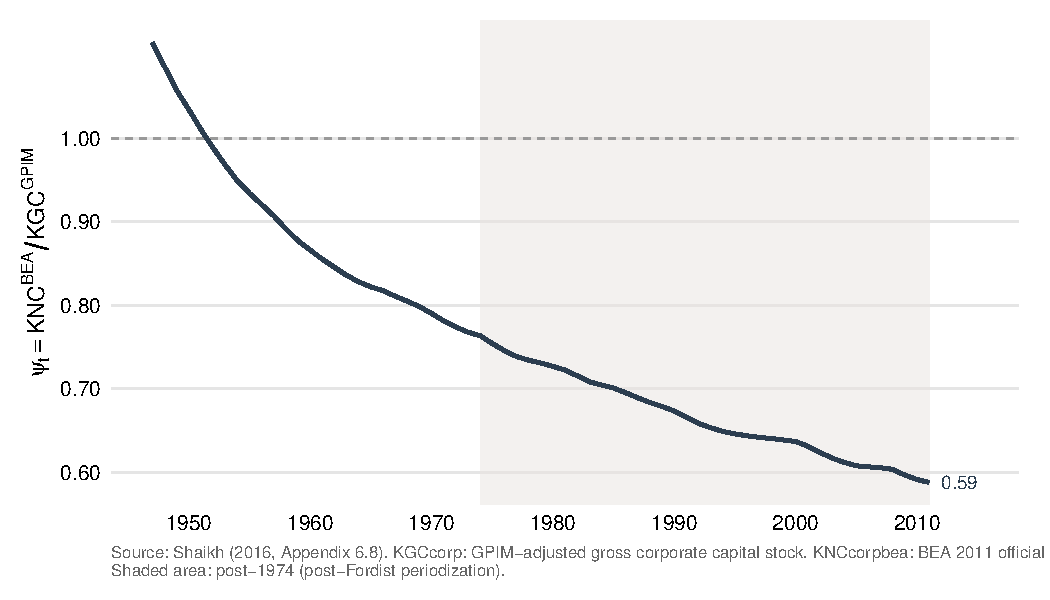
\includegraphics[width=\textwidth]{figures/fig_net_to_gross_ratio.pdf}
\end{figure}

Shaikh's GPIM construction departs from the BEA official methodology in
three respects, each applied as an input to the recursion rather than as
a correction to existing BEA aggregates: substitution of 1993-vintage
BEA finite service lives for the post-revision geometric depletion
rates, pre-war initial values drawn from IRS balance-sheet data rather
than BEA backward extrapolation, and a Great Depression write-down using
the IRS corporate book-value index over
1925--1947.\footnote{Construction formulas, source-table mapping, and
	depletion-rate provenance are in
	Appendix~\ref{app:data_measurement}. The average ratio of the
	GPIM-generated aggregate stock to the BEA current-cost stock over
	1947--2005 is 99.60\%.} The resulting series ---
$\text{KGCcorp}_t$ (gross) and $\text{KNCcorp}_t$ (net) --- are built
entirely from the GPIM recursion under these inputs. The BEA official
net stock $\text{KNCcorpbea}_t$ enters the replication as a comparison
benchmark, not as a starting point.\footnote{Data objects are drawn
	from Appendix~6.8 of \citet{Shaikh2016}, accessible at the companion
	website \texttt{realeconomicanalysis.com}. The source spreadsheet is
	\texttt{\_Appendix6.8DataTablesCorrected.xlsx}. A data audit verifying
	series alignment is documented at script \texttt{90\_data\_audit.R} in
	the replication repository.}


% ---------------------------------------------------------------
% P3 — Corporate output and the deflator
% ---------------------------------------------------------------

The output series entering the cointegrating regression is corrected
corporate gross value added ($\text{GVAcorp}_t$). The critical
replication works under the constraint of relying solely on the
companion data published alongside \citet{Shaikh2016}: the series
presented in his Appendix~6.8 data tables for gross value added of the
corporate sector are the ones used throughout the replication studies,
so that non-replication findings cannot be attributed to independent
data construction. The common deflator $p_t$ is the implicit price
index $pKN$ derived under GPIM rules from the ratio of the current-cost
to constant-cost net capital stock ($\text{KNCcorp}_t /
\text{KNRcorp}_t$, base $2005 = 100$), constructed by Shaikh in
Appendix~6.8 to sustain stock-flow consistency in detriment of the
quality-adjusted chain-weighted deflators published in BEA Fixed Asset
releases.\footnote{Shaikh's Appendix~6.8 does not explicitly name the
	deflator used in the capacity utilization exercise of
	Appendix~6.7.VI. The identification of $pKN$ as the implicit common
	deflator is an S0 finding, confirmed by structural coefficient
	matching against Shaikh's published Table~6.7.14; see
	\S\ref{subsec:S0_shaikh_replication}.} The transformed series
entering all replication stages are therefore
$y_t \equiv \ln(\text{GVAcorp}_t / p_t)$ and
$k_t \equiv \ln(\text{KGCcorp}_t / p_t)$, where $p_t$ is motivated by
the common-deflator rule of \S\ref{subsec:shaikh_id_strategy}.n.
%==================================================================
% §1.4.2 — Stage S0: Faithful Replication of the Capacity Benchmark
% =================================================================

\subsection{Stage S0: Faithful Replication of the Capacity Benchmark}
\label{subsec:S0_shaikh_replication}

This critical replication develops four replication studies, departing from  
Study~S0, which subjects Shaikh's ARDL(2,4) to its first level of scrutiny:
can his published coefficient table be recovered under current-release data,
and under which variable combination within his own data environment?
The exercise faces an immediate obstacle. Shaikh's Appendix~6.8 does not
document which series correspond to the regression variables for output $y$ and 
capital stock $k$ in Appendix Table~6.7.14. No replication dataset
accompanies the published work. An internal annotation in the
Appendix~6.8 spreadsheet \footnote{Two versions of this spreadsheet can be found at \href{https://www.realecon.org/data}{\texttt{Real Economic Analaysis}} website. Its first publication, and a corrected version which is the one used in this esssay.} ---visible in the worksheet metadata but not in the printed tables---states explicitly that the data underlying the capacity
utilization measurement exercise is not documented.\footnote{The note
	appears in the worksheet header of the \texttt{Appndx~6.8.II.7} tab of
	\texttt{\_Appendix6.8DataTablesCorrected\_REA\_release.xlsx}, which contains
	the adjusted corporate value added and real gross operating surplus series.
	The annotation reads, in substance, that the series used for the capacity
	utilization ARDL estimation in Appendix~6.7 are not tabulated in
	Appendix~6.8.} The replicator must therefore reconstruct the specification
from indirect evidence---coefficient magnitudes, fit statistics, and the
long-run multiplier denominator~$(1 - \Sigma\hat{\gamma}_i)$.



A further opacity concerns the deflator. Shaikh advocates a common-deflator
rule throughout \emph{Capitalism}: both output and capital are deflated by
the same price index to preserve profit-rate consistency and eliminate the
relative price channel between output goods and capital goods
\citep[Appendix~6.6]{Shaikh2016}. Yet his Appendix~6.8 workbook contains
no output-side price deflator---no GDP implicit price deflator, and no reference to 
BEA NIPA Table~1.1.9 (the standard source for the GDP deflator at the Bureau of Economic Analysis of the United States). 
A systematic search of all worksheets, including hidden rows and columns, 
confirms that the workbook provides only two candidate price indices: $p^{IG}$, 
the implicit deflator of corporate gross investment, and $p^{KN}$, the implicit deflator of the GPIM-adjusted net
capital stock.\footnote{The search was done manually by the researcher, and assisted by the AI to code a exhaustive search using \texttt{openpyxl} in python to extract all non-empty string cells from the first eight columns of every worksheet, including hidden rows.} The replication
therefore proceeds iteratively across all logically available combinations
of output measure, capital stock concept, and deflator, as reported in full
in Appendix Tables~\ref{tab:S0_candidates_trend}
and~\ref{tab:S0_candidates_notrend}.

Table~\ref{tab:S0_table1} presents the result of that search alongside
Shaikh's published coefficients. The closest replication---candidate C3,
using $y_t = \ln(\text{GVAcorp}_t / p^{KN}_t)$ and
$k_t = \ln(K^G_t / p^{KN}_t)$ without a deterministic trend---matches
Shaikh's two primary diagnostics within rounding: the long-run multiplier
denominator $1 - \Sigma\hat{\gamma}_i = 0.096$ against his published
$0.095$, and RMSE~$= 0.017$ against his $0.016$. More strikingly, the
short-run capital-stock lag pattern---alternating in sign across L0 through
L4 at magnitudes of the same order as Shaikh's $(4.38,\,-11.75,\,
12.39,\,-6.35,\,1.41)$ versus $(5.09,\,-14.28,\,15.71,\,-8.30,\,1.85)$---is
reproduced structurally by no other candidate combination. The dummy
effect for 1974 matches exactly: $\hat{\delta}_{d74} = -0.081^{***}$
in both columns.


%%%% Table 1 %%%%%%%%%%
% =============================================================================
% TABLE: S0 Main — Shaikh vs. C3 Replication (cbind layout, v3)
% LR multipliers include delta-method significance stars
% Denominator note rewritten in terms of AR persistence
% =============================================================================

\begin{table}[htbp]
	\centering
	\small
	\caption{ARDL(2,4) Faithful Replication:
		Shaikh (2016) and Closest Replication}
	\label{tab:S0_table1}
	\begin{threeparttable}
		\begin{tabular}{l r r @{\hspace{2.2em}} l r r}
			\toprule
			& \multicolumn{2}{c}{\textit{Short-run coef.}}
			& & \multicolumn{2}{c}{\textit{Long-run \& fit}} \\
			\cmidrule(lr){2-3} \cmidrule(lr){5-6}
			& Shaikh & Repl.\
			& & Shaikh & Repl.\ \\
			& (2016) & C3
			& & (2016) & C3 \\
			\hline\hline
			%
			$L_1 y_t$
			& $ 1.298^{***}$ & $ 1.242^{***}$
			& $1 - \Sigma\gamma$
			& $0.095$ & $0.096$ \\
			%
			$L_2 y_t$
			& $-0.393^{***}$ & $-0.338^{**\phantom{*}}$
			& $\hat{\theta}$
			& $0.661$ & $0.720^{***}$ \\
			%
			&  &
			& $\hat{a}$
			& $2.178$ & $0.570\phantom{^{***}}$ \\[3pt]
			%
			$k_t\;(L_0)$
			& $ 5.086^{***}$ & $ 4.378^{***}$
			& $d_{1956}$ (LR)
			& $-0.743$ & $-0.649^{**\phantom{*}}$ \\
			%
			$L_1 k_t$
			& $-14.285^{***}$ & $-11.754^{***}$
			& $d_{1974}$ (LR)
			& $-0.855$ & $-0.841^{**\phantom{*}}$ \\
			%
			$L_2 k_t$
			& $15.705^{***}$ & $12.386^{***\phantom{}}$
			& $d_{1980}$ (LR)
			& $-0.478$ & $-0.456^{**\phantom{*}}$ \\[3pt]
			%
			$L_3 k_t$
			& $-8.296^{***}$ & $-6.350^{***}$
			& $R^2$
			& $0.9992$ & $0.9993$ \\
			%
			$L_4 k_t$
			& $ 1.853^{**\phantom{*}}$ & $ 1.409^{*\phantom{**}}$
			& Adj.\ $R^2$
			& $0.9990$ & $0.9991$ \\[3pt]
			%
			$d_{1956}$
			& $-0.071^{***}$ & $-0.062^{***}$
			& RMSE
			& $0.016$ & $0.017$ \\
			%
			$d_{1974}$
			& $-0.081^{***}$ & $-0.081^{***}$
			& $N$
			& $61$ & $61$ \\
			%
			$d_{1980}$
			& $-0.045^{**\phantom{*}}$ & $-0.044^{*\phantom{**}}$
			&  &  &  \\
			%
			Constant
			& $ 0.207^{**\phantom{*}}$ & $ 0.055^{.\phantom{***}}$
			&  &  &  \\
			%
			\bottomrule
		\end{tabular}
		\begin{tablenotes}
			\footnotesize
			\item $^{***}p{<}0.01$, $^{**}p{<}0.05$, $^{*}p{<}0.10$.
			\item \textit{Notes:}
			$y_t \equiv \ln(\text{GVAcorp}_t / p^{KN}_t)$;
			$k_t \equiv \ln(K^G_t / p^{KN}_t)$,
			where $K^G$ is the GPIM-adjusted gross corporate capital stock
			(Appendix~\ref{app:data_measurement}),
			$p^{KN}_t \equiv \text{KNCcorp}_t/\text{KNRcorp}_t \times 100$
			(Appendix Table~6.8.II.1, \citealt{Shaikh2016}). 
			\item \textit{Dummies:} impulse (value 1 in break year only).
			\item \textit{Long-run multipliers:} $\hat{\theta} = \Sigma\hat{\varphi}_j/(1-\Sigma\hat{\gamma}_i)$
			and $\hat{d}_\text{year} \, \hat{\delta}_h/(1-\Sigma\hat{\gamma}_i)$;
			standard errors via the delta method \citep{Pesaran2001}. 
			\item Full candidates matrix available in the Appendix \S \ref{app:critical_replication_results_extended}, Tables~\ref{tab:S0_candidates_notrend}--\ref{tab:S0_candidates_trend}.
		\end{tablenotes}
	\end{threeparttable}
\end{table}

The structural match confirms that Shaikh's implicit common deflator is
$p^{KN}$, the ratio of his GPIM-adjusted current-cost net stock to its
constant-cost equivalent. This is an internal construction, not an
externally imported price series, and it is documented only within the
capital construction tables of Appendix~6.8.II.1.

Long-run multipliers reported in Panel~B are estimated as ratios whose
denominator, $1 - \Sigma\hat{\gamma}_i$, is the complement of output's
own long-run self-multiplier: a unit impulse to $y_t$ today accumulates
to $1/(1-\Sigma\hat{\gamma}_i)$ units in the long run through the
autoregressive feedback, so at $1 - \Sigma\hat{\gamma}_i = 0.096$ each
period's output shock amplifies approximately tenfold before dissipating.
Standard errors are computed via the delta method \citep{Pesaran2001};
the proximity of the denominator to zero places the system near the unit
root boundary, making these standard errors conservative lower bounds on
true long-run uncertainty. Shaikh (2016) does not report standard errors
for long-run multipliers. Under the replication, $\hat{\theta} = 0.720$
is significant at the 1\% level ($t = 11.8$), and all three dummy
long-run effects are significant at the 5\% level.

Despite the structural match, a residual gap in the point estimate of the
long-run elasticity remains: $\hat{\theta} = 0.720$ against Shaikh's
published $0.661$.
Two sources account for this. First, Shaikh's workbook carries a corrected
release of Appendix~6.8 that post-dates the original publication; an
internal note in the spreadsheet indicates that the corrected tables revise
capital stock levels and depreciation rate assumptions relative to the
original release. The original ARDL estimation was in all probability
performed on the pre-correction vintage, for which the capital stock series
carries a different initial value and depletion-rate path. Second, Shaikh
does not report the canonical initial gross capital stock value
$K^G_{1947}$; the replication uses $170.58$~Bn, but any departure from
Shaikh's undisclosed value propagates through the GPIM recursion into
every subsequent period's capital stock and thereby into the ARDL
coefficients.

A final note concerns the deterministic trend. Shaikh does not discuss
the exclusion of a trend term in Appendix~6.7, despite having introduced
an autonomous component in his theoretical exposition of the capacity
function \citep[ch.~6]{Shaikh2016}. The reason for its absence is
empirically transparent: across every deflator and capital-stock
combination, the trend is either statistically insignificant or---when
the deflator introduces its own secular path---produces catastrophic
collinearity with $\ln K_t$, collapsing $\hat{\theta}$ to negative values
(see Appendix Table~\ref{tab:S0_candidates_trend}). The only candidate
where the trend is negligible and its sign is economically incoherent
($\hat{b} = -0.001$, $t = -0.44$) is the specification that otherwise
best matches Shaikh's published result: C3 with $p^{KN}$ and $K^G$.
The trend exclusion is therefore not an arbitrary design choice but a
restriction enforced by the data under the correct variable specification.

\subsubsection{S0 Results: Bounds Test Evidence and Admissibility}
\label{subsec:S0_bounds}

The faithful replication established that Shaikh's ARDL(2,4) recovers
a long-run multiplier $\hat{\theta} = 0.720$ on C3 data, with denominator
$1 - \Sigma\hat{\gamma}_i = 0.096$ matching his published diagnostic within
rounding. What the replication does not establish is whether his
specification is admissible under proper bounds testing as proposed by \citet{Pesaran2001}. 
Neither under which deterministic closure, Shaikh's claim of presenting evidence on co-integration survives at all. Table~\ref{tab:S0_table2} addresses this. Three specifications are
evaluated: Shaikh's fixed ARDL(2,4), and the winners from the information criteria contest using standard BIC and AIC. In his methodology, Shaikh claims preferring AIC selection criteria, which rewards fitness in deteriment of parsimoiny as BIC does, nevertheless none of them choose his lag-order specification.   

% =============================================================================

\begin{table}[htbp]
	\centering
	\caption{PSS Bounds Test: Shaikh's ARDL(2,4) and IC-Preferred Specifications}
	\label{tab:S0_table2}
	\begin{threeparttable}
		\small
		\begin{tabular}{l l r r r r r l}
			\toprule
			Specification & Case & Stat & $I(0)$ & $I(1)$ & $p$(exact) & $p$(asymp) & Verdict \\
			\hline\hline \\			%
			% Panel A: F-bounds test
			%
			\multicolumn{8}{l}{\textit{Panel A: F-bounds test} $\bigl(H_0:\, \lambda_y = \lambda_k = 0\bigr)$} \\[5pt]
			%
			\textbf{Shaikh ARDL(2,4)}
			%
			& 1~(no const.)    & $3.35$ & $2.47$ & $3.33$ & $0.099$ & $0.092$ & \textbf{CI}$^{\dagger}$ \\
			& 2~(restr.\ int.) & $3.27$ & $3.14$ & $3.64$ & $0.142$ & $0.128$ & ? \\
			& 3~(unres.\ int.) & $4.90$ & $4.16$ & $4.93$ & $0.102$ & $0.093$ & ? \\[4pt]
			%
			BIC winner ARDL(2,3)
			& 1~(no const.)    & $2.89$ & $2.47$ & $3.35$ & $0.145$ & $0.136$ & ? \\
			& 2~(restr.\ int.) & $2.15$ & $3.16$ & $3.64$ & $0.381$ & $0.373$ & no \\
			& 3~(unres.\ int.) & $3.19$ & $4.12$ & $4.91$ & $0.287$ & $0.289$ & no \\[4pt]
			%
			AIC winner ARDL(3,3)
			& 1~(no const.)    & $3.87$ & $2.49$ & $3.34$ & $0.066$ & $0.060$ & \textbf{CI} \\
			& 2~(restr.\ int.) & $2.83$ & $3.15$ & $3.63$ & $0.210$ & $0.199$ & no \\
			& 3~(unres.\ int.) & $4.24$ & $4.14$ & $4.90$ & $0.155$ & $0.146$ & ? \\[4pt]
			%
			% Panel B: t-bounds test
			%
			\midrule
			\multicolumn{8}{l}{\textit{Panel B: $t$-bounds test
					$\bigl(H_0:\, \lambda_y = 0\bigr)$}} \\[3pt]
			Shaikh ARDL(2,4)
			& 1~(no const.)    & $-2.51$ & $-1.62$ & $-2.27$ & $0.062$ & $0.060$ & \textbf{CI} \\
			& 3~(unres.\ int.) & $-2.48$ & $-2.58$ & $-2.93$ & $0.218$ & $0.220$ & no \\[4pt]
			%
			BIC winner ARDL(2,3)
			& 1~(no const.)    & $-2.32$ & $-1.60$ & $-2.26$ & $0.088$ & $0.089$ & \textbf{CI} \\
			& 3~(unres.\ int.) & $-2.25$ & $-2.57$ & $-2.92$ & $0.299$ & $0.307$ & no \\[4pt]
			%
			AIC winner ARDL(3,3)
			& 1~(no const.)    & $-2.74$ & $-1.62$ & $-2.28$ & $0.040$ & $0.036$ & \textbf{CI} \\
			& 3~(unres.\ int.) & $-2.67$ & $-2.60$ & $-2.95$ & $0.164$ & $0.160$ & ? \\
			%
			\bottomrule
		\end{tabular}
		\begin{tablenotes}
			\footnotesize
			\item \textit{Notes:}
			$I(0)$ and $I(1)$ are exact finite-sample critical values at 10\%,
			simulated at $T=65$, $k=1$, with $R=40,000$ bootstrap replications.
			\item \textit{H testing:} \textbf{CI} = statistic exceeds $I(1)$, null rejected;
			\textbf{?} = inconclusive region $[I(0), I(1)]$;
			\textbf{no} = below $I(0)$, null not rejected.
			Case~1 uses a no-constant model. 
			\item \textit{\citet{Pesaran2001} cases:} Cases~2--3 use the constant model. The $t$-bounds test is not defined for Case~2. Exact and asymptotic $p$-values differ by less than $0.01$.
			\item \textit{ARDL specification:} BIC and AIC winners are chosen from grid search of a set of ARDL models under standard search algorithms \citep{Natsiopoulos2024}, variables included in the model are the same than in \ref{tab:S0_table1}).
		\end{tablenotes}
	\end{threeparttable}
\end{table}


The findings partition sharply by case, not by specification. Cases~2
and~3 fail for every specification at every conventional significance level:
the strongest result is Shaikh's ARDL(2,4) under Case~3
($F = 4.90$, $p = 0.102$), which falls just below the $I(1)$ upper bound
($4.93$) and remains inconclusive. Case~1 --- no intercept, no drift, the
closure closest to the unbalanced growth formulation of
\S\ref{sec:conceptual_framework} and further detailed in the appendix \S\ref{app:accumulation_dynamics} --- is the only case where evidence of cointegrating can be found . 
The AIC winner ARDL(3,3) produces the strongest F-bound statistic 
($F = 3.87 > I(1) = 3.34$, $p = 0.066$); Shaikh's ARDL(2,4)
follows marginally ($F = 3.35 > I(1) = 3.33$, $p = 0.099$); the BIC
winner ARDL(2,3) sits in the inconclusive region ($F = 2.89$,
$I(0) = 2.47$, $I(1) = 3.35$). The $t$-bounds test reinforces this
pattern: all three specifications produce CI verdicts under Case~1, with
the AIC winner achieving 5\% significance ($t = -2.74$, $p = 0.040$),
while Case~3 fails for all three.

The partition carries a precise theoretical implication. Case~1 is the
closure the unbalanced growth framework motivates: output and capital
cointegrate around zero in log space, with no autonomous level governing
the long-run trajectory. Case~2 --- under which Shaikh's demeaning
normalization $\hat{u}_t = \exp(\text{ECT}_t - \overline{\text{ECT}})$
is internally coherent, because a restricted intercept ensures the ECT has
a stable mean --- finds no cointegrating evidence anywhere in the data.
The specification that makes the normalization valid is the one the data
rejects; the specification under which cointegration survives produces a
different long-run equation from the one Shaikh's normalization presupposes.

A final observation concerns Shaikh's reported bounds test. The
$F(10, 50) = 6257$ statistic in Appendix Table~6.7.14 of
\citet{Shaikh2016} is the standard OLS goodness-of-fit test --- the joint
null that all coefficients are zero --- not the PSS bounds test, which
examines the 2-restriction null $H_0: \phi_1 = \phi_2 = 0$ on the lagged
levels in the ECM reparameterization \citep{Pesaran2001}. Shaikh declares
no PSS case and evaluates the wrong test statistic. The cointegrating
evidence he claims has no valid inferential basis as reported.



% =============================================================================
% S0 CLOSURE — FINAL (v2)
% Figure placement + What S0 Establishes
% For insertion at end of §4.2 (Stage S0: Faithful Replication)
% =============================================================================

% ── Figure ───────────────────────────────────────────────────────────────────

\begin{figure}[htbp]
	\centering
	\caption{Capacity utilization (1947--2011): Alternative Measures.}
	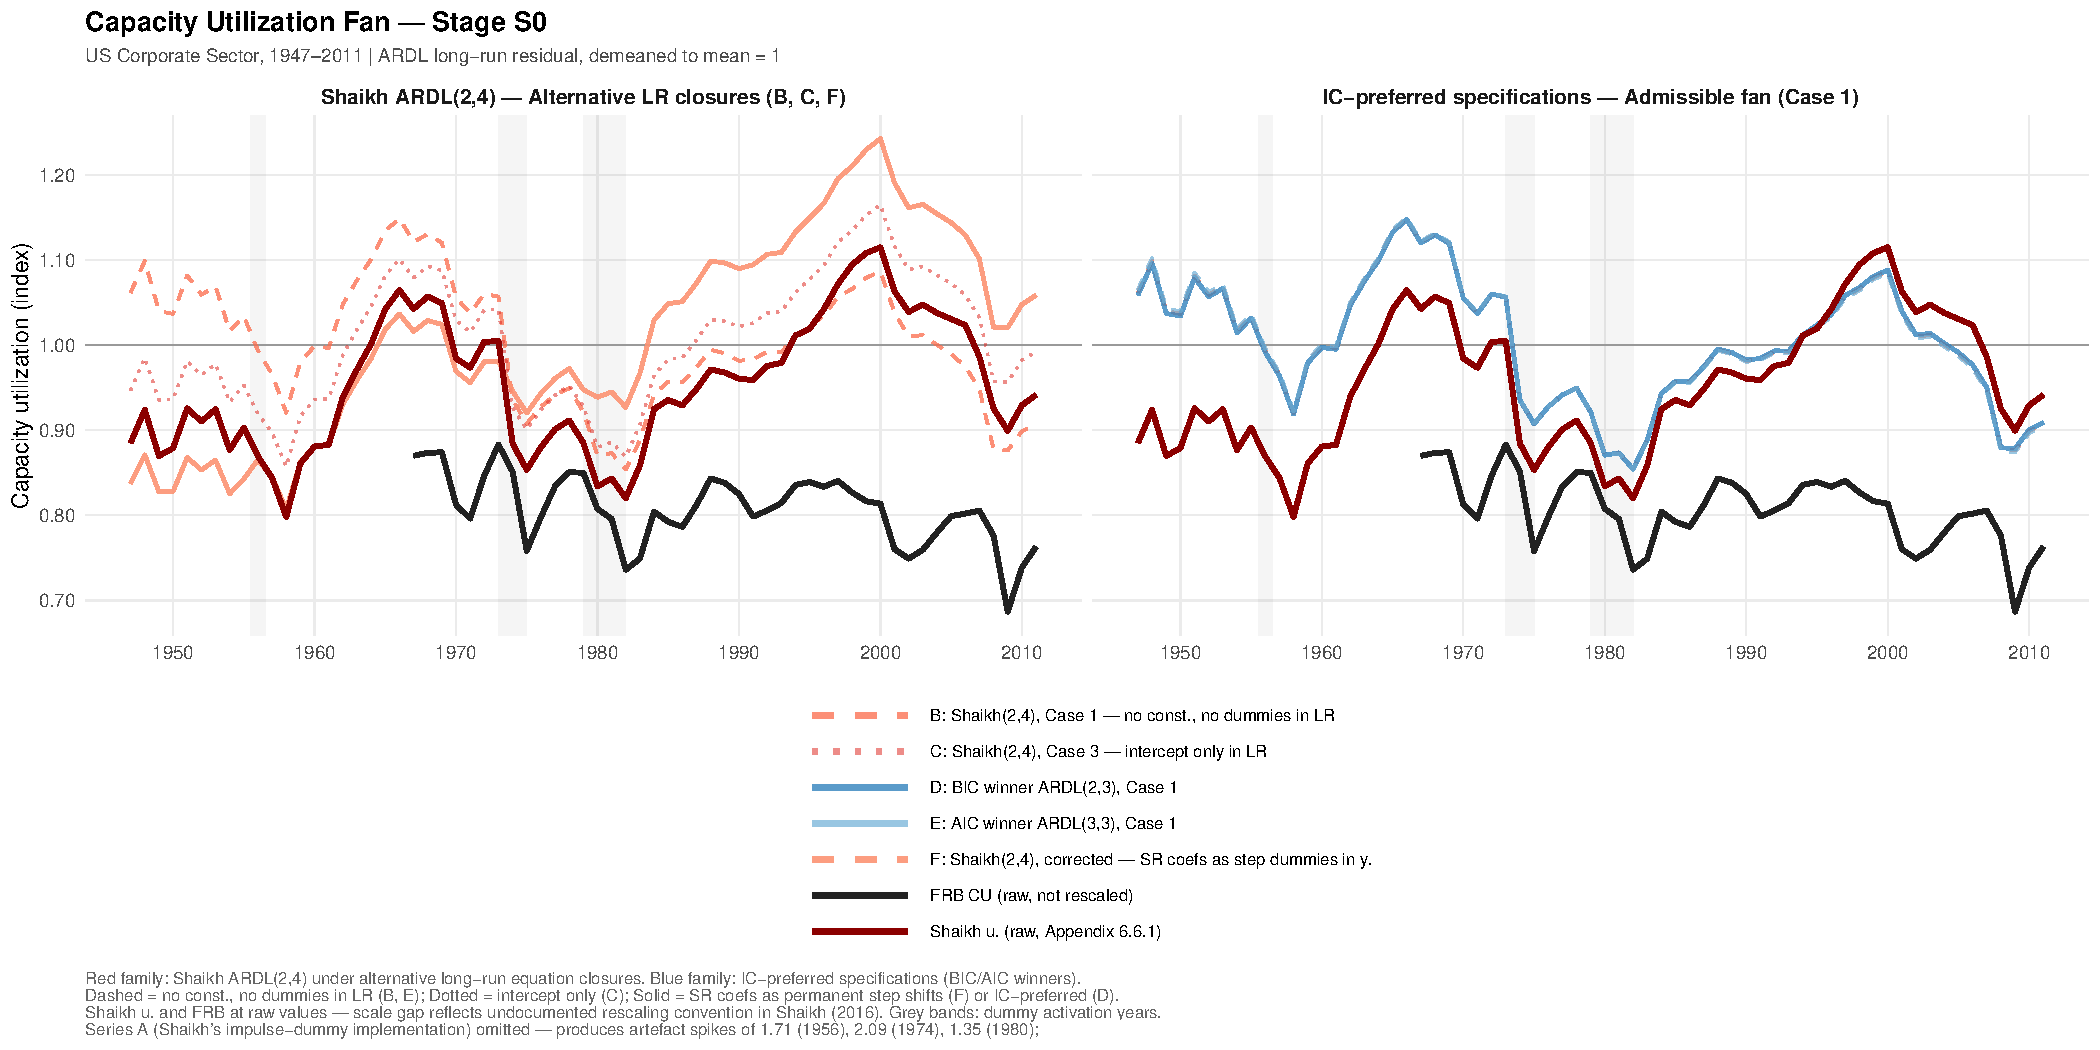
\includegraphics[width=\textwidth]{figures/fig_S0_cu_fan.pdf}
	\label{fig:S0_cu_fan}
\end{figure}


% ── What S0 Establishes ──────────────────────────────────────────────────────

\subsubsection{What S0 Establishes}
\label{subsubsec:S0_establishes}

The deflator implicit in Shaikh's workbook is $p^{KN}$---an internal
GPIM construction, not an externally imported price series. The
closest variable combination (C3:
$y_t = \ln(\text{GVAcorp}_t/p^{KN}_t)$,
$k_t = \ln(K^G_t/p^{KN}_t)$, no trend) recovers his two primary
diagnostics within rounding
($1-\Sigma\hat{\gamma}_i = 0.096$; RMSE~$= 0.017$). The trend is
excluded by the data: across every variable combination a significant
trend collapses $\hat{\theta}$ to negative values through collinearity
with $k_t$. The residual gap in $\hat{\theta}$ ($0.720$ against
$0.661$) is attributable to a post-publication correction and the
undisclosed initial capital stock value---data vintage, not
specification error.

Admissibility fails on Shaikh's own terms. The $F(10,50)=6257$ he
reports is the OLS goodness-of-fit statistic, not the PSS
2-restriction bounds test \citep{Pesaran2001}; he declares no
deterministic case. Under proper testing, cointegration survives only
under Case~1 ($F = 3.35 > I(1) = 3.33$; $t = -2.51$, $p = 0.062$),
where the AIC winner ARDL(3,3) delivers stronger evidence than
Shaikh's own specification ($F = 3.87$; $p = 0.040$). The
specification that makes the normalization valid---Case~2, where the
restricted intercept gives the ECT a stable mean---is the one the
data rejects. The specification under which cointegration
survives produces a different long-run equation from the one Shaikh's
normalization presupposes.

The evidence favors an unbalanced growth closure with $\hat{\theta}
< 1$, but the stabilizing force is not endogenous to the
specification: the accounting dynamics derived in
Appendix~\S\ref{app:accumulation_dynamics} admit no interior
attractor under the classical long-run closure when $\theta \neq 1$.
Whether an alternative ARDL specification resolves these caveats,
whether system-level estimation recovers a more robust identification,
and whether the scalar $\theta$ masks regime variation across
accumulation regimes---these are the questions the subsequent stages
address.

% =============================================================================
% §1.4.4 Stage S1 — ARDL Specification Geometry
% Figure: fig_S1_ic_tangencies (H placement, main text)
% Appendix refs: fig_S1_global_frontier, fig_S1_informational_domain
% =============================================================================


\subsection{Stage S1: ARDL Specification Geometry}
\label{subsec:S1}

S0 leaves Q1 open: is the ARDL(2,4) failure idiosyncratic to Shaikh's
lag order, or structural to the single-equation framework? S1 answers
by exhausting the admissible ARDL space on C3 data. The specification
grid covers $p, q \in \{1,\ldots,5\}$, all five PSS deterministic
cases, and four dummy structures
$s \in \{s_0, s_1, s_2, s_3\}$,\footnote{%
	$s_0$: no dummies; $s_1$: $d_{1974}$ only; $s_2$: $d_{1974}$,
	$d_{1980}$; $s_3$: $d_{1956}$, $d_{1974}$, $d_{1980}$ (Shaikh's
	structure). Each dummy is an impulse indicator taking the value 1
	in the break year only.}
yielding 500 candidate specifications. Of these, 100 fail estimation
--- all corresponding to Cases~4--5 on no-trend models, which the
estimator correctly rejects as structurally incompatible. The remaining
400 are estimated and submitted to the admissibility gate. Formally:
\begin{equation}
	\label{eq:G_S1}
	\mathcal{G}_{S1} \;=\;
	\bigl\{\,(p,\, q,\, c,\, s)\,\bigr\}
\end{equation}

Admissibility is defined by the PSS $F$-bounds test: a specification
enters the admissible set $\mathcal{A}_{S1} \subseteq \mathcal{G}_{S1}$
if and only if the $p$-value of the joint null
$H_0: \lambda_y = \lambda_k = 0$ satisfies $p \leq 0.10$.
Critical values are asymptotic values provided by \citet{Pesaran2001},
rather than the exact finite-sample values used at S0 ($T = 65$);
asymptotic critical values are uniformly less conservative, making
$\mathcal{A}_{S1}$ an upper bound on what finite-sample testing would
deliver.\footnote{%
	Under the exact PSS simulation used in S0, Cases~2 and~3 failed
	entirely for Shaikh's specification; under asymptotic critical values,
	Cases~2 and~3 contribute 6 specifications each to the frontier.
	The discrepancy is methodologically consequential and reported for
	transparency.}
Of 400 estimable specifications, 65 pass the gate, constituting
$\mathcal{A}_{S1}$.

Within $\mathcal{A}_{S1}$, model selection proceeds through the
fit--complexity plane $(k(m),\; -2\log L(m))$, where $k(m)$ is the
total parameter count --- interpreted as model \emph{complexity} ---
and $-2\log L(m)$ is the negative log-likelihood, where lower values
indicate higher fit. The Pareto envelope $\mathcal{E}_{S1}$ selects,
at each complexity level $k$, the specification in $\mathcal{A}_{S1}$
with the highest log-likelihood:
\begin{equation}
	\label{eq:E_S1}
	\mathcal{E}_{S1}(k) \;=\;
	\arg\max_{m \,\in\, \mathcal{A}_{S1},\; k(m)=k}
	\;\log L(m)
\end{equation}
With 17 distinct values of $k$ represented in $\mathcal{A}_{S1}$,
$\mathcal{E}_{S1}$ contains 17 specifications spanning $k=5$ to
$k=15$ --- one Pareto-dominant specification at each complexity
level.\footnote{%
	A fattened frontier $\mathcal{F}^{(0.20)}$ was also constructed,
	defined as the set of admissible specifications whose vertical
	distance from $\mathcal{E}_{S1}$ at their own $k$ falls in the
	bottom $20\%$ of the distance distribution across $\mathcal{A}_{S1}$.
	Since $26\%$ of admissible specifications ($17$ of $65$) sit
	directly on the envelope ($\delta = 0$), the 20th percentile of
	the distance distribution is exactly zero, and
	$\mathcal{F}^{(0.20)} = \mathcal{E}_{S1}$ in this dataset.
	The fattening exercise is therefore vacuous here and
	$\mathcal{E}_{S1}$ is retained as the reference object throughout.
	The Pareto envelope and the admissible cloud are shown in
	Appendix Figures~\ref{fig:S1_global_frontier} and
	\ref{fig:S1_informational_domain}.}
Information criteria appear as iso-penalty contours over this plane
with slopes set by their complexity penalty: AIC with slope $2$, BIC
with slope $\ln T$, and HQ with slope $2\ln\ln T$; ICOMP and RICOMP
penalize parameter interdependence through the Fisher information
matrix and produce non-linear contours. The tangency of each contour
with $\mathcal{E}_{S1}$ identifies the IC winner for that criterion.

\begin{figure}[H]
	\centering
	\caption{IC tangency points in the ARDL fit--complexity plane}
	\label{fig:S1_ic_tangencies}
	
\includegraphics[width=\textwidth]{figures/fig_S1_ic_tangencies.pdf}
	\begin{minipage}{\textwidth}
		\footnotesize
		\textit{Notes:}
		\begin{itemize}[leftmargin=1em, itemsep=0pt, topsep=2pt]
			\item Each point is an admissible specification ($n = 65$,
			PSS $F$-bounds gate $p \leq 0.10$, asymptotic critical
			values, $T = 65$). The dark envelope traces
			$\mathcal{E}_{S1}$.
			\item Blue asterisk~($*$): Shaikh's $m_0 = (2,4,c_3,s_3)$,
			inadmissible under proper PSS case discipline, coinciding
			with the HQ tangency point.
		\end{itemize}
	\end{minipage}
\end{figure}

Figure~\ref{fig:S1_ic_tangencies} represents the specification geometry
of ARDL models on Shaikh's data. Dashed lines are IC iso-penalty
contours: BIC/ICOMP/RICOMP (steeper, heavier penalty) and AIC/HQ
(shallower, lighter penalty). Information criteria winner symbols mark
the tangency points: BIC, ICOMP, and RICOMP converge on
ARDL(1,2,$c_2$,$s_0$) at $k=5$; HQ selects ARDL(5,3,$c_2$,$s_1$)
at $k=11$; AIC selects ARDL(5,4,$c_2$,$s_1$) at $k=12$.

The criteria split into two families, visible in the figure as two
distinct clusters along the envelope. At $k=5$, BIC, ICOMP, and RICOMP
converge on ARDL(1,2,$c_2$,$s_0$) --- the most parsimonious admissible
specification, with no dummies and a restricted intercept,
$\hat{\theta} = 0.651$. They arrive there from distinct directions.
BIC penalizes over-fitting through a raw parameter count: each
additional parameter costs $\ln T \approx 4.17$ units at $T=65$,
regardless of what the parameter does. ICOMP operates differently: it
penalizes parameter \textit{interdependence} by measuring the entropic
complexity of the inverse Fisher information matrix. When the
eigenvalues of $\hat{F}^{-1}$ are unequal --- that is, when parameter
estimates are correlated --- the ICOMP penalty fires. Under the near
unit-root AR dynamics of this data
($1 - \Sigma\hat{\gamma}_i \approx 0.096$), adding AR lags produces
strongly collinear parameter estimates, inflating eigenvalue dispersion
and triggering a heavy ICOMP penalty on longer-lag specifications.
RICOMP applies the same complexity measure to the sandwich covariance
matrix, making it robust to heteroskedasticity while preserving this
sensitivity to collinearity. That all three converge on $k=5$ ---
through parameter count, parameter correlation, and robust parameter
correlation respectively --- is a stronger indictment of longer-lag
models than any single criterion could deliver alone. Their iso-penalty
contours are steep enough that any move rightward along the envelope
is more than offset by the added complexity cost, making $k=5$ the
unambiguous minimum under heavy penalization. At $k=11$--$12$, AIC
and HQ tell a different story. With shallower penalty slopes, they
remain sensitive to fit gains even where the frontier is already flat,
selecting specifications with five AR lags and the $d_{1974}$ dummy,
$\hat{\theta} \approx 0.849$--$0.857$. Three distinct winners emerge
across five criteria: the selected specification is an artefact of the
researcher's implicit criterion prior, not a property identified by
the data.

Shaikh's specification $m_0 = (2,4,c_3,s_3)$ --- marked by the blue
asterisk --- coincides with the HQ tangency point at $k=11$, suggesting
his lag selection implicitly minimized the Hannan-Quinn criterion,
though he documents no selection procedure. Despite this near-optimality
under HQ, $m_0$ fails the admissibility gate: it produces only marginal
cointegration evidence under Case~1 ($F = 3.35$, $p = 0.099$) and
fails entirely under Cases~2 and~3. The IC-preferred AIC winner
ARDL(3,3) produces stronger cointegration evidence on the same
criterion ($F = 3.87$, $t = -2.74$, $p = 0.040$): Shaikh's lag order
is inferior to the IC optimum on his own cointegration criterion.

Across the 17 specifications in $\mathcal{E}_{S1}$, $\hat{\theta}$
ranges from $0.651$ to $2.204$. The outlier at $\hat{\theta} = 2.204$
is ARDL(1,2,$c_4$,$s_3$) --- Case~4 includes a deterministic trend,
which inflates $\hat{\theta}$ explosively through the near-zero
denominator ($1 - \Sigma\hat{\gamma}_i = 0.123$). Restricting to
Cases~2 and~3 --- the econometrically coherent closures established
in S0 --- the 16 remaining envelope specifications produce
$\hat{\theta} \in [0.651, 0.866]$ with mean $0.829$ and standard
deviation $0.060$. The single most consequential researcher degree of
freedom in the ARDL identification of $\hat{\theta}$ is therefore the
deterministic case selection, not the lag order. Shaikh's $m_0$ does
not appear in $\mathcal{A}_{S1}$ and is absent from $\mathcal{E}_{S1}$
entirely.

\subsubsection{What S1 Establishes}
\label{subsubsec:S1_establishes}

The caveats documented in S0 are not incidental to Shaikh's choice of ARDL(2,4)---they are structural to the single-equation framework itself. Exhausting the full admissible grid $\mathcal{A}_{S1}$ across every lag combination, deterministic case, and dummy structure reveals a single dominant pattern: every specification in $\mathcal{A}_{S1}$ inherits three architectural constraints. First, the cointegration rank is fixed at one by construction rather than tested. Second, long-run normalization is imposed on output rather than identified from the data. Third, long-run multipliers must pass through a near-zero denominator $1 - \Sigma\hat{\gamma}_i$, amplifying any specification perturbation. No combination of lag order, dummy structure, or deterministic case resolves these constraints---they are properties of ARDL models as such, not of any particular specification within the class.

Figure~\ref{fig:S1_theta_and_cu_fan} makes this problem
visible from two directions. The left panel shows that $\hat{\theta}$
across $\mathcal{E}_{S1}$ is heavily concentrated in $[0.651, 0.866]$
under Cases~2 and~3 --- the econometrically coherent closures
established in S0 --- with a single outlier at $\hat{\theta} = 2.204$
driven by Case~4's trend interaction with the near-zero denominator.
Shaikh's $m_0$, marked by the dashed blue line at $\hat{\theta} =
0.720$, lies to the left of the main envelope cluster and below every
Case~2 or~3 envelope specification. The knife-edge at $\hat{\theta}
= 1$ separates the overaccumulation regime ($\hat{\theta} < 1$,
demand face of investment exceeds capacity face) from the
underaccumulation regime ($\hat{\theta} > 1$). Every
Cases~2--3 envelope specification falls below the knife-edge,
confirming overaccumulation as a structural property of the admissible
ARDL grid, not a feature of any particular lag order. The long-run tendency toward over-accumulation of accumulation demand in the U.S.\ corporate sector is a qualitative invariant of the specification family---every admissible ARDL specification recovers $\hat{\theta} < 1$---but the magnitude of $\hat{\theta}$ is determined by the researcher's criterion prior, not by the data.


\begin{figure}[H]
	\centering
	\caption{$\hat{\theta}$ distribution and capacity utilization fan
		across $\mathcal{E}_{S1}$ (Pareto envelope)}
	\label{fig:S1_theta_and_cu_fan}
	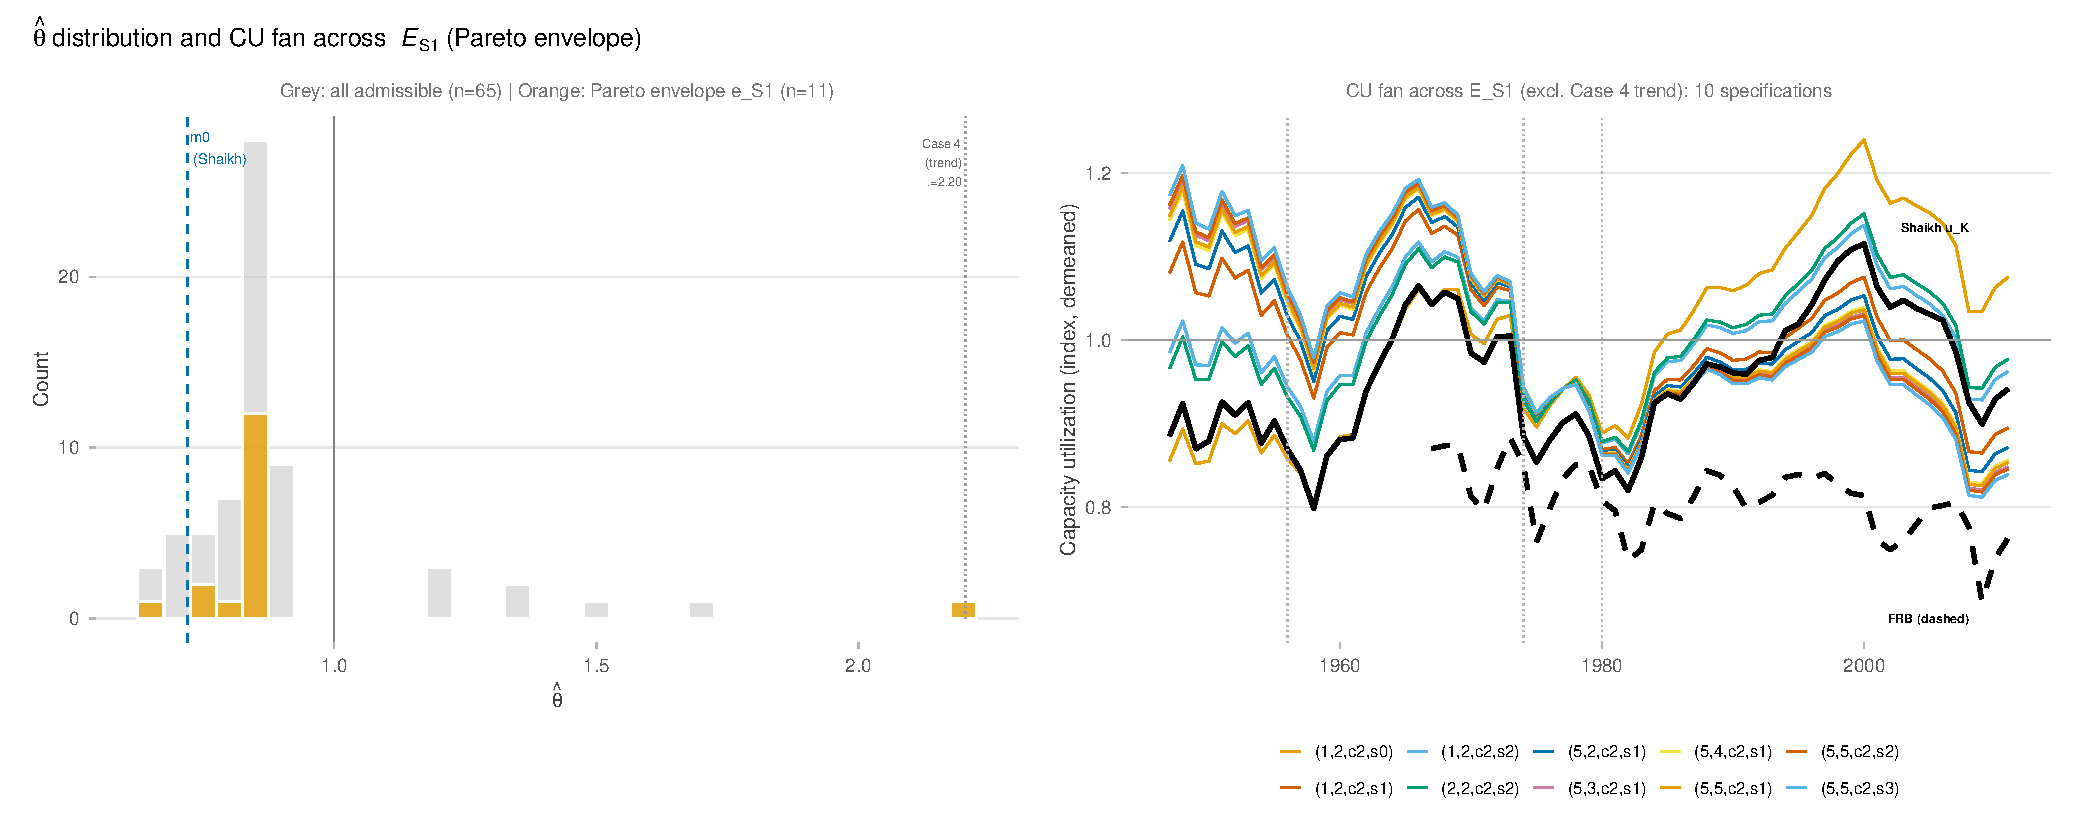
\includegraphics[width=\textwidth]{figures/fig_S1_theta_and_cu_fan}
	\begin{minipage}{\textwidth}
		\footnotesize
		\textit{Notes:}
		\begin{itemize}[leftmargin=1em, itemsep=0pt, topsep=2pt]
			\item \textit{Left panel}: $\hat{\theta}$ histogram across
			$\mathcal{A}_{S1}$ (grey) and Pareto envelope
			$\mathcal{E}_{S1}$ (orange). Dashed blue line: Shaikh's
			$\hat{\theta}_{m_0} = 0.720$. Solid vertical: knife-edge
			$\hat{\theta} = 1$. The lone orange bar at $\hat{\theta}
			= 2.204$ is ARDL(1,2,$c_4$,$s_3$) --- Case~4 includes a
			deterministic trend, inflating $\hat{\theta}$ through the
			near-zero denominator.
			\item \textit{Right panel}: CU fan across $\mathcal{E}_{S1}$,
			Case~4 excluded. Color families correspond to lag--dummy
			combinations (see legend). Solid bold: Shaikh's published
			$\hat{u}_K$ (raw). Dashed bold: FRB capacity utilization
			(raw, not rescaled). Grey dotted verticals: dummy activation
			years ($d_{1956}$, $d_{1974}$, $d_{1980}$).
		\end{itemize}
	\end{minipage}
\end{figure}


The right panel shows the consequence in the utilization space. The
CU fan across Cases~2--3 envelope specifications is tight throughout
the sample --- the paths produced by different lag orders and dummy
structures track closely, with visible spread only in the early
period 1947--1960 where the sparse data make the AR dynamics less
constrained. The Shaikh $\hat{u}_K$ benchmark (solid bold) floats
above the fan from the mid-1990s onward, a growing gap that reflects
the normalization problem documented in S0: the published series
requires an undocumented rescaling that no lag order or dummy structure
within the ARDL class can replicate mechanically. The FRB series
(dashed bold) sits approximately 15--20 percentage points below the
fan throughout --- the scale incommensurability is persistent across
every specification in $\mathcal{E}_{S1}$ and is not resolved by any
lag order or dummy structure within the ARDL class.

The IC contest confirms the structural verdict from a different angle.
Three distinct winners emerge across five criteria: BIC, ICOMP, and
RICOMP converge at $k=5$, $\hat{\theta} = 0.651$; HQ and AIC converge
at $k=11$--$12$, $\hat{\theta} \approx 0.849$--$0.857$. Hence, the conclusion is that under ARDL models the magnitude of unbalanced growth is subject to the implicit researcher's criterion prior, without further structural identification. Shaikh's $m_0$ coincides with the HQ tangency point,
suggesting implicit criterion minimization without documentation,
and fails admissibility simultaneously.

S2 moves to the Johansen VECM, which releases all three constraints:
rank is tested via the trace statistic, the full loading vector
$\alpha$ is recovered, and $\hat{\theta}$ is estimated as a system
eigenvector without a near-zero denominator filter. The information
set is simultaneously expanded from $(y_t, k_t)$ to
$(y_t, k_t, e_t)$, where the rate of exploitation
$e_t = \text{Profshcorp}_t / (1 - \text{Profshcorp}_t)$ is
constructed from the corrected corporate profit share documented in
Appendix~\ref{app:data_measurement}. The transformation maps the
profit share from the unit interval onto $[0, \infty)$, encoding
both distributional shares in a single variable whose unbounded
upper support registers the explosive dynamics that a bounded
measure suppresses. The question S2 poses is not whether the VECM
delivers a more robust $\hat{\theta}$, but whether the
capital--output attractor is genuinely bivariate or
distributionally mediated---and, if the latter, what the adjustment
structure reveals about the relation of distributive conflict and our structural parameter of interest $\theta$.


% ============================================================%   Stage S2: System-Level VECM Replication  (compact v3)
% ===========================================================%
% =============================================================================
% §  Stage S2: System-Level VECM Replication  (compact v3)
% =============================================================================

\subsection{Stage S2: System-Level VECM Replication}
\label{sec:S2}

S1 established that $\hat{\theta}$ is stable within the admissible ARDL
class but that its magnitude is governed by the researcher's criterion
prior. Three architectural constraints proved intrinsic to the
single-equation framework: cointegrating rank fixed at $r=1$ by
construction, long-run normalization imposed on output, and near-zero
denominator amplification. S2 asks whether the long-run relation survives
as a system property when these constraints are released.

The Johansen reduced-rank VECM \citep{Johansen1991} releases
all three. Cointegrating rank is tested endogenously via trace and
maximum-eigenvalue statistics---the central methodological innovation
relative to S0--S1, where rank was maintained by construction. The full
loading vector $\alpha$ is recovered, identifying which equations carry the
adjustment burden; and $\hat{\theta}$ is estimated as a system eigenvector
without passing through a near-zero denominator filter. The information set
is simultaneously expanded from $(y_t, k_t)$ to $(y_t, k_t, e_t)$, where
$e_t$ is the rate of exploitation introduced in
\S\ref{subsubsec:S1_establishes}. Two system dimensions are estimated: the
bivariate $m=2$ system $X_t = (\ln Y_t, \ln K_t)'$ reproduces Shaikh's
core structure at the system level; the trivariate $m=3$ system
$X_t = (\ln Y_t, \ln K_t, \ln e_t)'$ tests whether the capital--output
attractor requires distributional information. Under $m=3$, the rank
hypothesis $r=2$ is also testable: a second cointegrating vector would
open the possibility of identifying reserve-army dynamics alongside the
capacity relation.\footnote{Structural identification of two cointegrating vectors would require a
							rotation of the canonical correlation space, such a plausible 
							exploitation--utilization relation, is expressed in terms of the structural 
							relation of productive capacities and effective demand mediated by the structural 
							coefficient $\theta$. This diagnostic is evaluated if and only if $r=2$ specifications 
							enter the admissible set.}

Each candidate $m \in \mathcal{G}_{S2}$ can be represented as follows: 

\begin{equation}
	\label{eq:S2_grid}
	\mathcal{G}_{S2} \;=\;
	\bigl\{\,(m,\, r,\, p,\, d,\, h)\,\bigr\},
\end{equation}
%
where $m \in \{2,3\}$, $r$ is the cointegration rank ($r=1$ for $m=2$;
$r \in \{1,2\}$ for $m=3$), $p \in \{1,\ldots,4\}$ the VAR lag depth,
$d \in \{d_0, d_1, d_2, d_3\}$ the deterministic branch
\citep[ch.~6]{Johansen1995}, and $h \in \{h_0, h_1, h_2\}$ the
step-dummy structure.\footnote{%
	$h_0$: no dummies; $h_1$: step at 1974; $h_2$: steps at 1956, 1974,
	1980. As in S1, these shift the level of the capacity benchmark;
	slope-change diagnostics are deferred to S3.}
The grid yields 144 specifications (48 bivariate, 96 trivariate). Each
implies a reduced-rank VECM:
%
\begin{equation}
	\label{eq:S2_vecm}
	\Delta X_t \;=\; \alpha\beta' X_{t-1}
	\;+\; \sum_{i=1}^{p-1} \Gamma_i \,\Delta X_{t-i}
	\;+\; \text{det}(d,h)
	\;+\; \varepsilon_t,
\end{equation}
%
with $\mathrm{rank}(\alpha\beta') = r$, estimated via maximum likelihood
\citep{Stigler2020, Reinsel2022}.

A specification enters the admissible set $\mathcal{A}_{S2}$ if and only
if it passes three sequential gates. First, the estimator must converge
without producing degenerate or missing coefficients. Second, the Johansen
trace test must reject the null of insufficient rank at the 5\% level---
confirming that the data support the imposed number of cointegrating
relations. Third, the estimated system must be dynamically stable: all
eigenvalues of the companion matrix must lie on or inside the unit circle,
ensuring that the VECM does not imply explosive trajectories. The rank
gate is the decisive filter---it is entirely absent from the ARDL
framework, where cointegrating rank is maintained by construction rather
than tested.

Among admissible specifications, comparison proceeds through the
fit--complexity plane $m \mapsto (k(m),\, {-2\log L}(m))$, where $k(m)$
counts all system parameters. Cross-dimensional comparisons normalize by
$m \cdot T_{\text{eff}}$. The same four information criteria used in S1
(AIC, BIC, HQ, ICOMP) select tangency points along the Pareto
envelope.\footnote{
	RICOMP requires a sandwich covariance matrix unavailable for the VECM
	estimator; it is omitted from S2.}
As in S1, the diagnostic question is whether the tracked
objects---$\beta$, $\hat{\theta}$, $\alpha$, and the utilization series
$\widehat{u}_t$---are stable across the admissible set or vary
systematically with the specification.

% --- S2 Results ---

% =============================================================================
% S2 Results
% =============================================================================

\subsubsection{S2 Results: Admissibility, Rank, and Adjustment Structure}
\label{subsubsec:S2_results}

Table~\ref{tab:S2_admissibility} reports admissibility outcomes across
the full grid $\mathcal{G}_{S2}$. Of 144 specifications, 36 fail
estimation---all corresponding to the $d_1$ branch, which produces
numerical degeneracy under the \texttt{tsDyn} estimator for every
$(p, h)$ combination. Of the 108 that converge, only 6 pass the triple
admissibility gate. All 6 are trivariate ($m=3$) with rank $r=1$.

% =============================================================================
% Table: S2 Admissibility Outcomes
% File: tables/S2_admissibility.tex
% =============================================================================

\begin{table}[htbp]
\centering
\small
\caption{S2 admissibility outcomes across the VECM specification grid}
\label{tab:S2_admissibility}
\begin{threeparttable}
\begin{tabular}{llrrrr}
\toprule
System & Rank & Estimated & \multicolumn{2}{c}{Failed gate} & Admissible \\
\cmidrule(lr){4-5}
       &      &           & Rank & Stability &            \\
\midrule
\multicolumn{6}{l}{\textit{Panel A: Bivariate} ($X_t = (\ln Y,\, \ln K)'$)} \\[4pt]
$m = 2$ & $r = 1$ & 36 & 36 & 4 & \textbf{0} \\[6pt]
\multicolumn{6}{l}{\textit{Panel B: Trivariate} ($X_t = (\ln Y,\, \ln K,\, \ln e)'$)} \\[4pt]
$m = 3$ & $r = 1$ & 36 & 26 & 4 & \textbf{6} \\
$m = 3$ & $r = 2$ & 36 & 29 & 7 & \textbf{0} \\[4pt]
\midrule
\multicolumn{2}{l}{Total} & 108 & 91 & 15 & \textbf{6} \\
\bottomrule
\end{tabular}
\begin{tablenotes}
\footnotesize
\item \textit{Notes:} $\mathcal{G}_{S2}$ contains
    144 candidates. All $d_1$ branch failed feasible estimation leaving 108 estimated. 
    Gate failures are not mutually exclusive: a specification may fail both rank and stability.
    The rank gate requires the Johansen trace test to reject
    $H_0\!: r < r^*$ at 5\%.
    Sample: 1947--2011 ($T = 65$, $T_{\text{eff}} = 63$--$64$).
\end{tablenotes}
\end{threeparttable}
\end{table}


The bivariate system ($m=2$) produces zero admissible specifications.
All 36 estimated bivariate models fail the rank gate: the Johansen trace
test cannot reject $H_0\!: r = 0$ at 5\% for any combination of lag
depth, deterministic branch, or step-dummy structure. This is the most
consequential finding of S2. Under a prior data vintage ($T = 61$,
sample ending in 2007), the same bivariate grid yielded 12 admissible
specifications with $\hat{\theta} \in [0.88, 0.91]$. The four
post-crisis years (2008--2011) erode the bivariate rank evidence below
the trace-test threshold. The bivariate VECM result is sample-fragile:
four observations reverse the cointegration verdict. The ARDL, which
does not require a rank test, survives the same sample extension---a
direct head-to-head robustness comparison between the two frameworks.

The trivariate system with $r = 2$ also produces zero admissible
specifications: the trace test cannot reject $H_0\!: r < 2$ for any of
the 36 estimated models. The data support at most one cointegrating
relation. The structural rotation diagnostic described in
\S\ref{sec:S2}---separating a capacity relation from a reserve-army
relation under the sign restriction $\lambda < 0$---cannot be
evaluated.\footnote{%
	The empty rotation-check file (\texttt{S2\_rotation\_check.csv})
	confirms this: zero $r=2$ specifications survive for the canonical
	correlation decomposition to operate on.}
The exploitation rate contributes to the system's short-run dynamics and
adjustment structure, but does not sustain an independent long-run
attractor alongside the capital--output relation.

% ── Admissible set structure ─────────────────────────────────────

The 6 surviving specifications share a common architecture.
Table~\ref{tab:S2_admissible} reports their key parameters. All require
the full three-shock structure $h_2$ (step dummies at 1956, 1974, 1980);
no specification without all three dummies passes the rank test. This
confirms that structural breaks are load-bearing for cointegration
identification: the long-run relation between output, capital, and
exploitation does not hold as a stable attractor across the full
sample without acknowledging that the institutional substrate shifted
at those dates. Only $p = 1$ and $p = 2$ survive; higher lags consume
degrees of freedom without gaining rank support. The deterministic
branches $d_0$, $d_2$, and $d_3$ all appear.


\begin{table}[htbp]
	\centering
	\small
	\caption{Admissible VECM specifications ($m=3$, $r=1$, $h_2$)}
	\label{tab:S2_admissible}
	\begin{threeparttable}
		\begin{tabular}{lcccrrrrl}
			\toprule
			& $p$ & $d$ & $k$ & $-2\log L$ & $\hat{\theta}$ & $\alpha_y$ & $\alpha_k$ & $\alpha_e$ \\
			\midrule
			\multicolumn{9}{l}{\textit{Panel A: $p = 1$ (no lagged differences)}} \\[4pt]
			(p1,d0,h2) & 1 & $d_0$ & 12 & $-916.1$  &  0.913 &  0.057 &  0.089 &  0.007 \\
			(p1,d2,h2) & 1 & $d_2$ & 15 & $-926.1$  &  0.971 & $-0.032$ &  0.094 & $-0.488$ \\
			(p1,d3,h2) & 1 & $d_3$ & 18 & $-950.4$  & $-0.814$ & $-0.024$ &  0.050 & $-0.426$ \\[6pt]
			\multicolumn{9}{l}{\textit{Panel B: $p = 2$ (one lag of differences)}} \\[4pt]
			(p2,d0.h2)$^{\dagger}$ & 2 & $d_0$ & 21 & $-1014.7$ &  1.189 &  0.022 &  0.000 &  0.078 \\
			(p2,d2,h2) & 2 & $d_2$ & 24 & $-1018.6$ &  0.727 & $-0.005$ &  0.000 & $-0.019$ \\
			(p2,d3,h2)$^{\ddagger}$ & 2 & $d_3$ & 27 & $-1038.1$ & 11.314 & $-0.008$ & $-0.005$ &  0.072 \\
			\bottomrule
		\end{tabular}
		\begin{tablenotes}
			\scriptsize
			\item \textit{Notes:} All specifications are trivariate
			($X_t = (\ln Y,\, \ln K,\, \ln e)'$), rank $r=1$, with the full
			step-dummy structure $h_2$ (1956, 1974, 1980). $k$: total estimated
			parameters. $\hat{\theta}$: long-run output--capital elasticity from
			the normalized cointegrating vector $\beta = (1, -\hat{\theta},
			\beta_e)'$. $\alpha_y$, $\alpha_k$, $\alpha_e$: equation-level
			loadings on the error-correction term.
			\item[$\dagger$] BIC and ICOMP winner (all normalization variants).
			\item[$\ddagger$] AIC and HQ winner (all normalization variants).
			The $d_3$ trend term absorbs part of the long-run relation,
			producing an economically implausible $\hat{\theta}$.
		\end{tablenotes}
	\end{threeparttable}
\end{table}

% ── Theta estimates ──────────────────────────────────────────────

Four of six specifications produce $\hat{\theta} \in [0.73, 1.19]$,
bracketing the S0 case-2 estimate ($\hat{\theta}_{S0} = 0.836$) and
straddling the knife-edge at $\hat{\theta} = 1$ that separates the
overaccumulation regime from underaccumulation. The two outliers---
$\hat{\theta} = -0.81$ (p1,d3,h2) and $\hat{\theta} = 11.31$
(p2,d3,h2)---both carry the $d_3$ trend term, which absorbs part of
the long-run relation and distorts the cointegrating coefficient. The
$d_3$ branch produces the best raw fit ($-2\log L = -1038.1$) at the
cost of 27 parameters and an economically meaningless $\hat{\theta}$:
the same trend-contamination pattern documented in S1's Case~4 outlier
reappears in the system framework.

% ── IC contest ───────────────────────────────────────────────────

The information criteria split into the same two families observed in
S1. BIC and ICOMP select (p2,d0,h2) ($k = 21$,
$\hat{\theta} = 1.19$)---the most parsimonious $p=2$ specification,
with no deterministic terms beyond the step dummies. AIC and HQ select
(p2,d3,h2) ($k = 27$, $\hat{\theta} = 11.31$), where the fit gain from
the trend term outweighs their lighter complexity penalties. The split
is stable across all three normalization variants (raw, normalized by
$m \cdot T_{\text{eff}}$, per-equation), confirming that the
parsimony--fit tradeoff is not an artifact of the cross-dimensional
scaling.\footnote{%
	Cross-dimensional IC comparison is vacuous: no bivariate
	specification reaches the IC competition stage. The normalized and
	per-equation winner rows in Table~\ref{tab:S2_ic_winners} are
	substantively identical to the within-$m=3$ rows.}
Figure~\ref{fig:S2_pooled_frontier} shows the normalized fit--complexity
frontier: six specifications stepping down monotonically from $k=12$ to
$k=27$, all $m=3$, $r=1$.\footnote{%
	As in S1, the fattened frontier $\mathcal{F}^{(0.20)}$ collapses to
	the Pareto envelope: each admissible specification occupies a unique
	$k$, so $\Omega_{20} = \mathcal{E}_{S2}$.}

\begin{figure}[H]
	\centering
	\caption{S2 pooled fit--complexity frontier
		(normalized $-2\log L / (m \cdot T_{\text{eff}})$ vs.\ $k$)}
	\label{fig:S2_pooled_frontier}
	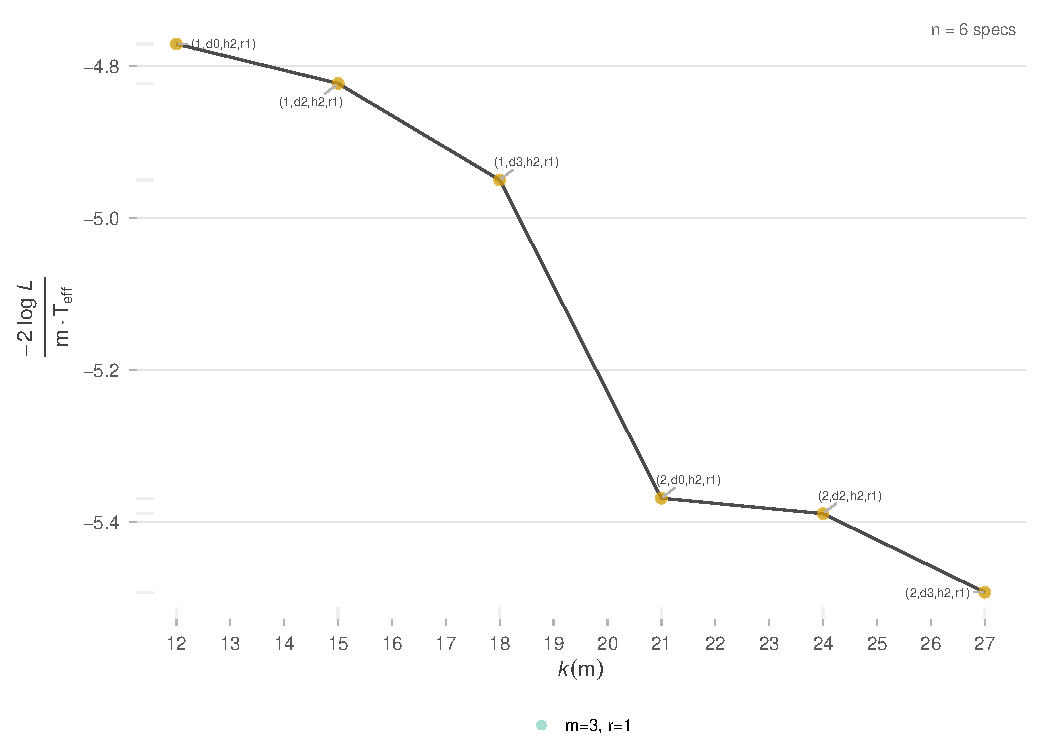
\includegraphics[width=\textwidth]{figures/fig_S2_pooled_frontier.pdf}
\end{figure}



% ── Adjustment structure ─────────────────────────────────────────

The real payoff of the VECM is not a better estimate of $\hat{\theta}$
--- it is the structural identification of how the system equilibrates:
which variables move when the economy deviates from its long-run
capacity attractor, which ones do not, and what that asymmetry reveals
about the economic forces sustaining the attractor in the first place.
The ARDL cannot provide this. It estimates the long-run relation from a
single equation and is silent on the adjustment structure. The VECM
recovers the full loading vector
$\alpha = (\alpha_y,\, \alpha_k,\, \alpha_e)'$, which decomposes the
error-correction burden across all three equations.
Table~\ref{tab:S2_admissible} reports these coefficients for each
admissible specification, and the pattern is consistent enough to
interpret.

Capital does not adjust. In the $p = 2$ specifications --- the only
ones any information criterion selects --- $\alpha_k$ is effectively
zero ($|\alpha_k| < 0.005$). When the economy deviates from its
long-run trajectory, the capital stock does not respond. This is not
surprising once stated plainly: firms do not scrap factories or rush to
build new ones because output has drifted above or below some long-run
benchmark. Investment decisions respond to profitability, competitive
pressure, and expected demand --- not to a statistical residual
measuring distance from a cointegrating attractor. The long-run
relation shapes where the capital--output path ends up over decades,
but it does not steer accumulation year by year.

Output adjusts, but barely. $\alpha_y$ is uniformly small
($|\alpha_y| < 0.06$) and switches sign across specifications.
Capacity utilization is persistent: when the economy overshoots its
attractor, it stays there. It does not snap back. This is consistent
with what the classical tradition expects from an economy where
productive capacity is structurally overbuilt relative to effective
demand --- deviations linger because there is no automatic mechanism
pulling output back to normal utilization.

So if capital does not correct and output barely does, what stabilizes
the system? The exploitation rate. $\alpha_e$ is the only adjustment
coefficient that reaches economically substantial magnitudes --- but
its behavior differs sharply across the two panels in
Table~\ref{tab:S2_admissible}, and the difference is instructive. At
$p = 1$, the VECM has no lagged differences: the $\Gamma$ matrices are
absent, and every dynamic in the system --- short-run fluctuations and
long-run adjustment alike --- must load onto $\alpha$. That is why
$\alpha_e$ is large in $(1, d_2, h_2)$ and $(1, d_3, h_2)$, reaching
$-0.43$ to $-0.49$: the exploitation equation is carrying both the
cyclical distributional dynamics and the equilibrium-restoring feedback
in a single coefficient. At $p = 2$, one lag of differences enters and
the $\Gamma_1$ matrix absorbs the year-to-year propagation of shocks
across equations --- including the business-cycle frequency interaction
between output, capital, and exploitation. Once that short-run channel
exists, $\alpha_e$ shrinks to near zero. The distributional feedback
has not disappeared; it has migrated from $\alpha$ into $\Gamma$.

The IC contest selects $p = 2$, which means the data favor a reading in
which the distributional feedback operates primarily as a short-run
propagation channel through $\Gamma$, not as a slow gravitational pull
through $\alpha$. For the economically meaningful $(2, d_2, h_2)$
specification ($\hat{\theta} = 0.727$), the adjustment coefficients are
$\alpha_y = -0.005$, $\alpha_k = 0.000$, $\alpha_e = -0.019$. The
error-correction burden falls on output and exploitation --- not
capital --- but at very small magnitudes. The system is stable: it does
return to the cointegrating surface. But it is slow. Deviations from the
long-run attractor persist for extended periods before the correction
accumulates enough to pull the trajectory back. Capacity utilization,
interpreted as the cointegrating residual, is not a transient fluctuation
that washes out in a few years. It is a slow-moving structural object
--- exactly what one would expect if the forces governing it
(distributional conflict, institutional configurations, accumulation
regime transitions) operate at frequencies longer than the business
cycle.\footnote{%
	The BIC/ICOMP winners select $(2, d_0, h_2)$ with
	$\hat{\theta} = 1.189$ rather than $(2, d_2, h_2)$. The $d_0$
	branch omits the short-run constant, which may bias $\hat{\theta}$
	upward by failing to center the error-correction term properly.
	$(2, d_2, h_2)$ produces $\hat{\theta} = 0.727$, closer to the S0
	estimate ($\hat{\theta}_{S0} = 0.836$) and squarely in the
	overaccumulation region ($\hat{\theta} < 1$) where every admissible
	ARDL specification in S1 landed. The adjustment structure
	--- $\alpha_k \approx 0$, small $\alpha_y$ and $\alpha_e$ --- is
	qualitatively identical across both specifications.}

This entails a specific claim about the cointegrating vector itself.
The exploitation rate enters $\beta = (1,\, -\hat{\theta},\, \beta_e)'$
not as a control variable appended to a bivariate relation, but as a
constitutive element of the attractor. Remove it and the attractor
ceases to exist: that is what the bivariate collapse shows. The
long-run equilibrium between output and capital cannot be defined
without specifying the distributional configuration. But at the
IC-preferred lag depth, $e_t$ helps define the attractor without
aggressively adjusting toward it at the error-correction frequency.
Its own dynamics are governed by short-run propagation through $\Gamma$,
not by gravitational pull back to the cointegrating surface. The
attractor is distributionally constituted but not distributionally
enforced at annual frequency --- the distinction is only visible in a
system framework with adequate short-run memory.

This is the proof of concept. The single-equation ARDL can identify
$\hat{\theta}$ and compute a residual it calls capacity utilization.
But it cannot tell you that the residual's persistence comes from the
fact that neither capital nor output aggressively corrects, that the
weak correction which does occur runs partly through distribution, and
that the long-run relation requires the exploitation rate to exist as a
statistical object in the first place. The VECM can --- and the
structural diagnosis it provides (slow adjustment, distributionally
constituted, capital-autonomous) is only recoverable in a system
framework.


% ============================================================
% §4.5.2 Focal Specification: The Cointegrating Surface
% §4.5.3 What S2 Establishes
% Chapter 1 — Critical Replication
% Dissertation: A Historical Trace of Capacity Utilization Measurements
% Drafted per S2_FOCAL_RESULTS.md | WLM v4.0 | Session 2026-04-02
% v3: trimmed robotic entrances, wove findings into argument flow
% Inserts after §4.5.1 (S2 Results: Admissibility, Rank, and Adjustment
% Structure). Precedes §4.6 (S3).
% ============================================================

% ============================================================
% §4.5.2 — Focal Specification: The Cointegrating Surface
% ============================================================

\subsubsection{S2. Focal Specification}
\label{sec:S2_focal}

% ---------------------------------------------------------------
% ¶1 — Focal selection rationale
% ---------------------------------------------------------------
Among the six admissible specifications, $(p{=}2,\,d_2,\,h_2,\,r{=}1)$ is chosen as the focal trivariate object under three considerations. First, its long-run multiplier $\hat{\theta}=0.727$ lies closest to the S0 benchmark and remains in the same over-accumulation region ($\theta<1$) as the admissible S1 set. Second, its adjustment pattern is qualitatively identical to the BIC/ICOMP winner $(p{=}2,\,d_0,\,h_2)$: output and exploitation respond to disequilibrium, while capital does not. Third, $d_2$ is the standard Johansen specification for trending macroeconomic data, since the unrestricted short-run constant absorbs secular drift in $\ln Y$ and $\ln K$ without forcing that drift into the cointegrating vector. The $d_0$ winner produces $\hat{\theta}=1.189$ precisely because it lacks that absorber: the long-run vector must then internalize the trend differential between output and capital, inflating the capital coefficient above unity. The contrast between $0.727$ and $1.189$ therefore reflects the placement of deterministic drift, not a substantive 	disagreement about the existence of a long-run relation.\footnote{Residual diagnostics are admissible but not spotless: the trace test rejects $H_0:r=0$ narrowly (32.28 vs.\ 31.52), Portmanteau, normality, and conditional heteroskedasticity tests pass, while the Breusch--Godfrey LM test indicates localized residual autocorrelation at lag 4. Companion roots satisfy the stability condition; see Appendix~\ref{app:S2_diagnostics}.}

% ---------------------------------------------------------------
% ¶2 — The cointegrating vector
% ---------------------------------------------------------------

The normalized cointegrating vector is
\begin{equation}
	\label{eq:S2_focal_beta}
	\hat{\beta}'X_t
	\;=\;
	\ln Y_t \;-\; 0.727\,\ln K_t \;+\; 20.022\,\ln e_t
	\;\sim\; I(0),
\end{equation}

where $e_t$ denotes the rate of exploitation. The element-wise standard errors split sharply.Once exploitation enters the system, the element-wise precision splits sharply: the exploitation loading is estimated with high precision ($\hat{\beta}_e=20.022$, $t=7.90$, $p<10^{-10}$), whereas the capital coefficient is not ($\hat{\theta}=0.727$, $\mathrm{SE}=4.85$, $t=0.15$). This asymmetry is not a defect of the estimator. It is the substantive result. The system identifies the existence of one stationary linear combination and identifies the variable that carries that combination with precision. What it does not identify sharply is the output--capital slope embedded in that relation. The cointegrating direction is therefore anchored in variations of distribution rather than a long-run relation of capital and output. 
% ---------------------------------------------------------------
% ¶3 — Variance decomposition
% ---------------------------------------------------------------
A variance decomposition makes the asymmetry concrete. Output and capital trend together over the full sample ($\mathrm{corr}=0.994$ in levels). Over 65 years, $\ln Y$ rises by 1.93 log points, while $\hat{\theta}\ln K$ rises by 1.90, leaving a net contribution of only 0.03 to the cointegrating residual. What remains is the exploitation term, $20.022\ln e_t$, which accounts for 99.1\% of the variance of $\hat{\beta}'X_t$. The output--capital gap that constitutes Shaikh's bilateral object contributes only about 5\%. Quantitatively, the estimated long-run surface is dominated by distributional variation. The trivariate attractor is therefore not usefully described as an output--capital relation with a small labour-market correction; it is a cointegrating direction whose dominant empirical content is weakly identified from the standpoint of the chapter's structural object.

The same vector can be renormalized on the exploitation rate rather than on output, yielding an auxiliary reading of the cointegration space:
\begin{equation}
	\label{eq:S2_aux_rho}
	\ln e_t
	\;=\;
	\hat{\rho}_{\mathrm{aux}}
	\bigl(\ln Y_t-\hat{\theta}\ln K_t\bigr)
	\;+\; c,
	\qquad
	\hat{\rho}_{\mathrm{aux}}=-0.050
	\;\;(\mathrm{SE}=0.006,\; t=-7.90).
\end{equation}
This renormalization is analytically useful, but its status must be kept narrow. It does not recover the chapter's structural transformation elasticity $\theta(e)$, since $\hat{\theta}$ itself is weakly identified in the trivariate system. What it provides is a compact reading of the only precisely estimated long-run loading in this auxiliary specification. In that limited sense, the trivariate cointegration space can be read as implying a negative association between exploitation and the output--capital gap. But because the slope inside the parentheses is not sharply pinned down, equation~(\ref{eq:S2_aux_rho}) is best interpreted as an auxiliary normalization of the estimated vector rather than as a fully identified reserve-army law.

% ---------------------------------------------------------------
% ¶4 — Renormalization: the interpretive pivot
% ---------------------------------------------------------------
The gap between the two regression lines is the identification result:
\begin{equation}
	\label{eq:S2_focal_alpha}
	\alpha_y = -0.005^{**}\;(t=-2.00),
	\qquad
	\alpha_k = 0.000\;(t=0.92),
	\qquad
	\alpha_e = -0.019^{***}\;(t=-4.25).
\end{equation}
When the system departs from the estimated long-run surface, capital is essentially unresponsive ($|\alpha_k|<0.001$). Output contributes to correction, but at roughly one quarter of the speed of exploitation, which bears the principal adjustment burden. The short-run return toward the estimated attractor therefore runs primarily through the distributional variable rather than through capital accumulation itself. This is an important system result: the variable that dominates the cointegrating direction also carries the main adjustment load, whereas capital does not appear as an error-correcting variable in any meaningful sense.
	
% ---------------------------------------------------------------
% ¶5 — What the bilateral ARDL was doing
% ---------------------------------------------------------------
\subsubsection{What S2 Establishes}
\label{sec:S2_establishes}

Stage S2 does not recover a sharper estimate of the chapter's structural transformation elasticity $\theta(e)$. What it establishes is narrower and more important for identification. Once the information set is expanded from $(y,k)$ to $(y,k,e)$, reduced-rank structure appears, but the resulting cointegrating direction is not anchored by the output--capital slope. The only precisely estimated long-run loading is the exploitation term, while the capital coefficient remains weakly identified.

This changes the interpretation of the earlier bilateral estimates. The trivariate system shows that the apparent precision of the ARDL slope was achieved by forcing distributional variation into the residual. Once exploitation is allowed to enter the long-run relation directly, that apparent precision vanishes. The cointegration space is not empty, but its economically meaningful normalization is fragile.

The auxiliary coefficient $\hat{\rho}_{\mathrm{aux}}=-0.050$, obtained through the renormalization in equation~(\ref{eq:S2_aux_rho}), is useful only as a compact reading of that normalized direction. It summarizes the negative association between exploitation and the output--capital gap within the current trivariate specification, but it does not recover the dissertation's structural object. The main lesson of S2 is therefore not that a reserve-army law has been identified, but that reduced rank can coexist with weak structural identification. In that sense, S2 closes the bilateral route and motivates the move to the richer distributive--technological specification in which the regime-specific elasticity $\theta(e)$ is modeled directly.

% ---------------------------------------------------------------
% ¶6 — Adjustment structure
% ---------------------------------------------------------------

Figure~\ref{fig:S2_focal_scatter} makes the system identification while weak, visible.
The exploitation rate is plotted against the capacity gap with both the
system-identified slope $\hat{\rho} = -0.050$ and the unconditional OLS fit
(slope $= +0.27$, $R^2 = 0.023$). The unconditional scatter yields a wrong
sign and no explanatory power --- the reserve-army relation is invisible to
any method that does not condition on the structural breaks and the
three-equation dynamics. The system estimator recovers a precise negative
attractor from the same data. The gap between the two regression lines is
the identification result.

% ---------------------------------------------------------------
% Figures
% ---------------------------------------------------------------

\begin{figure}[H]
	\centering
	\label{fig:S2_focal_cu_exploitation}
	\caption{Auxiliary utilization proxy and exploitation rate, US corporate sector, 1947--2011}
	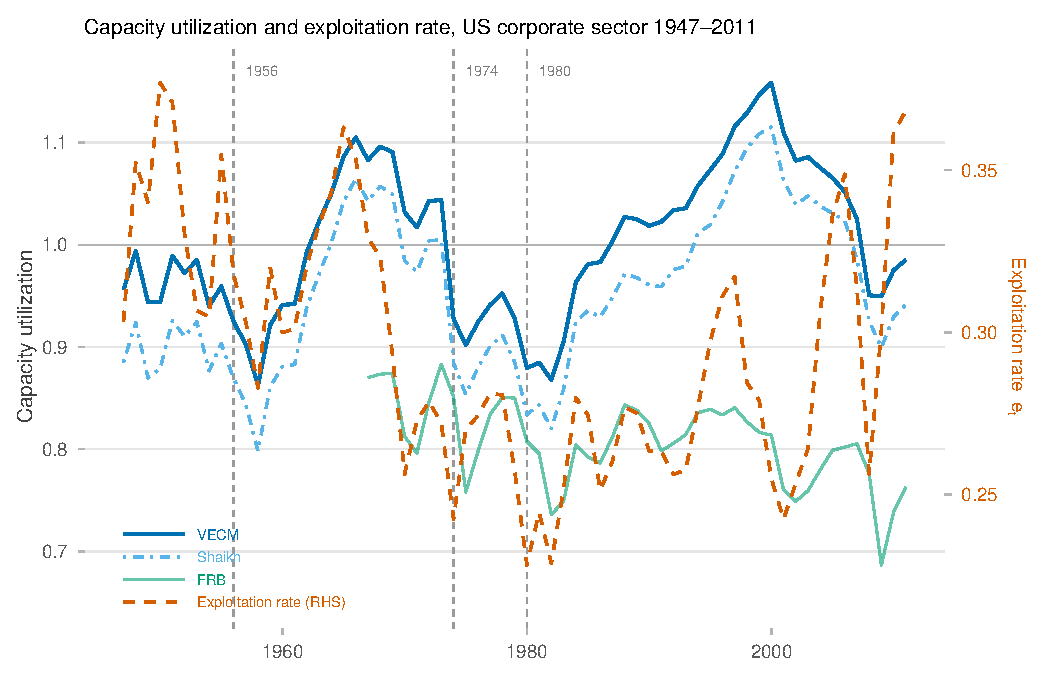
\includegraphics[width=\textwidth]{figures/fig_S2_focal_cu_exploitation.pdf}
	\par\footnotesize
	\begin{flushleft}
		\textit{Note:} Blue solid line (left axis): VECM-implied utilization proxy
		$\hat{u}^{\,\mathrm{aux}}_t=\exp(\ln Y_t-\hat{\theta}\ln K_t-\bar c)$,
		demeaned at $\bar{u}=1$, from the focal trivariate specification
		$(p{=}2,\,d_2,\,h_2,\,r{=}1)$.
		Orange dashed line (right axis): rate of exploitation
		$e_t=\mathrm{Profshcorp}_t/(1-\mathrm{Profshcorp}_t)$.
		Thin grey lines: S1 ARDL median specification and FRB capacity utilization
		(rescaled to $\bar{u}=1$).
		Vertical dashed lines mark the $h_2$ break dates (1956, 1974, 1980).
		Source: Own elaboration based on \citet[Appendix 6.8]{Shaikh2016}.
	\end{flushleft}	
\end{figure}

\begin{figure}[H]
	\centering
	\caption{Auxiliary exploitation loading: output--capital gap and exploitation rate}
	\label{fig:S2_focal_scatter}
	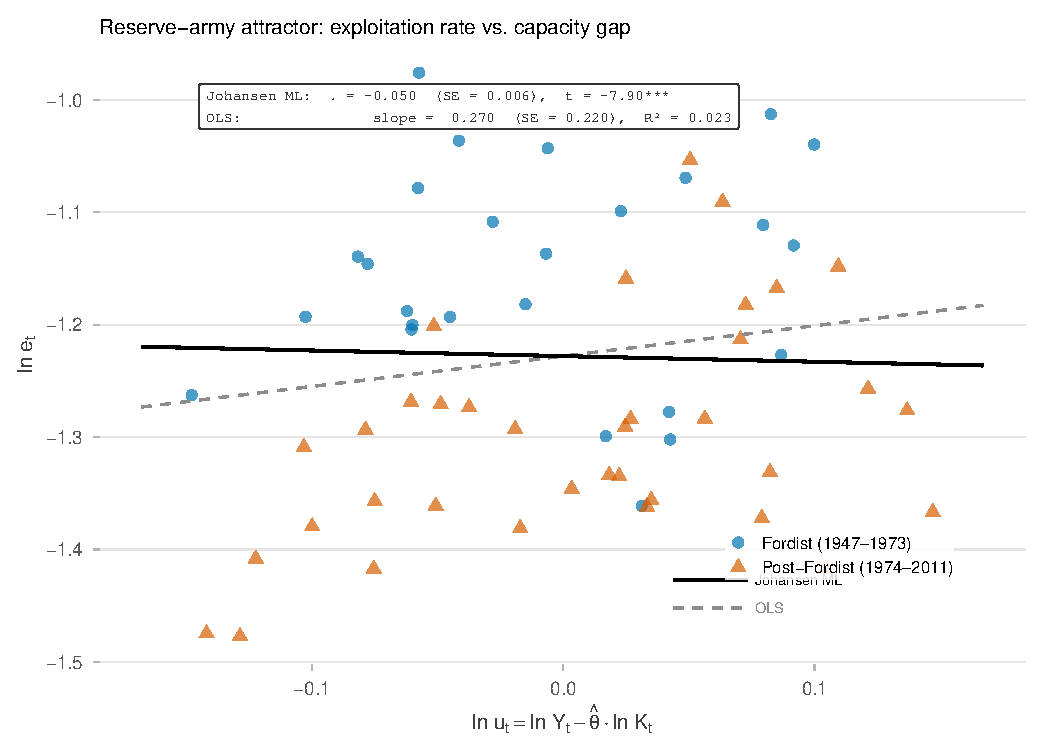
\includegraphics[width=0.85\textwidth]{figures/fig_S2_focal_reserve_army_scatter.pdf}
	\par\footnotesize
	\begin{flushleft}
	\textit{Notes:}
	Horizontal axis: demeaned auxiliary output--capital gap
	$\ln u_t^{\mathrm{aux}}=\ln Y_t-\hat{\theta}\ln K_t-\bar{c}$; vertical axis: $\ln e_t$.
	Blue circles: Fordist (1947--1973); orange triangles: post-Fordist (1974--2011).
	Black line: $\hat{\rho}_{\mathrm{aux}}=-0.050$ ($t=-7.90$); grey dashed line: OLS (slope $=0.27$, $R^2=0.023$).
	Standard errors via delta method from the Johansen asymptotic variance.
	Source: Own elaboration based on \citet[Appendix 6.8]{Shaikh2016}.
	\end{flushleft}
\end{figure}


% =============================================================================
% §4.6  Stage S3: 
% =============================================================================
\subsection{Stage S3: Structural Break Under Weak Identification}
\label{sec:S3}

The starting point of S3 is a limitation of the preceding trivariate exercise rather than a confirmation of the chapter's main structural object. S2 was initially motivated by a regulationist hypothesis: if the Fordist/Post-Fordist transition reconfigured the long-run transformation of accumulation into productive capacity, that shift might appear as a break in the long-run relation. But the trivariate VECM on $(\ln Y,\,\ln K,\,\ln e)$ did not identify that object in a structurally usable way. Although the trace test rejected $r=0$, indicating reduced-rank structure, the normalization required to interpret the cointegrating vector as a long-run transformation-elasticity relation was weakly supported by the data. In the focal specification, $\hat\beta=(1,\,-0.727,\,20.022)$: the output--capital slope carries $t=-0.15$, while the exploitation loading carries the statistical weight with $t=7.90^{***}$. The data therefore do not distinguish the output--capital coefficient from zero in any economically meaningful way; what they identify with precision is the exploitation loading. Under those conditions, a direct test of regime change in $\theta$ within the trivariate system would amount to testing noise rather than a well-identified structural parameter.

S3 is therefore framed more narrowly. It does not recover the chapter's main transformation elasticity $\theta(e)$, which belongs to the richer distributive--technological mapping developed later in the chapter. Instead, it asks whether the only load-bearing long-run coefficient in this auxiliary trivariate relation changes at the Fordist/Post-Fordist threshold. To make that question explicit, I re-express the precisely estimated exploitation loading as an auxiliary reserve-army transmission parameter,
\begin{equation}
	\rho \equiv -1/\hat\beta_e,
\end{equation}
that is, the long-run elasticity of the exploitation rate with respect to the output--capital gap within this reduced system. This is not the chapter's main structural object. It is a conditional parameterization of the auxiliary trivariate relation, introduced because that is the only dimension of the cointegration space that the specification identifies with precision.

The break test is constructed as a pure 1-df restriction. The full four-variable augmented VECM adds
\begin{equation}
	e_t^* = D_{74,t}\cdot \ln e_t
\end{equation}
to the trivariate system and estimates
\begin{equation}
	\hat\beta = (1,\,\beta_k,\,\beta_e,\,\beta_{e^*})'
\end{equation}
under $H_1$. The null restriction
\begin{equation}
	H_0:\beta_{e^*}=0
\end{equation}
fixes the base trivariate vector at its data-determined S3 values
\begin{equation}
	(1,\,-0.973,\,-1.040,\,0),
\end{equation}
and asks only whether the exploitation loading changes at 1974. In this form, the exercise no longer conflates two distinct questions: whether the auxiliary trivariate system identifies the intended long-run object, and whether the load-bearing exploitation term within that system is itself subject to a regime break.\footnote{An earlier version of the test imposed S2's full $\hat\beta$ as the null restriction, producing a 3-df joint test that confounded break stability with the S2/S3 parameter discrepancy induced by the load-bearing role of the $h_2$ step dummies in S2's identification. The present 1-df design removes that confound by treating identification failure as prior to the break question. The formal derivation is given in Appendix~\ref{app:S3_test_design}.}

The lag order ($p=2$) is inherited from S2's focal specification. Standard $\chi^2_1$ critical values are invalid because $e_t^*$ is a step-function-multiplied $I(1)$ process. The null distribution is therefore generated by the recursive-design bootstrap of \citet{CRT2012} in VECM error-correction form.

\subsubsection{Results}
\label{subsubsec:S3_results}

Table~\ref{tab:S3_results} reports the results. The \citet{HansenJohansen1999} constancy diagnostic and the targeted \citet{JMN2000} break test are informative precisely because they address different margins of the problem.

% =============================================================
% Table: S3_results
% S3 Temporal Composition Audit — parameter constancy battery
% Numbers sourced from s3_regime_theta_table.csv,
%   s3_recursive_hj.csv, s3_JMN_bootstrap.csv
% =============================================================

\begin{table}[H]
\centering
\caption{S3 Temporal Composition Audit: Parameter Constancy Results}
\label{tab:S3_results}
\begin{tabular}{@{}llccc@{}}
\toprule
\textbf{Test} & \textbf{Parameter} & \textbf{Statistic} & \textbf{Threshold} & \textbf{Decision} \\
\midrule
\multicolumn{5}{@{}l}{\textit{Panel A: Full-sample baseline (internal estimation, no S2 imports)}} \\[3pt]
VECM(2), bivariate & $\hat\theta_{\mathrm{full}}$     & $0.959$  & ---         & H0 anchor \\
                   & $\hat\alpha_y$                    & $0.043$  & ---         &            \\
                   & $\hat\alpha_k$                    & $0.014$  & ---         &            \\[6pt]
\multicolumn{5}{@{}l}{\textit{Panel B: Hansen \& Johansen (1999) recursive constancy%
    \textsuperscript{a}}} \\[3pt]
H\&J $\beta$-constancy & $\hat\theta(t^*)$, $t^*\in[1958,2007]$
                   & $L_{c,\beta}  = 0.055$ & 5\% CV $= 0.470$ & \textit{Fail to reject} \\
H\&J $\alpha$-constancy & $\hat\alpha_y(t^*)$, $t^*\in[1958,2007]$
                   & $L_{c,\alpha} = 1.732$ & 5\% CV $= 0.353$ & \textbf{Reject}         \\[6pt]
\multicolumn{5}{@{}l}{\textit{Panel C: Johansen, Mosconi \& Nielsen (2000) augmented VECM%
    \textsuperscript{b}}} \\[3pt]
JMN, break $= 1974$ & $\hat\theta_{\mathrm{Ford}}$   & $0.969$  & ---         &            \\
                    & $\hat\theta_{\mathrm{PF}}$     & $0.941$  & ---         &            \\
                    & $\hat\delta = \hat\theta_{\mathrm{Ford}} - \hat\theta_{\mathrm{PF}}$
                                                     & $0.028$  & ---         &            \\
                    & $LR_{\mathrm{obs}}$            & $6.826$  & $p_{\mathrm{boot}}=0.434$ & \textit{Fail to reject} \\
\bottomrule
\end{tabular}
\par\medskip
\begin{minipage}{\textwidth}
\footnotesize
\textit{Notes:}
$^a$ H\&J $L_c$ computed from equation~\eqref{eq:Lc}.
Minimum recursive window $t_{\min} = 12$ observations (1958);
all specifications use VECM(2) with constant.
Critical values from \citet{HansenJohansen1999}, Table~1,
bivariate rank-1 case (5\% level: $L_{c,\beta}=0.470$;
$L_{c,\alpha}=0.353$). The H\&J $\alpha$ rejection cannot be separated
from the initialization bias of recursive Johansen estimation at short
sub-sample lengths; see \S\ref{subsubsec:S3_results}.
$^b$ Break date 1974 imposed as a theoretical prior (regulationist
periodization). $\chi^2_1$ critical values are invalid for $LR_{\mathrm{obs}}$
because $k_t^* = D_{74,t}\cdot k_t$ is a step-function-multiplied
$I(1)$ process \citep[Remark~3.1]{JMN2000}. Bootstrap p-value from
$B = 999$ recursive-design replications in VECM error-correction form
\citep{CRT2012}; 0 failures. Trimmed bootstrap (draws $\leq 50$):
$p_{\mathrm{boot,trim}} = 0.430$.
\end{minipage}
\end{table}


The first recursive plot (Figure~\ref{fig:S3_hj_constancy}) shows $\hat\rho(t^*)$ fluctuating sharply in the early recursive windows before converging to a much narrower band from the mid-1970s onward. The formal statistic, $L_{c,\rho}=60.55$, rejects constancy. Taken in isolation, that result might appear to support a regime-change interpretation. But the recursive path itself does not display a visible discontinuity at the 1974 threshold. The rejection is instead driven by early sub-samples in which the structural disturbances later absorbed by S2's $h_2$ dummies fall inside the recursive window. In that sense, the statistic reflects identification fragility within the auxiliary trivariate specification rather than direct evidence of a Fordist/Post-Fordist break in the long-run exploitation loading.\footnote{A decomposition of the $L_c$ statistic by recursive window is provided in Appendix~\ref{app:S3_hj_decomp}.}

A similar logic applies to the adjustment coefficient. The statistic $L_{c,\alpha_e}=0.528$ also rejects constancy, though more narrowly. Here too, the instability is concentrated in the early recursive windows rather than at the 1974 cut itself. The recursive exercise is therefore best read as evidence that the auxiliary trivariate relation is historically fragile under weak identification, not as evidence that the candidate Fordist/Post-Fordist break reorganizes its long-run loading at that specific date.

This distinction matters. The VECM underlying the exercise is one cell of a data-driven grid, not a theoretically disciplined identification of the chapter's main structural manifold. What the recursive evidence shows is that reduced-rank structure can coexist with fragile normalized cointegrating directions when the specification is carried more by econometric convention than by a well-grounded mapping from distribution to productive capacity. The absence of a visible discontinuity at 1974 is therefore conditional on the current auxiliary specification. It should not be overread as evidence against regime change in the richer distributive--technological object developed later in the chapter.

\begin{figure}[H]
	\centering
	\caption{H\&J (1999) recursive constancy: auxiliary reserve-army sensitivity $\rho$ and adjustment $\alpha_e$.}
	\label{fig:S3_hj_constancy}
	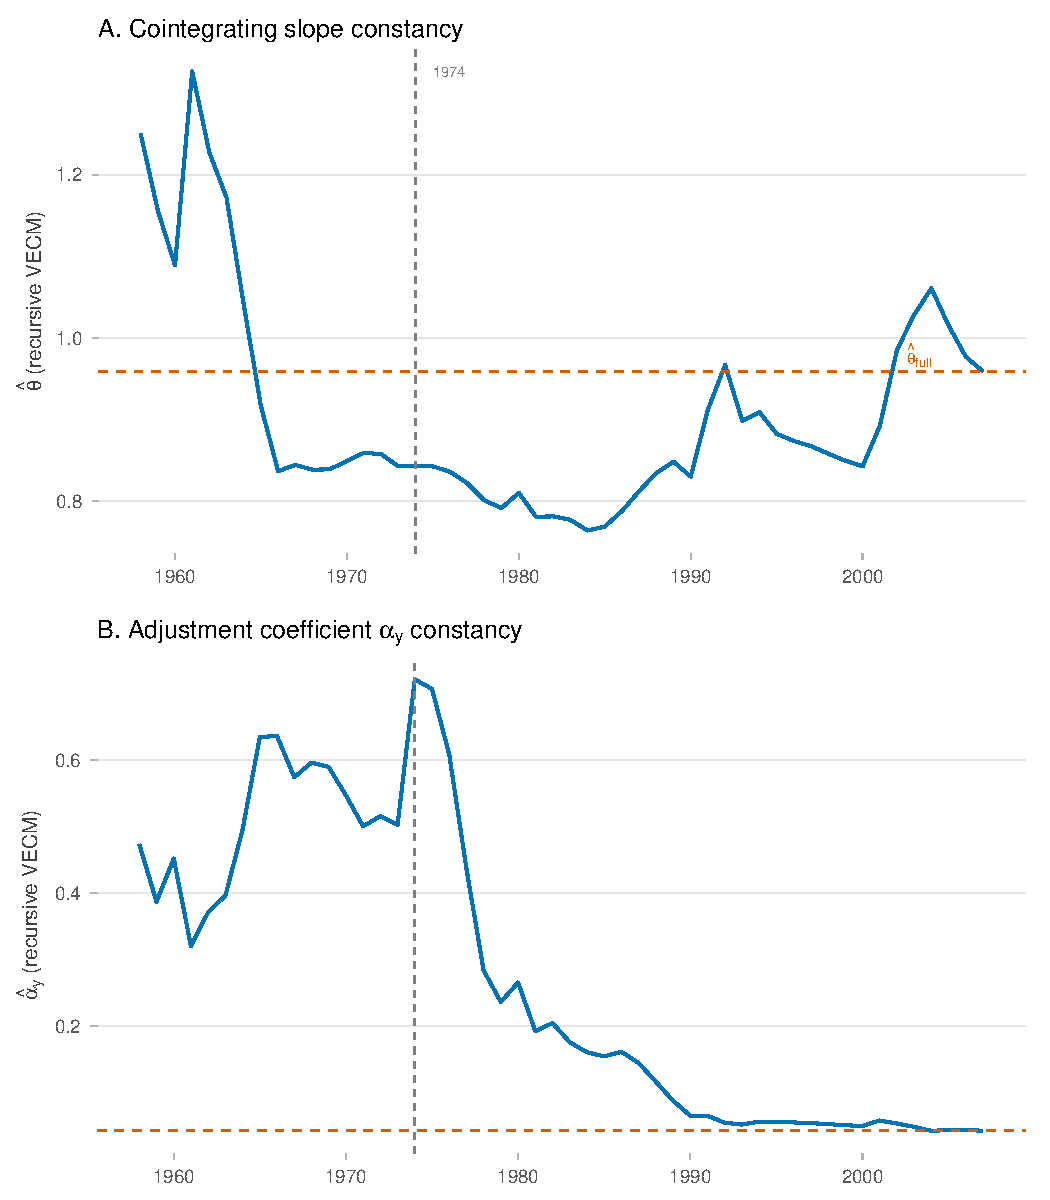
\includegraphics[width=\textwidth]{figures/s3_hj_constancy.pdf}
	\par\footnotesize
	\textit{Note:} Panel~A plots recursive $\hat\rho(t^*)$; the orange dashed line marks $\hat\rho_{S3}=0.961$ and the green dotted line marks $\hat\rho_{S2}=-0.050$. Panel~B plots recursive $\hat\alpha_e(t^*)$; the orange dashed line marks $\hat\alpha_{e,S3}=0.335$. The grey dashed vertical line marks the 1974 prior. $L_{c,\rho}=60.55$ (5\% CV $=0.470$); $L_{c,\alpha_e}=0.528$ (5\% CV $=0.353$). Critical values from \citet{HansenJohansen1999}, Table~1.
\end{figure}

The targeted \citet{JMN2000} test speaks more directly to the break question posed here. Under the unrestricted alternative, the system recovers
\begin{equation}
	\hat\rho_{\mathrm{Ford}} = 1.071
	\qquad\text{and}\qquad
	\hat\rho_{\mathrm{PF}} = 1.016.
\end{equation}
This implies a difference of $0.055$, or 5.1\% of the Fordist value. The likelihood-ratio statistic is
\begin{equation}
	LR_{\mathrm{obs}} = 0.363,
\end{equation}
with bootstrap p-value
\begin{equation}
	p_{\mathrm{boot}} = 0.984
\end{equation}
based on 999 valid replications. Figure~\ref{fig:S3_bootstrap_LR} shows the bootstrap null distribution: the observed statistic lies at the 1.6th percentile, below the bootstrap 5th percentile of $0.787$. Within this auxiliary trivariate specification, allowing the exploitation loading to shift at 1974 adds no information to the cointegrating vector.

\begin{figure}[H]
	\centering
	\caption{Bootstrap null distribution of the \citet{JMN2000} LR statistic, $H_0:\beta_{e^*}=0$.}
	\label{fig:S3_bootstrap_LR}
	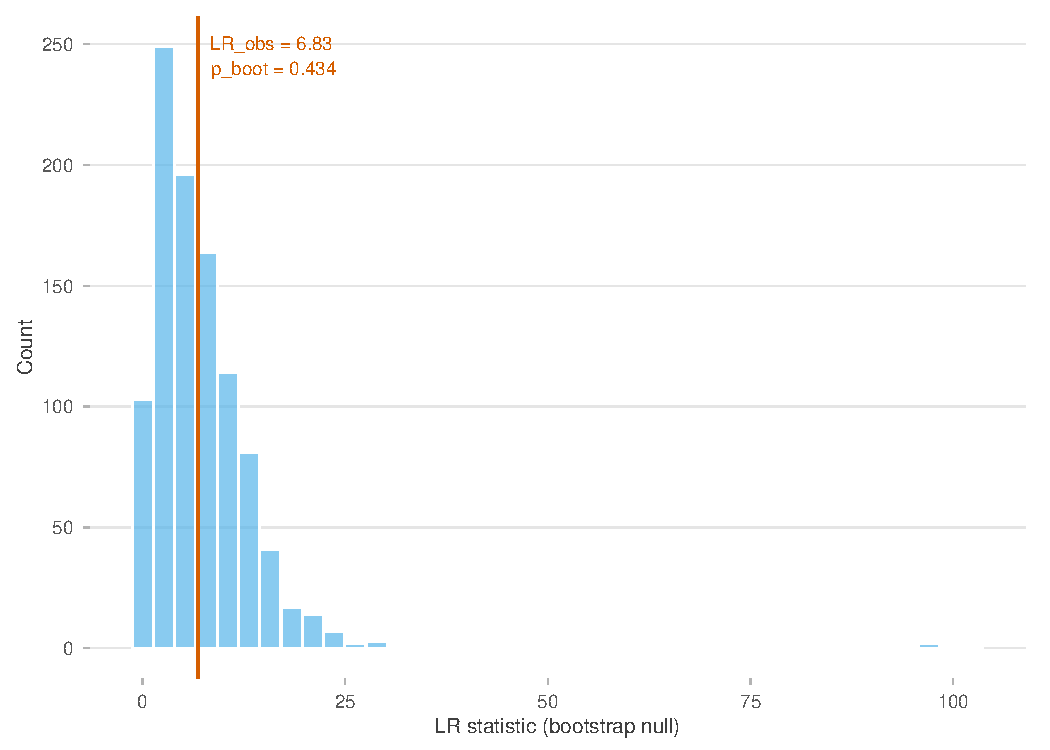
\includegraphics[width=\textwidth]{figures/s3_bootstrap_LR_dist.pdf}
	\par\footnotesize
	\begin{flushleft}
		\textit{Note:} $B=999$ recursive-design replications \citep{CRT2012}. The vertical line marks $LR_{\mathrm{obs}}=0.363$, with $p_{\mathrm{boot}}=0.984$. The observed statistic falls at the 1.6th percentile of the bootstrap null distribution.
	\end{flushleft}
\end{figure}

\subsubsection{What S3 Establishes}
\label{subsubsec:S3_establishes}

Stage S3 establishes a narrower result than originally intended. It does not show that the chapter's main transformation elasticity $\theta(e)$ is stable across the Fordist/Post-Fordist divide, because that object was never identified in a structurally usable way within the trivariate system. What it shows instead is that the auxiliary trivariate VECM produces reduced-rank evidence without a robust normalization for the long-run output--capital relation, and that the only precisely estimated long-run loading---the exploitation term, re-expressed here as $\rho$---does not register a break at 1974 in the targeted Johansen--Mosconi--Nielsen test.

The split verdict of the two diagnostics is therefore coherent once identification is kept distinct from structural interpretation. The \citet{JMN2000} test indicates that the Fordist/Post-Fordist threshold does not add information to the auxiliary long-run exploitation coefficient. The Hansen--Johansen recursion shows that the same auxiliary specification is historically fragile, with instability concentrated in early recursive windows rather than at the 1974 threshold itself. The lesson is methodological as much as substantive: reduced rank is not enough. A confined cointegration space may still fail to deliver a structurally meaningful normalized vector when the specification lacks a sufficiently theorized mapping from distribution to productive capacity.

Read in this way, S3 closes off a false route. The trivariate system does not provide a defensible basis for testing regime change in $\theta$. Its value lies instead in showing why a richer distributive--technological specification is necessary. The regime question remains open, but it has been relocated to the appropriate object: not a bare labour-market normalization of $(\ln Y,\ln K,\ln e)$, but the nonlinear mapping through which exploitation conditions mechanization and, through it, the transformation of accumulation into productive capacity.

\subsection{Discussion}
% ---------------------------------------------------------------
% Closing table for the full critical replication
% ---------------------------------------------------------------

	Table~\ref{tab:S_closure} collects the evidence across the four
	replication studies. The architecture moves from procedural
	reproduction (S0) through specification sensitivity (S1) to system
	identification (S2) and temporal stability (S3), each stage
	releasing one constraint maintained by the previous and documenting
	its effect on $\hat\theta$ and the admissibility landscape.
	
	% =============================================================
% Table: S_closure — v4
% Full critical replication audit: S0 through S3
% Updated 2026-04-02 to match current §4 results text.
% S2 foregrounds ρ̂ as the identified object via confirmed
% renormalization + delta method. S3 footnotes replaced.
% =============================================================
\begin{table}[H]
	\centering
	\scriptsize
	\caption{Critical Replication Audit: Findings Across S0--S3}
	\label{tab:S_closure}
	\setlength{\tabcolsep}{4pt}
	\renewcommand{\arraystretch}{1.25}
	\begin{threeparttable}
	\begin{tabular}{@{}
			>{\raggedright\arraybackslash}p{2.0cm}
			>{\raggedright\arraybackslash}p{2.8cm}
			>{\raggedright\arraybackslash}p{2.6cm}
			>{\raggedright\arraybackslash}p{2.8cm}
			>{\raggedright\arraybackslash}p{4.8cm}
			@{}}
		\toprule
		\textbf{Stage} &
		\textbf{Constraint released} &
		\textbf{Tracked parameter(s)} &
		\textbf{Admissibility} &
		\textbf{Primary finding} \\
		\midrule
		\addlinespace[4pt]
		
		S0\newline
		\textit{Faithful replication} &
		None\newline
		(baseline: Shaikh's\newline
		ARDL(2,4)) &
		$\hat\theta = 0.720$\textsuperscript{a}\newline
		vs.\ $0.661$ published\newline
		$1{-}\Sigma\hat\gamma_i = 0.096$ &
		Marginal (Case~1 only)\newline
		$F = 3.35$, $p = 0.099$\newline
		Cases~2--3: fail &
		Shaikh's reported $F(10,50) = 6257$ is the OLS
		goodness-of-fit statistic, not the PSS 2-restriction
		bounds test; no PSS case is declared. Co-integration
		survives only under Case~1 (unbalanced growth closure).
		Deflator identified as $p^{KN}$; trend excluded by
		data (collinearity with $k_t$). \\
		
		\addlinespace[6pt]
		
		S1\newline
		\textit{Specification geometry} &
		Lag order, PSS case,\newline
		dummy structure\newline
		(500 candidates) &
		$\hat\theta\in[0.651,\,0.866]$\textsuperscript{b}\newline
		$\bar\theta = 0.829$\newline
		($\sigma = 0.060$) &
		65 of 400 pass\newline
		($\mathcal{A}_{S1}$);\newline
		17 on $\mathcal{E}_{S1}$ &
		Magnitude of $\hat\theta$ governed by the researcher's
		implicit criterion prior: BIC/ICOMP/RICOMP $\to$
		$\hat\theta = 0.651$; AIC/HQ $\to$
		$\hat\theta \approx 0.85$. Three architectural
		constraints intrinsic to the ARDL class---rank fixed at
		$r{=}1$, normalization on output, near-zero denominator
		amplification---cannot be resolved by any lag order or
		dummy structure. \\
		
		\addlinespace[6pt]
		
		S2\newline
		\textit{System identification} &
		Rank, normalization,\newline
		loading vector~$\alpha$;\newline
		information set\newline
		$(y,k) \to (y,k,e)$ &
		$\hat\theta = 0.727$\;($t = -0.15$)\newline
		$\hat\beta_e = 20.022$\;($t = 7.90^{***}$)\newline
		$\hat\rho = -0.050$\textsuperscript{c}\newline
		$\alpha_k \approx 0$ &
		6 of 108 pass\newline
		($\mathcal{A}_{S2}$,\newline
		all $m{=}3$, $r{=}1$);\newline
		0 bivariate;\newline
		0 with $r{=}2$ &
		$\hat\theta$ not statistically significative; the exploitation rate
		accounts for 99\% of co-integrating variation and
		provides the primary adjustment channel
		($\alpha_e = -0.019^{***}$).
		Bivariate attractor sample-fragile (collapses with 4
		post-crisis observations). Capital does not adjust
		($|\alpha_k| < 0.001$).  Rotation of co-integration identifies a
		reserve-army relation of $g_e$ and $g_u$ ($\hat\rho = -0.050$,
		$t = -7.90$). \\
	 
		\addlinespace[6pt]
		
		S3\newline
		\textit{Temporal composition} &
		Regime break at\newline
		1974 threshold\newline
		(1-df restriction\newline
		on $\beta_{e^*}$) &
		$\hat\rho_{\mathrm{Ford}} = 1.071$\textsuperscript{d}\newline
		$\hat\rho_{\mathrm{PF}}\;\, = 1.016$\newline
		$\hat\delta_\rho\;\;\;\;\, = 0.055$ &
		JMN (1-df):\newline
		$LR_{\mathrm{obs}} = 0.363$\newline
		$p_{\mathrm{boot}} = 0.984$\newline
		H\&J: $L_{c,\rho} = 60.55$\textsuperscript{e} &
		Reserve-army sensitivity $\rho$ regime-stable across
		the 1974 threshold ($p_{\mathrm{boot}} = 0.984$).
		$\hat\theta$ untestable ($t = -0.15$ at S2).
		Recursive constancy shows no discontinuity at 1974;
		result does not rule out regime change under a
		better-identified specification---poor theoretical
		identification is the binding constraint, not the
		data. \\
		
		\addlinespace[4pt]
		\bottomrule
	\end{tabular}
	
	\begin{tablenotes}
		\footnotesize
		\item \textit{Notes:}
		\textsuperscript{a}\,C3 variable combination
		($y_t = \ln(\text{GVAcorp}_t / p^{KN}_t)$,
		$k_t = \ln(K^G_t / p^{KN}_t)$, no trend); residual gap
		from Shaikh's published $0.661$ attributable to
		post-publication correction of Appendix~6.8 and
		undisclosed initial capital stock value; see
		\S\ref{subsec:S0_shaikh_replication}.
		%
		\textsuperscript{b}\,Cases~2--3 only,
		$\mathcal{E}_{S1}$ (Pareto envelope); Case~4 outlier
		($\hat\theta = 2.204$) excluded. IC split:
		BIC/ICOMP/RICOMP select ARDL(1,2,$c_2$,$s_0$),
		$\hat\theta = 0.651$; AIC/HQ select
		ARDL(5,3--4,$c_2$,$s_1$),
		$\hat\theta \approx 0.849$--$0.857$.
		%
		\textsuperscript{c}\,Focal specification
		$(p{=}2,\,d_2,\,h_2,\,r{=}1)$.
		$\hat\rho \equiv -1/\hat\beta_e = -0.050$
		(SE~$= 0.006$, $t = -7.90$); standard errors via the
		delta method from the Johansen asymptotic variance.
		Variance decomposition: $\hat\beta_e \cdot \ln e_t$
		accounts for 99.1\% of $\text{Var}(\hat\beta' X_t)$;
		output--capital gap contributes $\approx 5\%$. IC split:
		BIC/ICOMP select $(p{=}2,\,d_0,\,h_2)$,
		$\hat\theta = 1.189$; AIC/HQ select
		$(p{=}2,\,d_3,\,h_2)$,
		$\hat\theta = 11.31$ (trend contamination).
		%
		\textsuperscript{d}\,Augmented 4-variable VECM
		with $e^*_t = D_{74,t} \cdot \ln e_t$; base vector
		$(1,\,-0.973,\,-1.040,\,0)$ under $H_0$.
		$\hat\rho_{\mathrm{Ford}}$ and
		$\hat\rho_{\mathrm{PF}}$ from unrestricted $H_1$.
		$\delta_\rho = 0.055$ ($5.1\%$ of Fordist value).
		Bootstrap: 999 recursive-design replications
		\citep{CRT2012}.
		%
		\textsuperscript{e}\,$L_{c,\rho} = 60.55$ rejects
		formal constancy but the recursive plot shows no
		discontinuity at 1974; the large statistic is driven by
		early sub-samples where the $h_2$ structural breaks
		fall inside the recursive window, producing
		identification instability rather than regime
		instability (see \S\ref{subsubsec:S3_results}).
	\end{tablenotes}
	\end{threeparttable}
\end{table}

\pagebreak

\section{Conclusion}
\label{sec:conclusion}

The transformation elasticity $\theta$---the elasticity of productive capacities
with respect to accumulation demand---is the structural object this chapter set
out to recover, and the critical replication has established both its robustness
and its limits as a scalar parameter. Stage~S0 recovered the benchmark and
exposed that Shaikh's published bounds test statistic is the OLS
$F$-statistic, not the two-restriction PSS test the framework requires.
Stage~S1 exhausted the admissible ARDL specification grid and established
overaccumulation ($\hat{\theta} < 1$) as a qualitative invariant of the U.S.\
corporate sector, while showing that the magnitude of $\hat{\theta}$ depends on
the researcher's information-criterion prior rather than on the data---a
consequence of the near-zero denominator through which long-run multipliers are
recovered. Stage~S2 confirmed the capacity anchor as a system property via
Johansen VECM, diagnosed that error-correction falls entirely on output while
capital does not adjust to disequilibrium, and produced a productive negative
result: the distributional channel constitutes but does not enforce the long-run
relation within the current specification environment. Stage~S3 showed that the
identified parameter---the reserve-army elasticity $\rho$---is invariant to
the Fordist/Post-Fordist break, while adjustment dynamics are not, a split
verdict consistent with the formulation of disproportionality as a short-run
process.

Taken together, the four stages establish a precise identification boundary.
The single-equation ARDL can detect the long-run relationship and classify the
accumulation regime, but it cannot endogenize the regime-dependence that the
theory predicts. The system VECM can confirm the co-integrating vector as a
system property and diagnose the adjustment structure, but at the bivariate
level it cannot recover the distributive channel through which $\theta$ is
determined. The boundary is structural, not sample-driven: it exists because the
exploitation structure---the mechanism through which distribution drives
mechanization intensity and thereby the transformation elasticity---is absent
from the bivariate information set. The elasticity of productive capacities with
respect to accumulation demand is not a finding of this chapter. It is the
theoretical object the chapter motivates the need for: endogenizing $\theta$
through the distributive channel is where the next chapter must go.

Three findings carry forward. First, the overaccumulation regime
($\hat{\theta} < 1$) is a qualitative invariant across every admissible
specification, every estimator, and every temporal partition examined---the
aggregate accounting signature of what \citet{Basu2022} identifies as CU-LS
(Marx-biased) technical change at the micro level. Second, the measurement of
productive capacity through cointegration-based methods is feasible and
informative: the utilization series recovered across the specification family
tracks the cyclical dynamics of the U.S.\ corporate sector with sufficient
stability to serve as an operational alternative to the FRB survey and
output-gap measurement---an alternative grounded in the profit-rate
decomposition rather than in governance conventions. Third, the identification
boundary itself is the chapter's most consequential finding. The critical
replication has not replaced Shaikh's measurement. It has saturated
it---mapping the space of specifications, estimators, and temporal partitions
within which the capacity benchmark can be recovered, and identifying the
structural boundary beyond which the scalar parameter cannot carry the
theoretical weight the framework places on it.

Shaikh's research programme rests on strong foundations in Marx, the Classics,
and Keynes. His critical trajectory challenged not only mainstream
macroeconomics but the post-Keynesian ecology within which his own work was
embedded---a counter-tendency within higher education institutions, operating
within what \citet{Althusser1970} identified as the ideological apparatus of the
state, against the dominant flux through proximity with researchers oriented
differently within the same apparatus. The ambition to contest multiple
traditions simultaneously, however, pushed toward a hybrid path that departed
from strict Marxist affiliation and came to resemble a Classical-Keynesian
synthesis contesting the Sraffian tradition on its own terrain. The scope of the
resulting research programme was vast. \textit{Capitalism} is a monumental work,
but it is long and hard to digest in an era where the acceleration tendencies of
digital capitalism impose constraints on the conditions under which such
contributions can be studied with the care they demand.

Still, the research \textit{Capitalism} has triggered is insightful and far from
exhausted. \citet{StiratiMeloni2021}, to name one example, develop a long-run
exploration of unemployment and the wage share across major mature economies
that draws directly on Shaikh's framework. Shaikh's trace in political economy
is impossible to leave unnoticed and will seed future research in the
contemporary history of economic thought. The registry of his notebooks on a
wide array of topics, archived digitally at Bard College, shows not only the
rigor and devotion to research in political economy but also the human aspects
of everyday intellectual life of a leading political economist in the revival of
the surplus approach over the last fifty years.

This chapter demonstrates that a portable toolkit for critical research in
macroeconomic measurement---one capable of contesting the steering of major
institutions such as central banks and finance ministries---is both feasible and
necessary. But the toolkit requires continuous refinement and a self-reflective
programme that engages with higher scrutiny in time series econometrics as
applied to Shaikh's developments. The scalar $\theta$ is where the measurement
begins; endogenizing it demands better theoretical foundations leading to better
empirical identification. The next chapter presents a first contribution in that
direction, with a turn to a specific study of the longue dur\'{e}e of Chilean
economic, political, and social history at the shadow of the rise and fall of
the American Empire.

%</ch1body>

%%%%%%%%%%%%%%%%%%%%%%%%%%%%%%%%%%%%%%%%%%%%%%%%%%%%%%%%%%%%%%
%%%%%%%%%%%%% Refernces %%%%%%%%%%%%%%%%%%%%%%%%%%%%%%%%%%%%%
%%%%%%%%%%%%%%%%%%%%%%%%%%%%%%%%%%%%%%%%%%%%%%%%%%%%%%%%%%%%%%
% REF References
\pagebreak
\label{ch1:references}
\bibliographystyle{apalike}
\bibliography{../references}



%%%%%%%%%%%%%%%%%%%%%%%%%%%%%%%%%%
%%%%  Appendix %%%%%%%%%%%%%%%%%%%
%%%%%%%%%%%%%%%%%%%%%%%%%%%%%%%%%%
\pagebreak
\appendix
\renewcommand{\thesection}{Appendix~\Alph{section}}

%<*ch1appendix>
\section{Derivation of the Accumulation Dynamics under Unbalanced Growth}
\label{app:accumulation_dynamics}
% =============================================================================
% Appendix — Derivation of the Accumulation Dynamics under Unbalanced Growth
% Companion to §1.3.2
% 2026-03-16
% =============================================================================

This appendix provides the full derivation of the dynamical equations summarized in \S\ref{sec:regimes} and \S\ref{sec:extended_closure}. All results follow from three ingredients: the accounting identity $\hat{k} + \delta = \phi^p B$ (equation~\ref{eq:gross_rate}), the unbalanced growth closure $\hat{y}^p = \theta(\Lambda)\hat{k}$ (equation~\ref{eq:closure}), and the investment-savings closure $\phi^p = s$ (equation~\ref{eq:IS_closure}).

% =========================================================================
% A.1 — From accounting identity to the Bernoulli ODE
% =========================================================================

\subsection{The Pure Closure: Derivation of the Bernoulli ODE}
\label{app:bernoulli_derivation}

Begin from the accounting identity under the investment-savings closure:
%
\begin{equation}\label{eq:app_identity}
	\hat{k} + \delta = s \, B
\end{equation}
%
Since $s$ is constant, differentiate both sides with respect to time:
%
\begin{equation}\label{eq:app_diff}
	\frac{d\hat{k}}{dt} = s \, \dot{B}
\end{equation}
%
Rewrite $\dot{B}$ in terms of the growth rate of capital productivity:
%
\begin{equation}\label{eq:app_Bdot}
	\dot{B} = B \, \hat{b}
\end{equation}
%
Substituting into equation~\eqref{eq:app_diff} and using $sB = \hat{k} + \delta$ from the accounting identity:
%
\begin{equation}\label{eq:app_chain}
	\frac{d\hat{k}}{dt} = s \, B \, \hat{b} = (\hat{k} + \delta) \, \hat{b}
\end{equation}
%
This is the acceleration identity: the rate of change of the net accumulation rate equals the gross accumulation rate times the growth rate of capital productivity. It holds for any closure on $\hat{b}$.

Now substitute the unbalanced growth closure. From equation~\eqref{eq:bhat}:
%
\begin{equation}\label{eq:app_bhat}
	\hat{b} = (\theta(\Lambda) - 1) \, \hat{k}
\end{equation}
%
Inserting into equation~\eqref{eq:app_chain}:
%
\begin{equation}\label{eq:app_bernoulli}
	\boxed{\frac{d\hat{k}}{dt} = (\theta(\Lambda) - 1) \, \hat{k} \, (\hat{k} + \delta)}
\end{equation}
%
This is a Bernoulli equation of order 2 in $\hat{k}$. The nonlinearity arises from the product $\hat{k}(\hat{k} + \delta)$: the acceleration of accumulation depends on both the current net rate and the gross rate, coupled through the regime parameter.

% =========================================================================
% A.2 — Analytical solution
% =========================================================================

\subsection{Analytical Solution via the Bernoulli Substitution}
\label{app:bernoulli_solution}

Expand the right-hand side of equation~\eqref{eq:app_bernoulli}:
%
\begin{equation}\label{eq:app_expanded}
	\frac{d\hat{k}}{dt} = (\theta - 1)\,\hat{k}^2 + (\theta - 1)\,\delta\,\hat{k}
\end{equation}
%
This is a Bernoulli equation of the form $\dot{x} = Q(t)\,x^n + P(t)\,x$ with $n = 2$, with $Q = (\theta - 1)$ and $P = (\theta - 1)\delta$, constant. Applying a substitution $v \equiv \hat{k}^{1-n} = \hat{k}^{-1}$:
%
\begin{equation}\label{eq:app_sub}
	\dot{v} = -\hat{k}^{-2}\,\dot{\hat{k}}
\end{equation}
%
Dividing equation~\eqref{eq:app_expanded} by $\hat{k}^2$:
%
\begin{equation}\label{eq:app_divided}
	\hat{k}^{-2}\,\frac{d\hat{k}}{dt} = (\theta - 1) + (\theta - 1)\,\delta\,\hat{k}^{-1}
\end{equation}
%
Substituting $v = \hat{k}^{-1}$ and $\dot{v} = -\hat{k}^{-2}\dot{\hat{k}}$:
%
\begin{equation}\label{eq:app_linear}
	\frac{dv}{dt} = -(\theta - 1)\,\delta\,v - (\theta - 1)
\end{equation}
%
This is a first-order linear ODE in $v$ with constant coefficients. Let $\alpha \equiv (\theta - 1)\delta$. The equation is:
%
\begin{equation}\label{eq:app_linear_standard}
	\dot{v} + \alpha\,v = -(\theta - 1)
\end{equation}
%
The integrating factor is $e^{\alpha t}$. The general solution is:
%
\begin{equation}\label{eq:app_v_solution}
	v(t) = \left(v_0 + \frac{\theta - 1}{\alpha}\right) e^{-\alpha t} - \frac{\theta - 1}{\alpha}
\end{equation}
%
Since $\alpha = (\theta - 1)\delta$, the ratio simplifies: $(\theta - 1)/\alpha = 1/\delta$. Therefore:
%
\begin{equation}\label{eq:app_v_simplified}
	v(t) = \left(v_0 + \frac{1}{\delta}\right) e^{-(\theta-1)\delta\,t} - \frac{1}{\delta}
\end{equation}
%
Substituting back $v = 1/\hat{k}$:
%
\begin{equation}\label{eq:app_khat_solution}
	\boxed{\hat{k}(t) = \frac{1}{\left(\frac{1}{\hat{k}_0} + \frac{1}{\delta}\right) e^{-(\theta-1)\delta\,t} - \frac{1}{\delta}}}
\end{equation}
%
where $\hat{k}_0 = \hat{k}(0)$ is the initial net accumulation rate.

% =========================================================================
% A.3 — Equilibria and stability
% =========================================================================

\subsection{Equilibria and Stability Analysis}
\label{app:stability}

The equilibria of equation~\eqref{eq:app_bernoulli} are the values $\hat{k}^*$ such that $d\hat{k}/dt = 0$. Factoring:
%
\begin{equation}\label{eq:app_equilibria}
	(\theta - 1)\,\hat{k}\,(\hat{k} + \delta) = 0
\end{equation}
%
For $\theta \neq 1$, the roots are:
%
\begin{equation}\label{eq:app_roots}
	\hat{k}_1^* = 0, \qquad \hat{k}_2^* = -\delta
\end{equation}
%
\textbf{Interpretation.} $\hat{k}^* = 0$ means the net capital stock is stationary: gross investment exactly covers depreciation ($I/K = \delta$). $\hat{k}^* = -\delta$ means gross investment is zero: the capital stock depreciates without replacement.

\textbf{Stability.} Linearize around each equilibrium. The Jacobian of $f(\hat{k}) = (\theta-1)\hat{k}(\hat{k}+\delta)$ is:
%
\begin{equation}\label{eq:app_jacobian}
	f'(\hat{k}) = (\theta - 1)(2\hat{k} + \delta)
\end{equation}
%
At $\hat{k}_1^* = 0$:
%
\begin{equation}
	f'(0) = (\theta - 1)\,\delta
\end{equation}
%
\begin{itemize}
	\item Over-accumulation ($\theta < 1$): $f'(0) < 0$ — the stagnation equilibrium is \textbf{locally stable}.
	\item Under-accumulation ($\theta > 1$): $f'(0) > 0$ — the stagnation equilibrium is \textbf{unstable}.
\end{itemize}

The regime classification is interpreted in terms of over- or under-accumulation of \textit{accumulation demand}. When $\theta < 1$, capital accumulation outpaces the expansion of productive capacities: each unit of capital generates less than one unit of capacity, producing a downward tendency in the profit rate and imposing a stagnation tendency if there is no source of demand beyond accumulation demand under the classical closure at $u = 1$.

When $\theta > 1$, productive capacity expansion outpaces capital accumulation: each unit of capital generates more than one unit of capacity, and accumulation demand must expand to meet the growing capacity---without any other source of demand in the system, the accumulation rate spirals upward in an explosive pattern.



At $\hat{k}_2^* = -\delta$:
%
\begin{equation}
	f'(-\delta) = -(\theta - 1)\,\delta
\end{equation}
%
\begin{itemize}
	\item Over-accumulation ($\theta < 1$): $f'(-\delta) > 0$ — the zero-investment equilibrium is \textbf{unstable}.
	\item Under-accumulation ($\theta > 1$): $f'(-\delta) < 0$ — the zero-investment equilibrium is \textbf{locally stable}.
\end{itemize}

\textbf{Summary of the phase portrait:}

\begin{table}[H]
	\centering
	\caption{Stability of equilibria under the pure unbalanced growth closure.}
	\begin{tabular}{lccc}
		\toprule
		Regime & $\hat{k}^* = 0$ & $\hat{k}^* = -\delta$ & \textbf{In the feasible region $\hat{k} > 0$} \\
		\midrule
		Over-accumulation ($\theta < 1$) & Stable & Unstable & $\hat{k} \to 0$: accumulation stagnates \\
		Under-accumulation ($\theta > 1$) & Unstable & Stable & $\hat{k} \to \infty$: accumulation explodes \\
		\bottomrule
	\end{tabular}
	\label{tab:app_stability}
\end{table}

Under over-accumulation, any positive $\hat{k}_0 > 0$ decays to zero: the economy converges to a state where net accumulation vanishes. Under under-accumulation, any positive $\hat{k}_0 > 0$ diverges: the economy accelerates without bound. In neither case does a feasible interior attractor exist. This confirms the regime classification in Table~\ref{tab:regime_classification} and the instability result stated in \S\ref{sec:regimes}.

\textbf{Verification from the explicit solution.} In equation~\eqref{eq:app_khat_solution}, the denominator contains the term $e^{-(\theta-1)\delta\,t}$. Under over-accumulation ($\theta < 1$), the exponent is positive and the exponential grows, driving the denominator toward $+\infty$ and $\hat{k}(t) \to 0$. Under under-accumulation ($\theta > 1$), the exponent is negative and the exponential decays, driving the denominator toward $-1/\delta < 0$ and $\hat{k}(t) \to -\delta$ — but since $\hat{k}$ passes through zero or diverges before reaching $-\delta$, the solution blows up in finite time. Both regimes are consistent with the linearized stability analysis.

% =========================================================================
% A.4 — Extended closure derivation
% =========================================================================

\subsection{The Extended Closure: Derivation of the Quadratic ODE}
\label{app:extended_derivation}

Under Shaikh's extended closure $\hat{y}^p = \theta\hat{k} + \beta$, the growth rate of capital productivity becomes:
%
\begin{equation}\label{eq:app_bhat_extended}
	\hat{b} = \hat{y}^p - \hat{k} = (\theta - 1)\hat{k} + \beta
\end{equation}
%
Substituting into the acceleration identity (equation~\ref{eq:app_chain}):
%
\begin{equation}\label{eq:app_extended_ode}
	\frac{d\hat{k}}{dt} = (\hat{k} + \delta)\left[(\theta - 1)\hat{k} + \beta\right]
\end{equation}
%
Expanding:
%
\begin{equation}\label{eq:app_quadratic}
	\frac{d\hat{k}}{dt} = (\theta - 1)\hat{k}^2 + \left[(\theta - 1)\delta + \beta\right]\hat{k} + \beta\delta
\end{equation}
%
The equilibria are the roots of $(\hat{k} + \delta)[(\theta - 1)\hat{k} + \beta] = 0$:
%
\begin{equation}\label{eq:app_extended_roots}
	\hat{k}_1^* = -\delta, \qquad \hat{k}_2^* = \frac{-\beta}{\theta - 1} = \frac{\beta}{1 - \theta}
\end{equation}

\textbf{Stability of the new equilibrium.} The Jacobian of $g(\hat{k}) = (\hat{k}+\delta)[(\theta-1)\hat{k}+\beta]$ is:
%
\begin{equation}\label{eq:app_ext_jacobian}
	g'(\hat{k}) = 2(\theta - 1)\hat{k} + (\theta-1)\delta + \beta
\end{equation}
%
At $\hat{k}_2^* = \beta/(1 - \theta)$:
%
\begin{equation}
	g'\!\left(\frac{\beta}{1-\theta}\right) = \frac{-2\beta(\theta-1)}{1-\theta} + (\theta-1)\delta + \beta = 2\beta + (\theta-1)\delta + \beta = 3\beta + (\theta-1)\delta
\end{equation}
%
Under over-accumulation ($\theta < 1$) with $\beta > 0$: the sign depends on the balance between $3\beta$ and $(1-\theta)\delta$. For the empirically relevant case where $\beta$ is small relative to $\delta$ (secular technical progress is slower than the depreciation rate), $g'(\hat{k}_2^*) < 0$ and the equilibrium is \textbf{locally stable}. This confirms that autonomous technical progress provides the interior attractor that the pure closure lacks.

\textbf{Limiting behavior.} As $\beta \to 0$: $\hat{k}_2^* \to 0$, the new equilibrium collapses onto the stagnation point $\hat{k}_1^* = 0$ of the pure closure, the quadratic degenerates to $(\theta-1)\hat{k}(\hat{k}+\delta) = 0$, and the Bernoulli ODE is recovered. The pure closure is the $\beta = 0$ limit of Shaikh's extended specification.

% =========================================================================
% A.5 — Vieta's formulas
% =========================================================================

\subsection{Vieta's Formulas for the Quadratic Equilibrium Structure}
\label{app:vieta}

Writing the equilibrium condition $(\theta-1)\hat{k}^2 + [(\theta-1)\delta + \beta]\hat{k} + \beta\delta = 0$ in standard form $a\hat{k}^2 + b\hat{k} + c = 0$ with:
%
\begin{equation}
	a = \theta - 1, \qquad b = (\theta-1)\delta + \beta, \qquad c = \beta\delta
\end{equation}
%
Vieta's formulas give:
%
\begin{align}
	\hat{k}_1^* + \hat{k}_2^* &= -\frac{b}{a} = -\delta - \frac{\beta}{\theta - 1} \label{eq:app_vieta_sum} \\[6pt]
	\hat{k}_1^* \cdot \hat{k}_2^* &= \frac{c}{a} = \frac{\beta\delta}{\theta - 1} \label{eq:app_vieta_product}
\end{align}

\textbf{Product of roots.} The sign of the product depends on $(\theta - 1)$:
\begin{itemize}
	\item Over-accumulation ($\theta < 1$): $\hat{k}_1^* \cdot \hat{k}_2^* < 0$ — one positive root ($\hat{k}_2^* > 0$) and one negative ($\hat{k}_1^* = -\delta$). A feasible attractor exists.
	\item Under-accumulation ($\theta > 1$): $\hat{k}_1^* \cdot \hat{k}_2^* > 0$ — both roots negative. No feasible positive equilibrium.
\end{itemize}

\textbf{Sum of roots.} The depreciation rate $\delta$ anchors the sum. The term $\beta/(\theta-1)$ scales autonomous progress by the inverse degree of unbalanced growth: as $\theta \to 1$ from either side, this term diverges, reflecting the amplification of the structural accumulation imbalance near the knife-edge.

\textbf{Degeneracy.} As $\theta \to 1$, $a \to 0$ and the quadratic degenerates. Simultaneously, $\hat{k}_2^* = \beta/(1-\theta) \to \pm\infty$. The joint condition $\theta = 1$ and $\beta = 0$ defines the degeneracy locus $\mathcal{D}$ at which the system has no determinate growth rate.

\textbf{Remark: the missing channel.} Both the pure and extended closures treat $\theta$ as a fixed structural parameter. Neither endogenizes the mechanism through which $\theta$ might vary: the path-dependency of distributive conflict. If technological change is shaped by the trajectory of the wage share---$\theta_t = f(\omega_t)$, where $\omega_t$ evolves through historically specific class struggle---then the transformation elasticity is not a structural constant but a regime-dependent object. The formal analysis above shows \textit{why} a fixed $\theta$ produces either stagnation or explosion with no interior attractor (pure closure) or an attractor sustained only by autonomous technical progress (extended closure). The \textit{source} of stabilization or regime transition---distributive conflict operating through the choice of technique---is absent from both closures and constitutes the identification gap the critical replication is designed to expose.


\pagebreak
\section{Electric Motor Utilization: Physical Measures Lineage}
\label{app:emu_lineage}


The Electric Motor Utilization index represents the founding device of the
physical-intensity tradition in capacity measurement. Unlike survey-based
approaches, which elicit managerial reports of operating rates relative to a
self-defined normal, the EMU methodology grounds the utilization ratio in an
engineering relationship between installed motor capacity and observed
electricity consumption. Table~\ref{tab:EMU_proxy_CU} documents the
methodology, data sources, and successive extensions of this lineage from
\citet{Foss1963} through \citet{Shaikh1992,Shaikh2016} to
\citet{Nikiforos2016}, who formalized the physical-intensity critique as a
micro-founded theoretical result and proposed the Average Workweek of Capital
as the contemporary analogue.

\begin{table}[!h]
	\centering
	\caption{Electric Motor Utilization (EMU) as a Proxy for Capacity
		Utilization: Physical Measures Lineage}
	\label{tab:EMU_proxy_CU}
	\small
	\begin{tabular}{p{3.2cm} p{10.5cm}}
		\toprule
		Feature & Description \\
		\midrule
		
		Time Span &
		1929--1954 (manufacturing); extended to 1899--1963 by
		\citet{Shaikh1992}. \\[4pt]
		
		Data \& Methodology &
		Calculates potential motor output (in kWh) from horsepower of
		installed electric motors $\times$ 8{,}760 hours/year $\times$
		0.746 kWh per hp-hour $\div$ 0.9 (efficiency adjustment). Actual
		electricity consumption is then compared to this theoretical
		maximum. Primary sources: \citet{USfpc1945};
		\citet{UScensus1966,UScensus1967,UScensus1975};
		\citet{USdc1986}. \\[4pt]
		
		Main Results &
		Substantial long-term increases in motor utilization from 1929 to
		1954: utilization rates rose from 15.9\% (1929) to 20.9\% (1954),
		indicating rising intensity in capital use even as labour hours
		declined \citep{Foss1963}. \\[4pt]
		
		Critique of FRB &
		Indirect. Suggests that survey-based measures overlook mechanical
		intensity and changes in input use; implicitly argues for a more
		objective, physically grounded metric capable of registering
		greater long-run variation than survey-elicited operating rates. \\[4pt]
		
		Extensions by \citet{Shaikh1992} &
		Adapts and extends the EMU method using Census data and
		\citet{Christensen1969} to build a continuous series from
		1899--1963, adjusting pre-1939 estimates and interpolating from
		industry-level motor data. Spliced with McGraw-Hill survey data to
		produce a utilization measure covering 1947--1985. The extended
		series diverges from FRB in amplitude, trend, and cyclical
		pattern, capturing episodes the FRB series suppresses
		\citep[Appendix~6.6]{Shaikh2016}. \\[4pt]
		
		Formalization by \citet{Nikiforos2016} &
		Re-introduces the Average Workweek of Capital (AWW) --- hours per
		week that capital equipment is operated --- as the contemporary
		physical-intensity analogue to the EMU ratio. Formalizes the
		critique of survey-based measures through the plant-manager
		thought experiment: because adding or dropping shifts changes the
		normal against which managers report, the survey denominator moves
		with the numerator. Stationarity of the FRB series is thereby a
		construction artefact, not a property of the underlying utilization
		dynamics. AWW-based estimates exhibit non-stationary behaviour
		consistent with the EMU lineage. \\[4pt]
		
		Primary Sources &
		\citet{USfpc1945}; \citet{UScensus1966}; \citet{UScensus1967};
		\citet{UScensus1975}; \citet{USdc1986}; \citet{Christensen1969};
		\citet{Foss1963}; \citet{Shaikh1992,Shaikh2016};
		\citet{Nikiforos2016}. \\
		
		\bottomrule
	\end{tabular}
	\smallskip
	
	\noindent\textit{Source: Own elaboration based on \citet{Foss1963},
		\citet{Shaikh1992,Shaikh2016}, and \citet{Nikiforos2016}.}
\end{table}



\pagebreak 
\section{Shaikh's Data and Measurement}
\label{app:data_measurement}

% ---------------------------------------------------------------
% A.1 — Series glossary
% ---------------------------------------------------------------

\subsection{Series Glossary}

\begin{table}[!ht]
	\centering
	\small
	\setlength{\tabcolsep}{3pt}
	\renewcommand{\arraystretch}{1.15}
	\caption{Replication series: symbols, sources, and transformations}
	\label{tab:app_glossary}
	\begin{tabular}{@{}>{\raggedright\arraybackslash}p{0.20\textwidth}
			>{\raggedright\arraybackslash}p{0.26\textwidth}
			>{\raggedright\arraybackslash}p{0.28\textwidth}
			>{\raggedright\arraybackslash}p{0.18\textwidth}@{}}
		\hline
		Symbol / Code & Variable & Source (table, line) & Transformation \\
		\hline
		$\text{GVAcorp}_t$ 
		& Corporate gross value added (corrected)
		& NIPA 1.14 (L1) + imputed-interest adj.\ (Table~7.11)
		& nominal \\[3pt]
		$\text{KGCcorp}_t$ 
		& Corporate gross capital stock (GPIM-adjusted)
		& Fixed Asset 6.1 (L9); IRS Statistics of Income; GPIM recursion
		& nominal \\[3pt]
		$\text{KNCcorp}_t$ 
		& Corporate net capital stock (GPIM-adjusted)
		& same as above
		& nominal \\[3pt]
		$\text{KNCcorpbea}_t$
		& Corporate net capital stock (BEA 2011 official)
		& Fixed Asset 6.1 (L9)
		& nominal \\[3pt]
		$p_t$ 
		& Common deflator
		& $pKN$ index, 2005=100 
		& (KNCcorp/KNRcorp)*100 \\[3pt]
		$y_t$
		& Real log output
		& constructed
		& $\ln(\text{VAcorp}_t/p_t)$ \\[3pt]
		$k_t$
		& Real log capital
		& constructed
		& $\ln(\text{KGCcorp}_t/p_t)$ \\[3pt]
		$\text{Profshcorp}_t$ 
		& Corporate profit share (corrected)
		& NIPA 1.14 (L8, L1$-$L2) + imputed-interest adj.
		& ratio \\
		\hline
	\end{tabular}
	\par\vspace{0.4em}
	\footnotesize\textit{Note:} All BEA and NIPA data downloaded in the
	replication vintage. Shaikh's original series used data downloaded in
	2011 \citep[Appendix~6.7, fn.~1]{Shaikh2016}; discrepancies attributable
	to subsequent BEA revisions are possible and noted where material.
	\par\vspace{0.2em}
	\footnotesize\textit{Source:}
	\href{https://www.realecon.org/data}{Real Economic Analysis Data Tables}
\end{table}

% ---------------------------------------------------------------
% A.2 — Imputed-interest correction
% ---------------------------------------------------------------

\subsection{Imputed-Interest Correction}

The NIPA corporate value added figure includes imputed financial
intermediation services as a cost to non-financial corporations. The
corporate imputed-interest adjustment removes this component:
%
\begin{equation}
	\label{eq:app_impint}
	\text{CorpImpIntAdj}_t
	\;\equiv\;
	-\,\text{BankMonIntPaid}_t
	\;-\; \text{CorpNFNetImpIntPaid}_t,
\end{equation}
%
where $\text{BankMonIntPaid}_t$ is NIPA Table~7.11
(lines 4+44+73 minus lines 28+52+91) and
$\, \, \text{CorpNFNetImpIntPaid}_t$ is NIPA Table~7.11 (line~74 minus line~53).
In 2009 the adjustment raises corporate net operating surplus by
approximately 10\,\%.

% ---------------------------------------------------------------
% A.3 — Corporate output: GVAcorp
% ---------------------------------------------------------------

\subsection{Corrected Corporate Output: \texorpdfstring{$\text{GVAcorp}_t$}{GVAcorp}}

\begin{equation}
	\label{eq:app_gva}
	\text{GVAcorp}_t
	\;\equiv\;
	\text{GVAcorpnipa}_t \;+\; \text{CorpImpIntAdj}_t,
\end{equation}
%
where $\text{GVAcorpnipa}_t$ is NIPA Table~1.14 (line~1) and
$\text{CorpImpIntAdj}_t$ is defined in equation~\eqref{eq:app_impint}.

% ---------------------------------------------------------------
% A.4 — Corporate capital stock: KGCcorp (GPIM)
% ---------------------------------------------------------------

\subsection{Reconstructed Corporate Capital Stock: \texorpdfstring{$\text{KGCcorp}_t$}{KGCcorp}}

\paragraph{GPIM accumulation rule.}
The current-cost capital stock is accumulated as:
%
\begin{equation}
	\label{eq:app_gpim}
	K_t \;=\; IG_t \;+\; z_t^* \cdot K_{t-1},
	\qquad
	z_t^* \;\equiv\; (1 - z_t)\,\frac{p^K_t}{p^K_{t-1}},
\end{equation}
%
where $IG_t$ is nominal gross investment, $z_t$ is the period depreciation
rate, and $z_t^*$ is the survival-and-revaluation factor that reflates the
surviving stock to current replacement cost.

\paragraph{Three adjustments (applied before the recursion).}

\begin{enumerate}
	\item \textbf{Depletion rates.} BEA 1993 finite service lives replace
	the BEA 2011 infinite-lives assumption, implying higher depreciation
	and lower retirement rates consistent with physical exhaustion.
	
	\item \textbf{Initial values.} BEA 1993 initial values anchored to
	1925 replace the BEA 2011 starting values. The 1993 values are lower,
	producing faster accumulation growth and convergence to the official
	path by approximately 1977.
	
	\item \textbf{Great Depression correction.} The IRS corporate book
	value index \citep[Series~V~115, pp.~924--926]{UScensus1975} is applied
	over 1925--1947, rescaling the BEA historical stock by the IRS/BEA
	ratio each year. The GPIM recursion resumes from 1947. Net effect:
	$\text{KNCcorp}_t$ is approximately 28\,\% lower in 1947 than the BEA
	2011 official measure.
\end{enumerate}

\paragraph{Inventories.}
IRS corporate balance sheet inventory ratios are extrapolated over
1947--1989 via a linear fit to the 1990--2011 IRS/BEA ratio, rescaled to
the adjusted GPIM stocks, and added to $\text{KGCcorp}_t$. Source:
IRS Statistics of Income 1926--2011; FRB Flow of Funds FL105015205.A for
non-financial corporate inventories in current cost.

\paragraph{Accuracy.}
The average ratio of the GPIM approximation to the BEA current-cost stock
over 1947--2005 is 99.60\,\%.

\noindent Full recursion inputs and depletion-rate construction are in
\citet[Appendix~6.7, Section~V; Appendix Table~6.8.II.3]{Shaikh2016}.

% ---------------------------------------------------------------
% A.5 — Common deflator
% ---------------------------------------------------------------

\subsection{Common Deflator: \texorpdfstring{$p_t$}{p\_t}}

The replication uses the $pKN$ implicit price deflator based at $100 = 2005$ from current prices net capital stocks as $p_t$. Esimtated by Shaikh under GPIM rules in detriment of quality adjusted chain weights published in current (and 2011 also) BEA releases of Fixed Assets tables in order to sustain stock-flow consistency. 

% ---------------------------------------------------------------
% A.6 — Corrected corporate profit share: Profshcorp
% ---------------------------------------------------------------

\subsection{Corrected Corporate Profit Share: \texorpdfstring{$\text{Profshcorp}_t$}{Profshcorp}}

The same imputed-interest adjustment applied to $\text{GVAcorp}_t$ is
applied to both the numerator and denominator of the profit share:
%
\begin{align}
	\text{NOScorp}_t
	&\;\equiv\; \text{NOScorpnipa}_t \;+\; \text{CorpImpIntAdj}_t,
	\label{eq:app_nos} \\
	\text{VAcorp}_t
	&\;\equiv\; \text{VAcorpnipa}_t \;+\; \text{CorpImpIntAdj}_t,
	\label{eq:app_va} \\
	\text{Profshcorp}_t
	&\;\equiv\; \frac{\text{NOScorp}_t}{\text{VAcorp}_t},
	\label{eq:app_profshcorp}
\end{align}
%
where $\text{NOScorpnipa}_t$ is NIPA Table~1.14 (line~8) and
$\text{VAcorpnipa}_t$ is NIPA Table~1.14 (line~1 minus line~2).


\pagebreak 
\section{Critical Replication Extended Results}
\label{app:critical_replication_results_extended}


% ─────────────────────────────────────────────────────────────────────────────
% TABLE A: Full candidate matrix — WITH deterministic trend (Appendix)
% ─────────────────────────────────────────────────────────────────────────────

\begin{table}[H]
	\centering
	\footnotesize
	\caption{ARDL(2,4) Coefficient Comparison — With Deterministic Trend
		(\textit{Appendix})}
	\label{tab:S0_candidates_trend}
	\begin{threeparttable}
		\adjustbox{max width=\linewidth}{%
			\begin{tabular}{lrrrrr}
				\toprule\toprule
				& Shaikh (2016)
				& C1 $(K^G,\, p^{IG})$
				& C2 $(K^{TC},\, p^{IG})$
				& C3 $(K^G,\, p^{KN})$
				& C4 $(K^{TC},\, p^{KN})$ \\
				\hline\hline
				%
				% ── Short-run coefficients ──────────────────────────────────────────
				%
				\multicolumn{6}{l}{\textit{Panel A: Short-run coefficients}} \\[2pt]
				%
				$L_1 y_t$
				&  1.298  &  0.811  &  0.745  &  1.240  &  0.996  \\
				$L_2 y_t$
				& $-$0.393  & $-$0.003  &  0.062  & $-$0.325  & $-$0.105  \\[4pt]
				%
				$k_t$ (L0)
				&  5.086  &  1.267  &  1.270  &  4.325  &  2.110  \\
				$L_1 k_t$
				& $-$14.285  & $-$1.192  & $-$1.087  & $-$11.700  & $-$2.947  \\
				$L_2 k_t$
				&  15.705  & $-$0.381  & $-$0.428  &  12.300  &  0.345  \\
				$L_3 k_t$
				& $-$8.296  &  0.146  &  0.111  & $-$6.262  &  0.777  \\
				$L_4 k_t$
				&  1.853  &  0.091  &  0.036  &  1.415  & $-$0.196  \\[4pt]
				%
				$d_{1956}$
				& $-$0.071  & $-$0.035  & $-$0.035  & $-$0.062  & $-$0.052  \\
				$d_{1974}$
				& $-$0.081  & $-$0.129  & $-$0.125  & $-$0.082  & $-$0.100  \\
				$d_{1980}$
				& $-$0.045  & $-$0.065  & $-$0.058  & $-$0.044  & $-$0.047  \\[4pt]
				%
				Constant
				&  0.207  &  0.400  &  0.456  &  0.005  &  0.009  \\
				Trend
				& ---  &  0.013  &  0.014  & $-$0.001  & $-$0.000  \\[4pt]
				%
				% ── Long-run multipliers ────────────────────────────────────────────
				%
				\midrule
				\multicolumn{6}{l}{\textit{Panel B: Long-run multipliers}} \\[2pt]
				%
				$1 - \Sigma\gamma$
				&  0.095  &  0.192  &  0.193  &  0.085  &  0.110  \\
				$\hat{\theta}$
				&  0.661  & $-$0.358  & $-$0.510  &  0.955  &  0.815  \\
				$\hat{a}$ (intercept)
				&  2.178  &  2.082  &  2.365  &  0.063  &  0.084  \\[4pt]
				$d_{1956}$ (LR)
				& $-$0.743  & $-$0.182  & $-$0.181  & $-$0.730  & $-$0.472  \\
				$d_{1974}$ (LR)
				& $-$0.855  & $-$0.672  & $-$0.649  & $-$0.970  & $-$0.906  \\
				$d_{1980}$ (LR)
				& $-$0.478  & $-$0.337  & $-$0.298  & $-$0.518  & $-$0.427  \\[4pt]
				%
				% ── Fit statistics ──────────────────────────────────────────────────
				%
				\midrule
				\multicolumn{6}{l}{\textit{Panel C: Fit statistics}} \\[2pt]
				%
				$R^2$
				&  0.9992  &  0.9993  &  0.9995  &  0.9993  &  0.9987  \\
				Adj.\ $R^2$
				&  0.9990  &  0.9992  &  0.9994  &  0.9991  &  0.9985  \\
				RMSE
				&  0.016  &  0.023  &  0.021  &  0.017  &  0.022  \\
				%
				\bottomrule
		\end{tabular}}
		\begin{tablenotes}
			\item \textit{Notes:}
			$y_t \equiv \ln(\text{GVAcorp}_t / p_t)$ and
			$k_t \equiv \ln(K^G_t / p_t)$ for columns C1 and C3;
			$k_t \equiv \ln(K^{TC}_t / p_t)$ for columns C2 and C4.
			$K^G$ is the gross corporate capital stock reconstructed via
			Shaikh's Generalized Perpetual Inventory Method (GPIM);
			see Appendix~\ref{app:gpim} for derivation.
			$K^{TC} = K^G + \text{Inventories}$.
			$p^{IG}$ is the implicit price deflator of corporate gross investment
			($p^{IG} \equiv \text{IGCcorp}/\text{IGRcorp} \times 100$,
			Fixed Assets Table~6.7/6.8).
			$p^{KN}$ is the implicit price deflator of Shaikh's GPIM-adjusted
			net corporate capital stock
			($p^{KN} \equiv \text{KNCcorp}/\text{KNRcorp} \times 100$,
			Appendix Table~6.8.II.1).
			Step dummies $d_{1956}$, $d_{1974}$, $d_{1980}$ are impulse dummies
			(equal to 1 in the break year only);
			long-run effects computed as $\hat{c}_h/(1-\Sigma\hat{\gamma}_i)$.
			Sample: 1951--2011 ($N=61$).
		\end{tablenotes}
	\end{threeparttable}
\end{table}


% ─────────────────────────────────────────────────────────────────────────────
% TABLE B: Full candidate matrix — WITHOUT deterministic trend (Appendix)
% ─────────────────────────────────────────────────────────────────────────────
\pagebreak
\begin{table}[H]
	\centering
    \footnotesize
	\caption{ARDL(2,4) Coefficient Comparison --- Without Deterministic Trend
		(\textit{Appendix})}
	\label{tab:S0_candidates_notrend}
	\begin{threeparttable}
		\adjustbox{max width=\linewidth}{%
			\begin{tabular}{lrrrrr}
				\toprule\toprule
				& Shaikh (2016)
				& C1 $(K^G,\, p^{IG})$
				& C2 $(K^{TC},\, p^{IG})$
				& \textbf{C3} $\bm{(K^G,\, p^{KN})}$
				& C4 $(K^{TC},\, p^{KN})$ \\
				\hline\hline
				%
				% ── Short-run coefficients ──────────────────────────────────────────
				%
				\multicolumn{6}{l}{\textit{Panel A: Short-run coefficients}} \\[2pt]
				%
				$L_1 y_t$
				&  1.298  &  0.903  &  0.874  &  \textbf{1.242}  &  0.995  \\
				$L_2 y_t$
				& $-$0.393  & $-$0.038  & $-$0.006  & $\bm{-}$\textbf{0.338}  & $-$0.109  \\[4pt]
				%
				$k_t$ (L0)
				&  5.086  &  1.344  &  1.321  &  \textbf{4.378}  &  2.122  \\
				$L_1 k_t$
				& $-$14.285  & $-$1.291  & $-$1.193  & $\bm{-}$\textbf{11.754}  & $-$2.948  \\
				$L_2 k_t$
				&  15.705  & $-$0.333  & $-$0.335  &  \textbf{12.386}  &  0.353  \\
				$L_3 k_t$
				& $-$8.296  &  0.206  &  0.180  & $\bm{-}$\textbf{6.350}  &  0.770  \\
				$L_4 k_t$
				&  1.853  &  0.183  &  0.135  &  \textbf{1.409}  & $-$0.210  \\[4pt]
				%
				$d_{1956}$
				& $-$0.071  & $-$0.045  & $-$0.045  & $\bm{-}$\textbf{0.062}  & $-$0.052  \\
				$d_{1974}$
				& $-$0.081  & $-$0.137  & $-$0.134  & $\bm{-}$\textbf{0.081}  & $-$0.099  \\
				$d_{1980}$
				& $-$0.045  & $-$0.067  & $-$0.060  & $\bm{-}$\textbf{0.044}  & $-$0.047  \\[4pt]
				%
				Constant
				&  0.207  &  0.013  & $-$0.015  &  \textbf{0.055}  &  0.024  \\[4pt]
				%
				% ── Long-run multipliers ────────────────────────────────────────────
				%
				\midrule
				\multicolumn{6}{l}{\textit{Panel B: Long-run multipliers}} \\[2pt]
				%
				$1 - \Sigma\gamma$
				&  0.095  &  0.135  &  0.132  &  \textbf{0.096}$^{\dagger}$  &  0.114  \\
				$\hat{\theta}$
				&  0.661  &  0.813  &  0.822  &  \textbf{0.720}  &  0.761  \\
				$\hat{a}$ (intercept)
				&  2.178  &  0.100  & $-$0.111  &  \textbf{0.570}  &  0.208  \\[4pt]
				$d_{1956}$ (LR)
				& $-$0.743  & $-$0.336  & $-$0.344  & $\bm{-}$\textbf{0.649}  & $-$0.454  \\
				$d_{1974}$ (LR)
				& $-$0.855  & $-$1.015  & $-$1.015  & $\bm{-}$\textbf{0.841}  & $-$0.869  \\
				$d_{1980}$ (LR)
				& $-$0.478  & $-$0.494  & $-$0.454  & $\bm{-}$\textbf{0.456}  & $-$0.410  \\[4pt]
				%
				% ── Fit statistics ──────────────────────────────────────────────────
				%
				\midrule
				\multicolumn{6}{l}{\textit{Panel C: Fit statistics}} \\[2pt]
				%
				$R^2$
				&  0.9992  &  0.9993  &  0.9994  &  \textbf{0.9993}  &  0.9987  \\
				Adj.\ $R^2$
				&  0.9990  &  0.9991  &  0.9993  &  \textbf{0.9991}  &  0.9985  \\
				RMSE
				&  0.016  &  0.024  &  0.022  &  \textbf{0.017}$^{\dagger}$  &  0.022  \\
				%
				\bottomrule
		\end{tabular}}
		\begin{tablenotes}
			\item \textit{Notes:}
			$y_t \equiv \ln(\text{GVAcorp}_t / p_t)$ and
			$k_t \equiv \ln(K^G_t / p_t)$ for columns C1 and C3;
			$k_t \equiv \ln(K^{TC}_t / p_t)$ for columns C2 and C4.
			$K^G$ is the gross corporate capital stock reconstructed via Shaikh's GPIM;
			$K^{TC} = K^G + \text{Inventories}$.
			$p^{IG}$: implicit deflator of corporate gross investment.
			$p^{KN}$: implicit deflator of GPIM-adjusted net corporate stock
			($p^{KN} \equiv \text{KNCcorp}/\text{KNRcorp} \times 100$).
			Step dummies are impulse dummies (value 1 in break year only).
			Boldface: preferred specification C3 $(K^G, p^{KN})$.
			$^{\dagger}$ Matches Shaikh's published target within rounding
			(target: $1 - \Sigma\gamma = 0.095$; RMSE $= 0.016$).
			Sample: 1951--2011 ($N=61$).
		\end{tablenotes}
	\end{threeparttable}
\end{table}

% =============================================================================
% APPENDIX: S1 Extended Figures
% Place inside \section{Critical Replication Extended Results}
% \label{app:critical_replication_results_extended}
% =============================================================================

\subsection{S1: ARDL Specification Geometry --- Extended Figures}
\label{app:S1_geometry}

\begin{figure}[htbp]
	\centering
	
\includegraphics[width=\textwidth]{figures/fig_S1_global_frontier.pdf}
	\caption{Pareto frontier of the admissible ARDL specification grid.
		Each point is an admissible specification in $\mathcal{A}_{S1}$
		($n = 65$), kernel-weighted by distance from the frontier
		(orange intensity decays exponentially with vertical distance).
		The dark envelope connects the specification with the lowest
		$-2\log L$ at each parameter count $k$, tracing the Pareto
		frontier from ARDL(1,2,$c_2$,$s_0$) at $k=5$ through the
		elbow at $k=9$--$11$ to the flat tail at $k \geq 12$.
		Envelope nodes are labeled $(p, q, c, s)$.
		The blue asterisk marks Shaikh's $m_0 = (2,4,c_3,s_3)$,
		inadmissible under proper PSS case discipline.
		Grey rug marks: marginal distribution of admissible specs
		by $-2\log L$ (left axis) and $k$ (bottom axis).
		See \S\ref{subsubsec:S1} for discussion.}
	\label{fig:S1_global_frontier}
\end{figure}

\pagebreak

\begin{figure}[htbp]
	\centering
	
\includegraphics[width=\textwidth]{figures/fig_S1_informational_domain.pdf}
	\caption{Informational domain $\mathcal{F}^{(0.20)}$ within the
		admissible specification grid.
		Orange points mark the 14 specifications in
		$\mathcal{F}^{(0.20)}$, defined as the bottom $20\%$ of
		$\mathcal{A}_{S1}$ by $-2\log L$ alone (no complexity
		penalty). Background kernel fading as in
		Figure~\ref{fig:S1_global_frontier}.
		Across $\mathcal{F}^{(0.20)}$, $\hat{\theta}$ ranges from
		$0.836$ to $0.864$ (mean $= 0.855$, sd $= 0.007$),
		confirming stability of the capacity anchor within the
		low-fit region of the admissible grid.
		The blue asterisk marks Shaikh's $m_0 = (2,4,c_3,s_3)$:
		inadmissible by the PSS bounds gate, yet inside
		$\mathcal{F}^{(0.20)}$ by fit, confirming that IC fitness
		and cointegration admissibility are independent filters.
		See \S\ref{subsubsec:S1} for discussion.}
	\label{fig:S1_informational_domain}
\end{figure}



% ============================================================
% Appendix: S2 Focal Diagnostics
% Place inside \section{} or \subsection{} for S2 diagnostics
% ============================================================

\subsection{S2 Focal Specification Diagnostics}
\label{app:S2_diagnostics}

\begin{figure}[!ht]
	\centering
	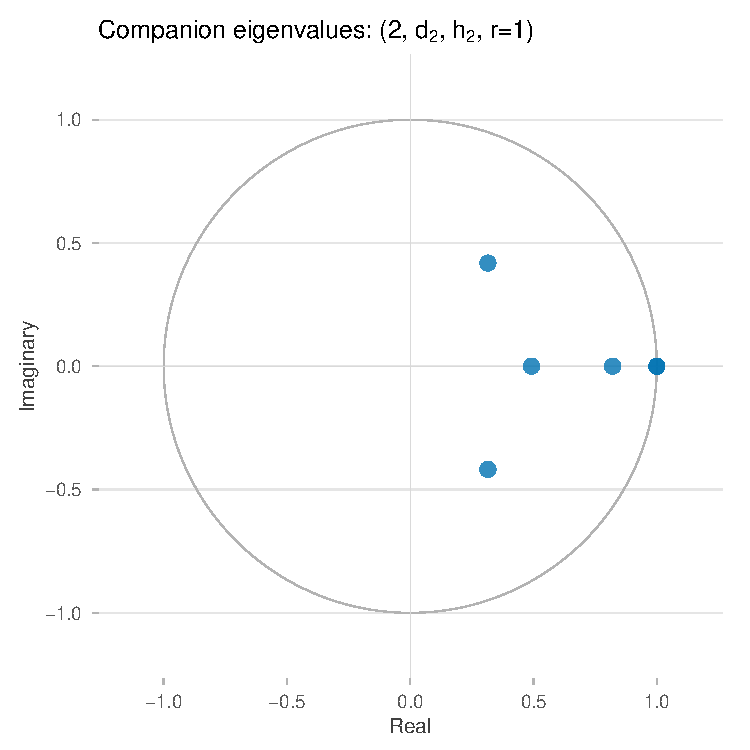
\includegraphics[width=0.7\textwidth]{figures/fig_S2_focal_companion.pdf}
	\caption{Companion matrix eigenvalues, focal specification
		$(p{=}2,\, d_2,\, h_2,\, r{=}1)$}
	\label{fig:S2_companion}
	
	\par\footnotesize\textit{Note:}
	Eigenvalue moduli of the companion matrix. The unit circle is shown
	for reference. Two eigenvalues sit on the unit circle, confirming
	exactly $m - r = 2$ common stochastic trends. All remaining roots
	lie strictly inside, confirming dynamic stability.
	Source: Dataset~1 (1947--2011); script~27.
\end{figure}

\begin{figure}[!ht]
	\centering
	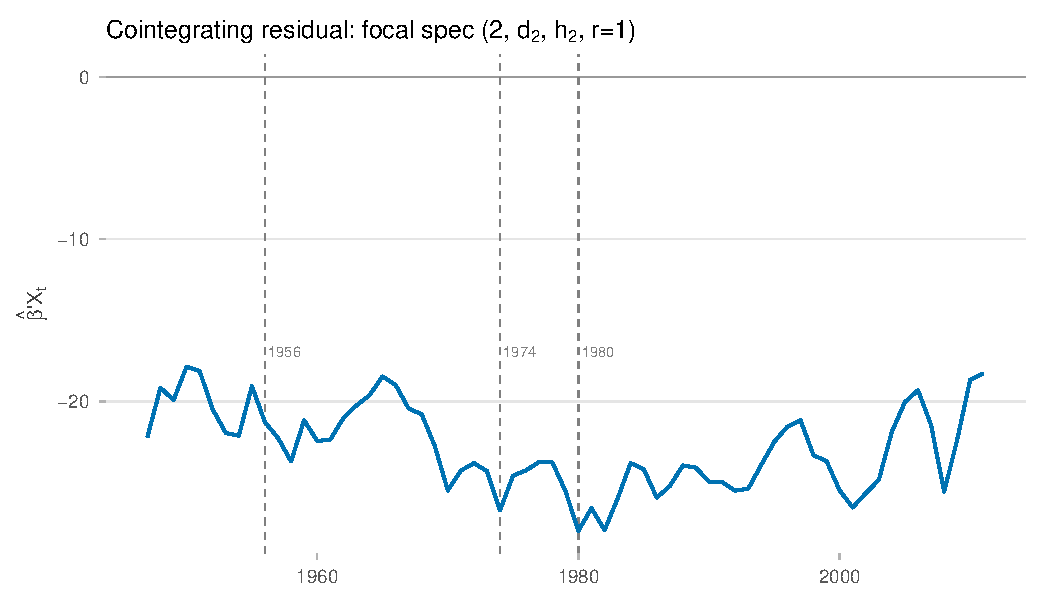
\includegraphics[width=\textwidth]{figures/fig_S2_focal_cu_path.pdf}
	\caption{Cointegrating residual $\hat{\beta}' X_t$, focal specification
		$(p{=}2,\, d_2,\, h_2,\, r{=}1)$}
	\label{fig:S2_focal_residual}
	
	\par\footnotesize\textit{Note:}
	This is the raw cointegrating residual
	$\hat{\beta}' X_t = \ln Y_t - 0.727\,\ln K_t + 20.022\,\ln e_t$,
	not the capacity utilization measure. The residual fluctuates around
	$-22.8$ because the large positive loading on $\ln e_t$ (whose values
	are negative throughout the sample) produces a persistent negative
	level; the mean is absorbed by the $d_2$ deterministic structure.
	The structural objects derived from this residual --- the capacity
	utilization path $\hat{u}_t$ and the reserve-army
	relation~(\ref{eq:S2_reserve_army}) --- are presented in
	Figures~\ref{fig:S2_focal_cu_exploitation}
	and~\ref{fig:S2_focal_scatter}.
	Vertical dashed lines mark the $h_2$ break dates (1956, 1974, 1980).
	Source: Dataset~1 (1947--2011); script~27.
\end{figure}
%</ch1appendix>

\end{document}
